\documentclass[12pt,twoside,openright]{report}

% pacchetti
\usepackage{leo_preamble}

\begin{document}

% frontespizio
\newgeometry{top=1.5in, bottom=1in, left=1in, right=1in} % applica lo stile di geometry
\thispagestyle{empty}
\textwidth=450pt\oddsidemargin=0pt

\begin{titlepage}

\begin{center}
{{\Large{\textsc{Alma Mater Studiorum $\cdot$ Universit\`a di Bologna}}}} 
\rule[0.1cm]{15.8cm}{0.1mm}
\rule[0.5cm]{15.8cm}{0.6mm}
\\\vspace{3mm}

{\small{\bf Dipartimento di Fisica e Astronomia “Augusto Righi”\\
Corso di Laurea in Fisica}}

\end{center}

\vspace{23mm}

\begin{center}
{\LARGE{\bf Studio della produzione di (anti)deuteroni \\con Pythia 8 a $\bf{\sqrt{s} = 13}$ TeV}}\\
\end{center}

\vspace{50mm} \par \noindent

\begin{minipage}[t]{0.47\textwidth}

{\large{\bf Relatore: \vspace{2mm}\\
Prof. Andrea Alici\\\\

\bf Correlatore:
\vspace{2mm}\\
Prof. Nicolò Jacazio\\\\}}
\end{minipage}
%
\hfill
%
\begin{minipage}[t]{0.47\textwidth}\raggedleft {
{\large{\bf Presentata da:\\
\vspace{2mm}
Leandro Ye}}}
\end{minipage}

\vspace{40mm}

\begin{center}
%%%%%%%%
Anno Accademico 2023/2024
%%%%%%%%
\end{center}

\end{titlepage}

\restoregeometry % ripristina lo stile di geometry
\newpage \ \thispagestyle{empty} \newpage
\thispagestyle{empty}

\begin{abstract}
La produzione di (anti)deuteroni è di grande interesse nel campo della fisica delle alte energie, perché permette di ottenere informazioni che spaziano da processi QCD come l'adronizzazione dei quark, ai modelli cosmologici sull'origine dell'universo e allo studio della materia oscura.

In questa tesi si è utilizzato PYTHIA come simulatore Monte Carlo (versione 8.312), attraverso il quale si è studiata la formazione di (anti)deuteroni in collisioni pp ad energie del centro di massa $\sqrt s = 13$ TeV.
In particolare è stato effettuato uno studio sui vari canali di produzione del (anti)deuterone e sull'ottimizzazione di alcuni parametri interni di PYTHIA, come il fattore di normalizzazione, mettendo in confronto i dati raccolti dall'esperimento ALICE con quelli generati da PYTHIA.

I risultati hanno mostrato una riproduzione qualitativamente fedele dei dati di ALICE; tuttavia sono ancora presenti dei disaccordi che suggeriscono la necessità di ulteriori miglioramenti del modello. 
\end{abstract}

\newpage \ \thispagestyle{empty} \newpage

\setcounter{page}{5}
\tableofcontents

\chapter*{Introduzione}
\markboth{Introduzione}{Introduzione}
\addcontentsline{toc}{chapter}{Introduzione}
Recenti misurazioni sperimentali hanno dimostrato come i meccanismi di produzione di (anti)nuclei leggeri non siano stati ancora completamente compresi.
In questo contesto i deuteroni, ossia i nuclei degli atomi di deuterio ($^2_1$H$_1$), essendo i nuclei più leggeri e quindi più abbondantemente prodotti, rivestono un’importanza fondamentale.
Tra gli esperimenti in funzione a LHC, ALICE è quello maggiormente adatto a tali misurazioni grazie alla sua eccellente capacità di identificazione delle particelle cariche su un ampio intervallo di impulsi.
Lo scopo principale dell'esperimento ALICE riguarda lo studio della materia nucleare in condizioni estreme di temperatura e densità di energia, e delle proprietà dello stato della materia chiamato \emph{plasma di quark e gluoni} (Quark-Gluon Plasma, QGP) caratterizzato da quark e gluoni deconfinati.
Si ritiene che negli istanti iniziali successivi al Big Bang la materia di cui era composto l’universo primordiale si sia trovata in questa fase particolare, per cui attraverso lo studio delle sue proprietà è possibile ricavare informazioni essenziali sulla formazione e sull'evoluzione dell'universo.
Lo studio dei processi di nucleosintesi effettuati in ALICE ha quindi un ruolo importante nella ricerca sulle origini dell'universo.

Un altro motivo per lo studio della produzione dei deuteroni è la ricerca della materia oscura: gli antinuclei potrebbero infatti provenire da decadimenti di ipotetiche particelle di materia oscura, ossia delle \emph{Weakly Interactive Massive Particle} (WIMP).
Di conseguenza è possibile usare la produzione di antinuclei come verifica dei modelli di WIMP, perché l'antimateria è una presenza rara nell'universo odierno in confronto con la materia ordinaria. 
Di conseguenza indagare sulla formazione di nuclei leggeri è imperativo in questo contesto.

Lo studio della produzione di deuteroni offre un importante banco di prova per la verifica dei modelli teorici proposti; ad oggi i modelli che rappresentano lo stato dell'arte per la produzione deuteronica sono: 
\begin{itemize}
    \item \emph{modello di coalescenza}, nel quale si assume in sostanza la formazione del deuterone nel momento in cui un protone e un neutrone sono sufficientemente vicini nello spazio delle fasi.
    Notare come questo modello consideri solo un canale di produzione del deuterone, ossia $p+n\to D$, e il suo corrispettivo canale dell'antideuterone rispettivamente.
    Di seguito indicheremo con $D$ e $\bar D$ i deuteroni e gli antideuteroni.
    
    \item \emph{modello di adronizzazione statistica} (o modello termico-statistico), il quale si basa sulla produzione di nuclei leggeri a partire da una sorgente in equilibrio termico, attraverso un approccio più statistico anziché dinamico come nel modello di coalescenza.
    In questo caso, il rateo di produzione dei vari nuclei dipende sostanzialmente dalla loro massa, dal raggio e dalla temperatura del sistema. 
\end{itemize}
Mettendo in confronto questi due modelli con i dati di LHC non si osserva ancora, entro le incertezze sperimentali, che un modello sia preferibile rispetto all'altro.
In particolare, il modello di coalescenza descrive meglio i dati a basse molteplicità, mentre il modello termico-statistico risulta più accurato ad alte molteplicità.

% obiettivi e scopi della tesi
In questa tesi invece viene ripreso un altro modello per la produzione deuteronica, ossia il \emph{modello di sezioni d'urto efficaci} (o modello di Dal-Raklev), implementato nel generatore Monte Carlo \ttbox{PYTHIA 8.3}.
Questo modello, descritto in \cite{Dal_2015}, punta a riprodurre i dati sperimentali con un approccio più probabilistico, in termini di sezioni d'urto efficaci appunto, considerando più possibili canali di produzione, a differenza del modello di coalescenza che ne considera solo uno.
Successivamente, comparando i risultati di questo modello con i dati sperimentali, si esegue un'ottimizzazione dei parametri, e viene fatto un confronto con il modello di coalescenza, cercando di mostrare quale predizione sia migliore nella riproduzione dei dati sperimentali di ALICE.
Infine, si è studiato quali siano i canali che contribuiscono maggiormente alla produzione deuteronica nel modello.

% struttura della tesi
La tesi è strutturata in 3 capitoli: nel \autoref{ch:alice} verrà introdotto l'esperimento ALICE; nel \autoref{ch:modelli} verranno esposti i due principali modelli teorici per la produzione deuteronica e verrà spiegato il funzionamento di \ttbox{PYTHIA 8.3} e del modello di sezioni d'urto efficaci; infine, nel \autoref{ch:risultati} verranno mostrati i metodi utilizzati per le simulazioni di questa tesi, i risultati ottenuti e le ottimizzazioni dei parametri utilizzati. 

\chapter{\textit{A Large Ion Collider Experiment}} \label{ch:alice}
In questo capitolo verrà fornita una panoramica dell'esperimento ALICE descrivendo i suoi componenti principali e le loro funzioni.
Successivamente, verrà analizzato il contributo di ALICE nella ricerca nella fisica nucleare delle alte energie, come lo studio del plasma di quark e gluoni. 
Infine, verranno introdotti i tipi di collisioni analizzate da ALICE, concentradosi sulle collisioni ione-ione, evidenziandone il ruolo cruciale per riprodurre in laboratorio le condizioni primordiali dell'universo e per investigare le proprietà fondamentali della materia.

%%%%%%%%%%%%%%%%%%%%%%%%%%%%%%%%%
\section{L'esperimento ALICE}
L'esperimento \emph{A Large Ion Collider Experiment} (ALICE) \cite{The_ALICE_Collaboration_2008} fa parte del complesso del \emph{Large Hadron Collider} (LHC), il più grande e più potente acceleratore di particelle al mondo \cite{Lyndon_Evans_2008}.
L'LHC è situato sul confine franco-svizzero nella regione di Ginevra, e si trova all'interno di un tunnel sotterraneo che raggiunge una profondità fino a 175 m.
Lungo l'anello dell'LHC sono stati realizzati quattro principali esperimenti: ALICE, CMS, LHCb e ATLAS.
Essi sono disposti secondo lo schema riportato in \autoref{fig:LHC}.
\begin{figure}[htb]
    \centering
    \includesvg[width=0.7\textwidth]{image/1-alice/LHC.svg}
    \caption{Rappresentazione schematica delle posizioni dei quattro grandi esperimenti di LHC, indicati dai punti gialli. "p" e "Pb" indicano gli acceleratori lineari dei protoni e degli ioni di Pb, PS è il \emph{Proton Synchrotron}, SPS il \emph{Super Proton Synchrotron}. (Autore: \href{https://it.m.wikipedia.org/wiki/File:LHC.svg}{Arpad Horvath}).}
    \label{fig:LHC}
\end{figure}
Il centro di ricerca responsabile dell'LHC è l'\emph{Organizzazione Europea per la Ricerca Nucleare} (CERN), fondato nel 1954 a Ginevra, in Svizzera, e fin da allora si è occupato della ricerca nel campo della fisica nucleare e subnucleare.
L'LHC non è solamente il più grande apparato sperimentale al mondo per dimensione, ma anche per numero di fisici e altri studiosi coinvolti, provenienti da qualunque angolo del mondo, rendendo il CERN senza dubbio una delle collaborazioni scientifiche più importanti del mondo.   
Tuttavia è da menzionare che l'LHC non è sempre in operatività, ma lo è solamente in alcuni periodi chiamati \emph{Run}, i quali durano anni, alternati a periodi di manutenzione e aggiornamento, chiamati \emph{Long Shutdowns} (LS).
Di \textit{Run} ad oggi ce ne sono stati tre (Run 1 2009-2013, Run 2 2015-2018, Run 3 2022-2025) e futuri \textit{Run} sono già stati programmati.
In questa tesi si considereranno i dati raccolti durante il \textit{Run} 2 di LHC.
L'LHC è capace di accelerare protoni e anche ioni pesanti (per esempio Pb) a energie ultra-relativistiche.
Questa versatilità permette lo studio delle particelle e delle loro interazioni ad energie estreme.

L'esperimento ALICE si occupa proprio dello studio della materia adronica nella fase detta Plasma di Quark e Gluoni (QGP), uno stato della materia nel quale i quark e i gluoni sono in uno stato non confinato, ottenuto con valori estremi di pressione e temperatura.
Il QGP è ritenuto essere stato la fase in cui si trovava la materia negli istanti iniziali dell'universo, prima che si formasse la materia adronica ordinaria.
Il QGP risulta essere un sistema composto da particelle che interagiscono per interazione forte, descritta dalla teoria della \emph{Quantum Chromodynamics} (QCD) del modello standard.
Perciò studiare le proprietà di questa fase rende l'esperimento ALICE insieme agli altri grandi esperimenti ad LHC, fondamentale per lo studio dei processi QCD.

In LHC, le particelle cariche vengono accelerate tramite cavità di radio-frequenza (cavità RF) che sono situate lungo la circonferenza dell'LHC e devono operare con una frequenza ben precisa in modo che le particelle possano essere accelerate correttamente.
Le particelle vengono prima accelerate da ferme al di fuori dell'LHC, formando un fascio continuo di particelle.
Successivamente, arrivati a una particolare energia (per un fascio di protoni $\sim 50$ MeV) le particelle vengono separate in pacchetti, e dopo ulteriori accelerazioni vengono immesse nell'LHC.
%%%%
%%%%%%%%%%%%%%%%%%%%%%%%%%%%%%%%%%%%%%%%%%%%%%%%%%
\section{Il rilevatore ALICE e i suoi componenti}
A seguire verrà fatta un'introduzione sulle caratteristiche di un rilevatore in generale e quali sono le grandezze principali, e in seguito sulle principali caratteristiche e componenti del rivelatore ALICE.

\subsection{Caratterizzazione di un rilevatore e le grandezze principali}
Lo scopo di un rilevatore è quello di determinare le caratteristiche della particella, come la sua identità (i.e. la sua massa), l'impulso, il suo vertice di origine, l'energia e altre caratteristiche.
Per semplificare il processo di misura si definiscono delle grandezze associabili alle particelle.
Consideriamo un generico rilevatore di forma cilindrica con al suo centro il punto di interazione (IP) e con l'asse rivolto lungo l'asse $z$.
Considerando ora una particella che viene emessa dall'IP (magari dopo uno scattering) con quadrimpulso iniziale (in \textit{}{natural units}) $p^\nu = (E,\vec p)$, con $\vec p = (p_{x}, p_{y}, p_{z})$.
Questa prosegue il suo cammino finché non interagisce con il rilevatore.
L'\emph{impulso trasverso} $p_t$ della particella è definito come 
\begin{equation}
    p_t^2 = p_x^2 + p_y^2
\end{equation}
e la sua \emph{rapidità} come 
\begin{equation}
    y = \dfrac12 \ln\left(\dfrac{E+p_z}{E-p_z}\right)
\end{equation}
Le utilità di queste grandezze è che il primo è invariante per boost lungo l'asse $z$, visto che coinvolge solamente le componenti trasversali, mentre la seconda è una misura di quanto una particella sia direzionata verso l'asse $z$.
Infatti se la particella viene emessa in una direzione giacente nel piano $xy$, si ha che $p_z=0$ perciò $y=0$.
Se invece la direzione è coincidente con l'asse $z$ si ha che $E = \pm p_z$ (supponendo un regime ultra-relativistico per cui $|\vec p| \gg m$) e quindi $y\to \pm\infty$.
Applicando un boost lungo l'asse $z$ la rapidità si trasforma seguendo la seguente espressione ($y\to y'$)
\begin{equation}
    y' = y + \dfrac12\sqrt{\dfrac{1-\beta}{1+\beta}}
\end{equation}
quindi la rapidità varia di una costante legata al boost effettuato.
Un altro vantaggio nell'utilizzare questo parametro è che la differenza di rapidità tra due particelle nel loro sistema di riferimento è uguale a quella nel sistema di riferimento del laboratorio, ossia che $y_1-y_2 = y_1'-y_2'$.

Tuttavia negli esperimenti non sempre viene utilizzato questo parametro, perché richiede la conoscenza sia di $E$ che di $p_z$.
Quindi si procede a definire la \emph{pseudorapidità}, definita come 
\begin{equation}
    \eta = -\ln\tan\dfrac\theta2
\end{equation}
con $\theta$ l'angolo di scattering, ossia l'angolo tra l'asse del cilindro e la direzione di $\vec p$.
Negli esperimenti di LHC viene usata questa variabile al posto della rapidità perché con $p\gg m$ (e quindi $E\approx p$) si ha che $y\approx \eta$, il che ne spiega l'utilizzo.
In \autoref{fig:cms} si mostra una rappresentazione schematica del sistema di coordinate utilizzato convenzionalmente nei rilevatori di LHC.

\begin{figure}[htb]
    \centering
    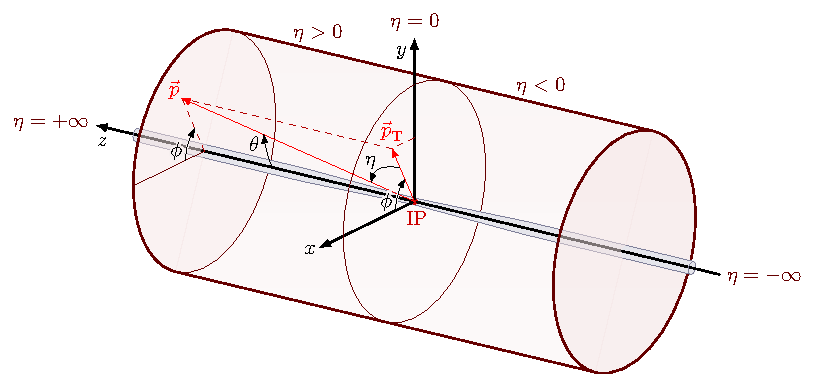
\includegraphics[width=0.9\textwidth]{image/1-alice/axis3D_CMS.pdf}
    \caption{Rappresentazione schematica del sistema di coordinate di un rilevatore in generale di LHC. "IP" è il punto di interazione, $\phi$ è l'angolo assiale, $\theta$ è l'angolo di scattering, $\eta$ è la pseudorapidità. Le particelle provengono da $-\infty$ dell'asse $z$. (Autore: \href{https://tikz.net/axis3d_cms/}{Izaak Neutelings})}
    \label{fig:cms}
\end{figure}

\subsection{Caratteristiche e principali componenti di ALICE}
Il rilevatore ALICE, ossia il complesso dei rilevatori dell'esperimento ALICE, è situato nel Punto di Interazione 2 (IP2) di LHC.
Esso è costituito da una massa di 10,000 tonnellate, lungo 26 m, alto e largo 16 m.
Occupandosi di ioni pesanti, esso deve assicurarsi di gestire bene le problematicità legate alle alte densità di particelle cariche (al tempo di design erano previste 8000 particelle cariche per unità di pseudo-rapidità, a rapidità centrali $|\eta|<1$).
Per questo motivo, per assicurarsi di ottenere delle misure di alta qualità, è necessario l'utilizzo di sensori con elevata granularità e risoluzione spaziale. 
Inoltre esso deve garantire di poter di misurare particelle che, avendo massa maggiore, verranno prodotte con l'impulso trasverso $p_t$ minore, e allo stesso modo poter effettuare la misura di particelle con $p_t$ maggiore.
Quindi, affinché ALICE possa misurare queste particelle, è necessario che il rivelatore possa ricostruire particelle in un intervallo di $p_t$ ampio, nello specifico da 100 MeV/$c$ a 100 GeV/$c$.

La struttura di ALICE è molto complessa, ma si possono individuare due parti principali:
\begin{itemize}
    \item una sezione centrale ("\emph{central barrel}") dove sono collocati i rilevatori più importanti, la maggior parte disposti geometricamente in una configurazione a guscio cilindrico.
    Questi sensori sono racchiusi da un magnete solenoidale (\emph{L3 Magnet}) che genera un campo magnetico uniforme, in direzione del suo asse, con un'intensità di $0.5$ T, necessario per la misura dell'impulso per le particelle cariche.
    In questa sezione si svolgono le mansioni più importanti di ALICE, ossia l'IDentificazione delle Particelle (PID), il tracciamento della traiettoria e la determinazione di processi che avvengono a una pseudo-rapidità di $|\eta| < 1$;
    \item una sezione esterna al magnete solenoidale per la rilevazione di muoni e comunque per misure a una pseudo-rapidità di $-4<\eta<-2.5$.
    In questa zona è presente anche un altro magnete detto \emph{magnete dipolare} con il compito di filtrare particelle indesiderate e permettere la misura dell'impulso dei muoni.
\end{itemize}
Una raffigurazione con le principali componenti di ALICE è riportata in \autoref{fig:alice}.

\begin{figure}[htb]
    \centering
    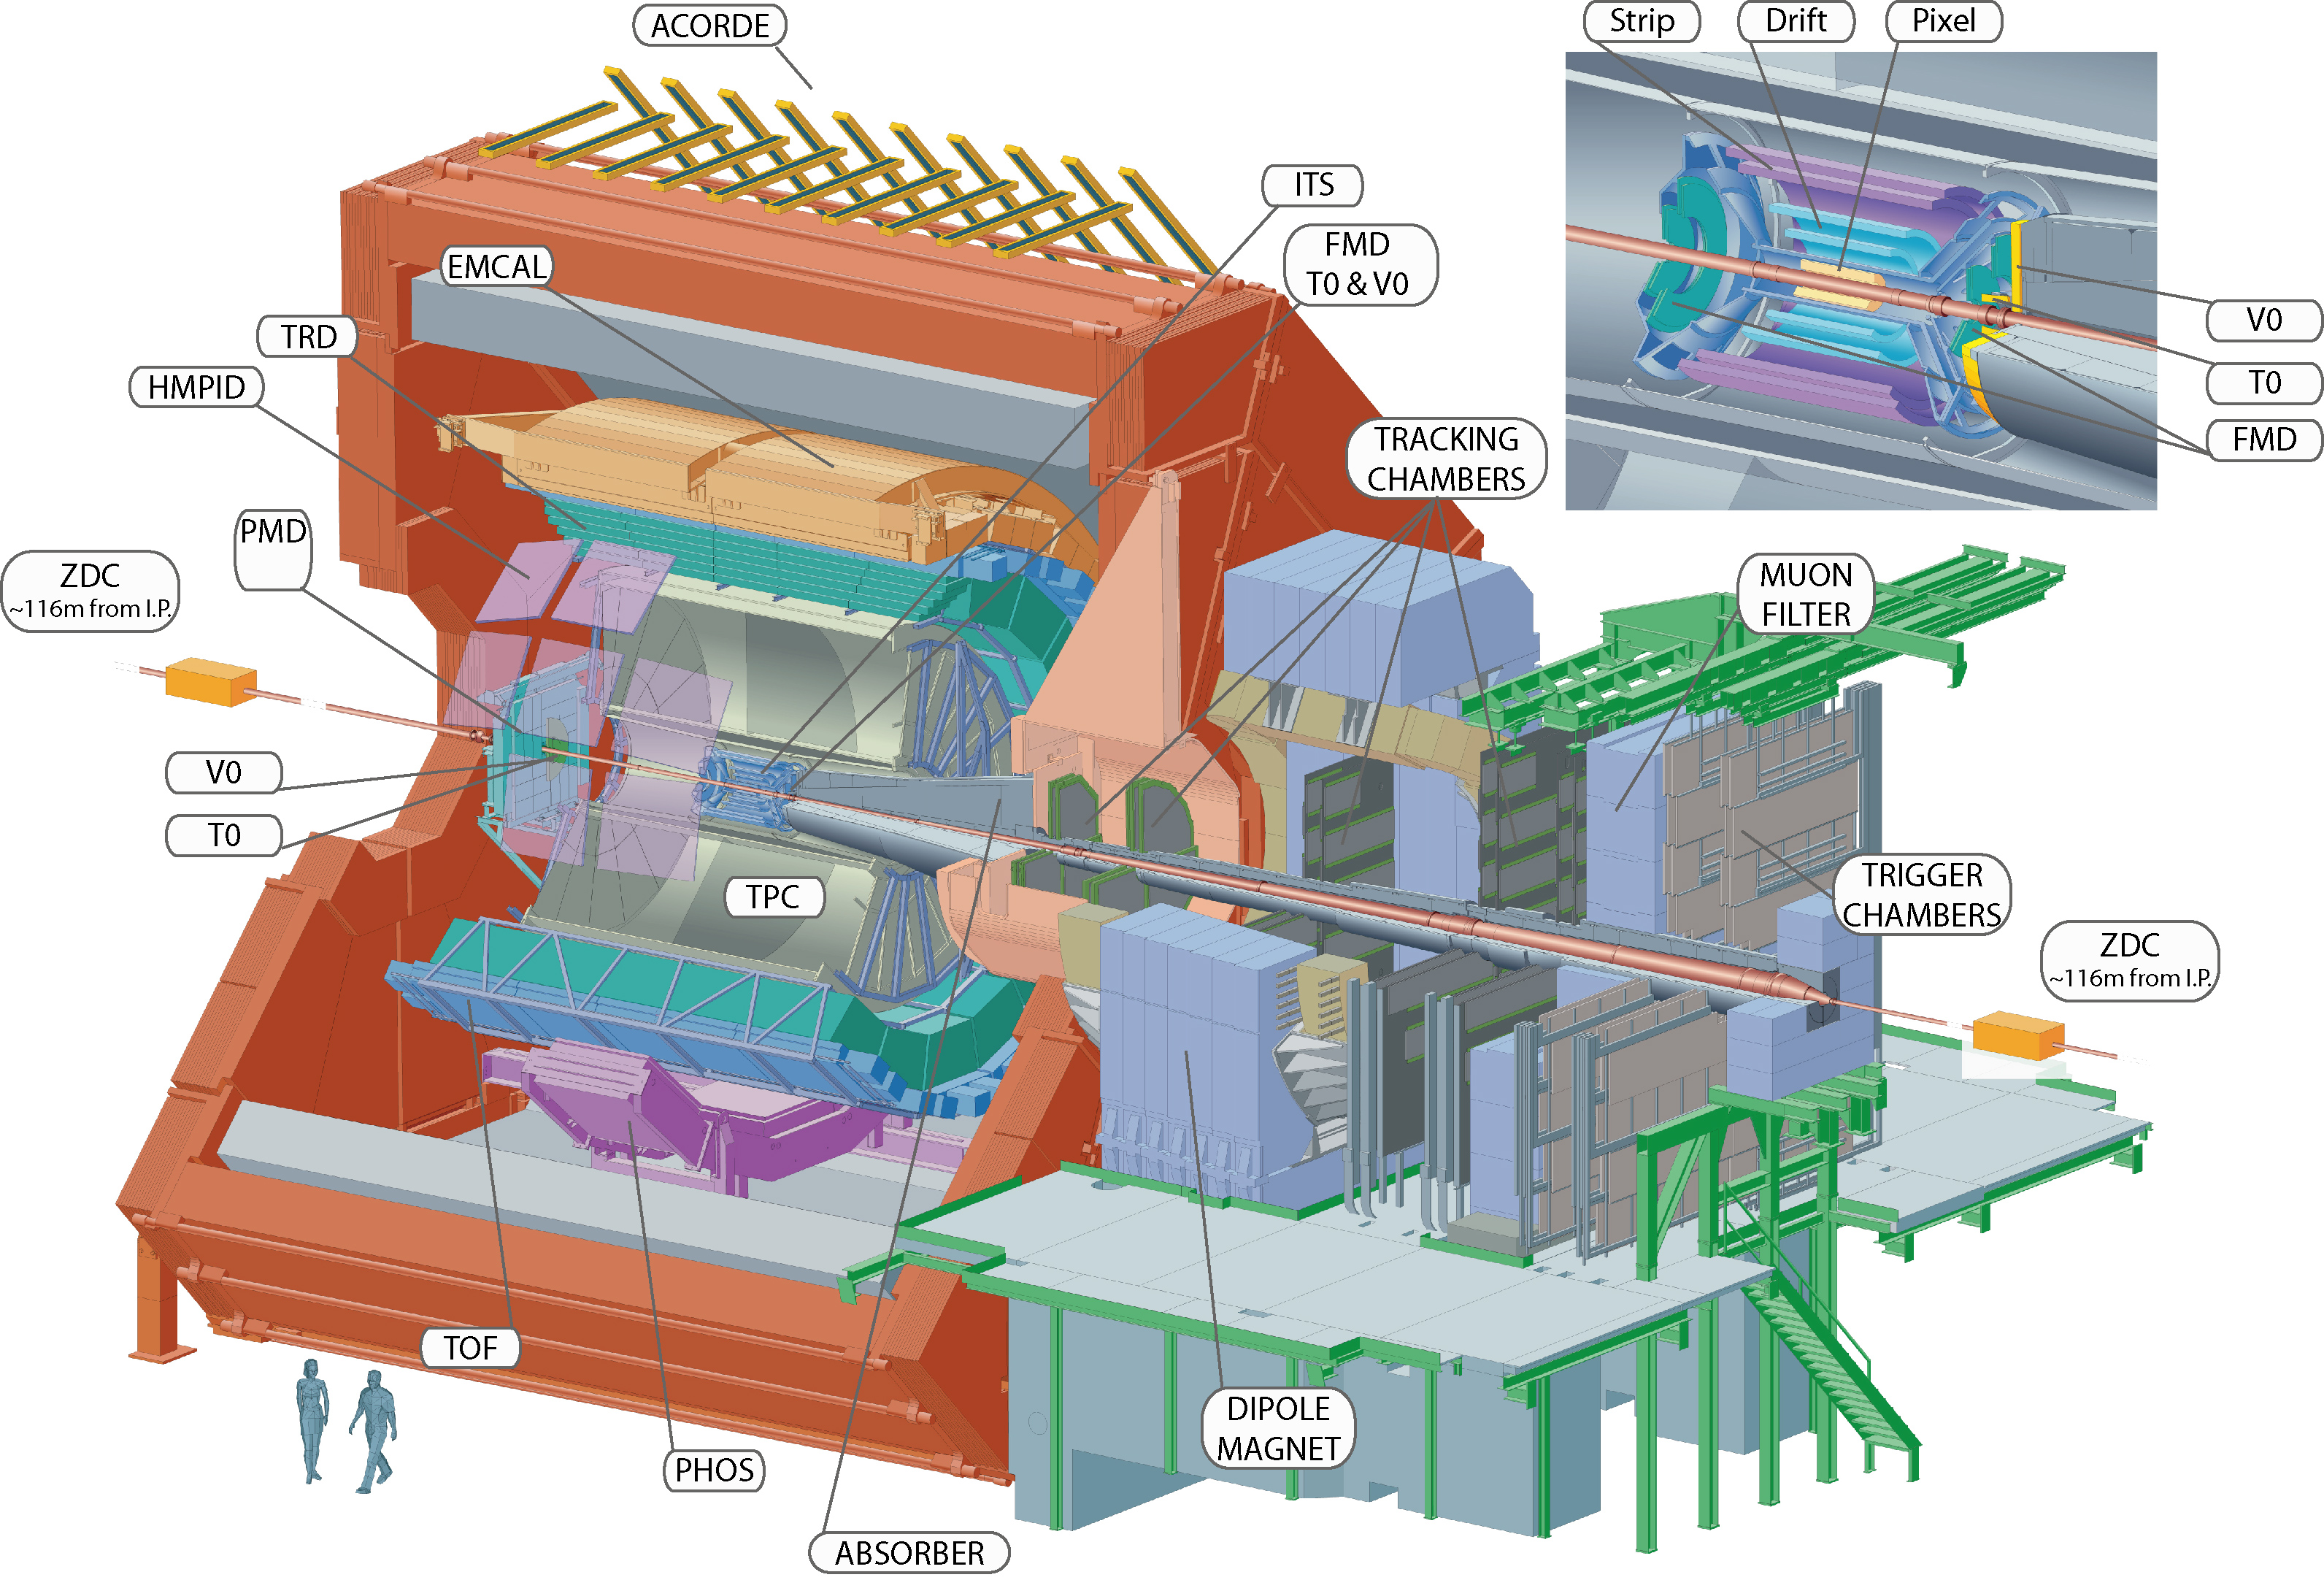
\includegraphics[width=\textwidth]{image/1-alice/alice.jpg}
    \captionwithsource{Schematica dei principali rilevatori presenti in ALICE. La struttura rossa che incapsula il \textit{central barrel} è l'\emph{L3 Magnet}.}{\href{https://en.wikipedia.org/wiki/ALICE_experiment\#/media/File:2012-Aug-02-ALICE_3D_v0_with_Text_(1)_2.jpg}{Wikimedia Commons}.}
    \label{fig:alice}
\end{figure}
Come già anticipato, nel \textit{central barrel} vi sono i rilevatori più importanti per la misura degli osservabili fisici.
Si elencano tramite una lista questi rilevatori, a partire da quello più interno a quello più esterno.

\subsubsection{L'\textit{Inner Tracking System} (ITS)}
L'\emph{Inner Tracking System}, con un diametro di appena 87 cm, ha il compito di localizzare i vertici primari delle collisioni, di ricostruire i vertici secondari, di identificazione di particelle con basso impulso trasverso ($p_t \sim 100$ MeV/$c$), tutto attraverso l'utilizzo di rilevatori al silicio, disposti in 6 piani concentrici.
L'ITS, essendo il rilevatore più interno, deve assicurarsi di raccogliere i dati con più precisione possibile perché è più vicino al luogo di interazione tra le particelle, quindi raccoglierebbe le particelle con minor vita media.
Per esempio i due stati più interni possiedono un potere risolutivo migliore di 100 \si{\micro\metre}.

\subsubsection{La \textit{Time Projection Chamber} (TPC)}
La \emph{Time Projection Chamber} è il principale rivelatore di tracciamento del \textit{central barrel}.
Essa presenta una simmetria assiale, con al centro un elettrodo ad alto voltaggio, e la superficie esterna che fa da gabbia di Faraday.
Con questa struttura le dimensioni del raggio interno ed esterno assumono il valore di $\sim 85$ cm e di $\sim 250$ cm rispettivamente.
Il compito principale della TPC è quello di misurare l'impulso di particelle cariche e di effettuare PID misurando l'energia persa per unità di distanza $dE/dx$, per particelle con $|\eta| < 0.9$.
Per la misura di questa grandezza, il volume interno è riempito con un gas (che durante \textit{Run} 2 consisteva in una miscela composta all'88\% da Ar e al 12\% da CO$_2$).
La particella perde energia per ionizzazione rilasciando  elettroni che quindi migreranno verso gli elettrodi, e il numero di elettroni rilevati sarà proporzionale alla perdita di energia della particella nel gas.

\subsubsection{Il rilevatore \textit{Time Of Flight} (TOF)}
Il rilevatore di tempo di volo \emph{Time-Of-Flight} consiste in una griglia cilindrica di rilevatori a piani resistivi multi-gap (MRPC), i quali misurano il tempo di volo delle particelle ottenendo in questo modo la loro velocità tramite la quale, insieme alla quantità di moto, è possibile ottenere la massa.
Il rilevatore ha una superficie di 141 \si{m^2} e riesce a misurare particelle con pseudo-rapidità centrale ($|\eta| < 0.9$).

\subsubsection{Il rilevatore \textit{High Momentum Particle IDentification} (HMPID)}
Il rilevatore di HMPID è dedicato all'identificazione di adroni carichi con $p_t > 1$ GeV/$c$, quindi serve come ausilio alla PID per gli altri rilevatori elencati in precedenza.
Tuttavia, questo strumento non riesce a rilevare particelle con $|\eta| >0.6$, limitando la statistica disponibile.

\subsubsection{Altri rilevatori}
Altri rilevatori sono:
\begin{itemize}
    \item Gli \emph{Zero Degree Calorimeter}, usati ad esempio per contare il numero di nucleoni spettatori, cioè che non partecipano alla collisione;
    \item Il \emph{V0 detector}, composto da due griglie circolari di scintillatori, ognuno posto sull'asse di collisione in punti opposti rispetto al punto di interazione, misurando in questo modo particelle con alta rapidità.
    Essi funzionano emettendo un segnale con intensità proporzionale al numero di particelle che li attraversano, dunque possono essere usati per la determinazione della molteplicità e della centralità a seconda della collisione considerata;
    \item Il \emph{T0 detector}, formato da due contatori Cherenkov, collocati nella stessa modalità in cui sono disposti i \textit{V0 detector}.
    Vista la disposizione spaziale, anch'essi si occupano di particelle con alta rapidità.
    Una delle loro funzioni è quella di fornire una misura precisa del tempo di collisione degli eventi, necessaria per le misure del tempo di volo.
    Esse possono essere anche utilizzate per la determinazione della posizione del vertice, tuttavia con minore precisione ($\pm 1.5$ cm).
\end{itemize}

L'identificazione di nuclei e antinuclei leggeri in ALICE viene effettuata attraverso la misura della perdita di energia specifica ($dE/dx$) e del tempo di volo delle tracce cariche effettuata da TPC e TOF, rispettivamente.
Ogni particella, infatti, assume un proprio andamento caratteristico della perdita di energia $dE/dx$ in funzione della quantità di moto.
A dimostrazione, la \autoref{fig:pid} mostra alcuni rari candidati di $^4\overline{\text{He}}$ identificati con successo nella presa dati del 2011 \cite{refId0_exotica}.
\begin{figure}[ht]
    \centering
    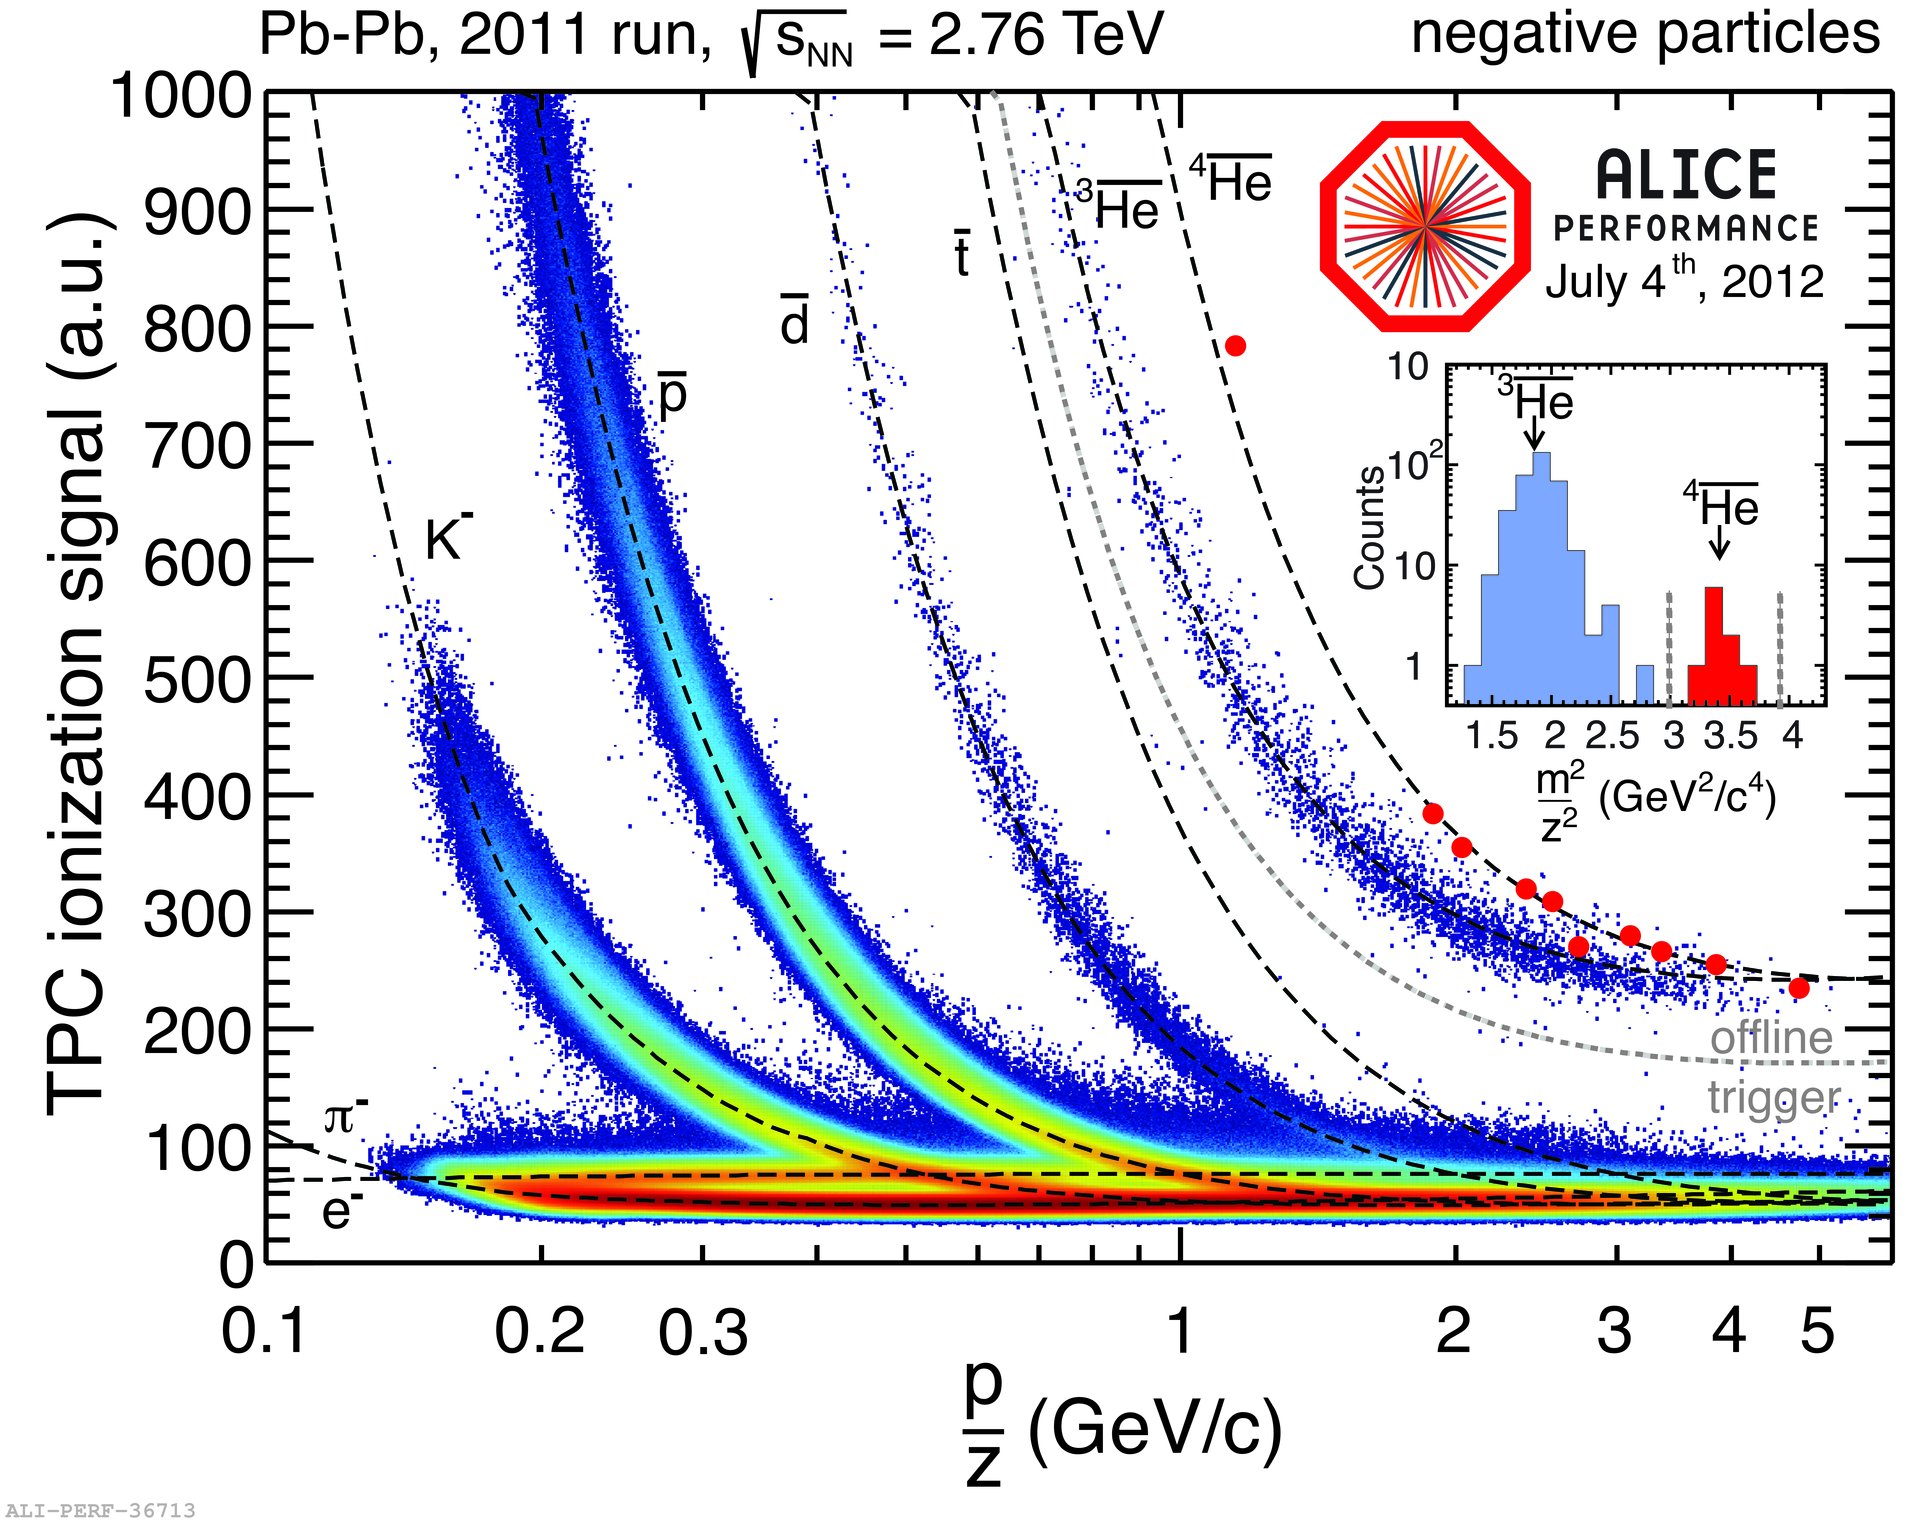
\includegraphics[width=0.7\linewidth]{image/1-alice/PID.png}
    \captionwithsource{Spettro misurato dalla TPC della perdita di energia specifica di particelle con carica negativa. Le linee tratteggiate rappresentano le previsioni teoriche, mentre i punti rossi rappresentano i candidati di $^4\overline{\text{He}}$ selezionati utilizzando la misura del tempo di volo delle anti-particelle. $\bar d$ rappresenta gli antideuteroni, $\bar t$ indica gli anti-trizi.}{\cite{refId0_exotica}}
    \label{fig:pid}
\end{figure}
%%%%%%%%%%%%%%%%%%%%%%%%%%%%%%%%%%
\section{Il ruolo dell'esperimento ALICE}\label{ch:objectives_alice}
Come già anticipato, ALICE lavora su molti punti della ricerca nel campo della fisica delle particelle.
Coinvolgendo collisioni tra particelle pesanti, ALICE gioca un ruolo fondamentale nel rispondere al quesito dell'origine dell'universo.

\subsection{Studio della formazione nucleare}
Il principale obiettivo di ALICE è quello di studiare lo stato del plasma di quark e gluoni, il quale è ritenuto essere stato lo stato della materia negli istanti iniziali dell'universo, e in particolare la transizione da questa fase alla materia ordinaria, processo chiamato adronizzazione.
Infatti ALICE, tramite LHC e le collisioni di ioni pesanti, riesce a riprodurre e analizzare questo stato della materia, caratterizzato da temperature e pressioni estreme.
Tuttavia è importante menzionare che questo stato della materia ha vita breve, dell'ordine di $\sim10^{-23}$ s (come vedremo successivamente), e si misurano solamente i prodotti di decadimento, che consistono di particelle ordinarie come protoni, neutroni e nuclei leggeri, con le corrispettive antiparticelle.
Quindi ALICE si occupa anche dei meccanismi di formazione di nuclei che non sono ancora del tutto compresi; studiare la produzione dei (anti)nuclei leggeri potrebbe fornire informazioni su questi meccanismi e permettere di testare i modelli teorici che sono stati sviluppati per descriverli.

Più dettagli saranno forniti nel prossimo capitolo.

\subsection{Materia oscura}
Si studiano gli (anti)nuclei anche per un altro scopo, ossia la ricerca di materia oscura.
Si considera la materia oscura come la componente attrattiva dominante della gravità, ma, non potendola osservare direttamente, possiamo conoscere solamente alcune proprietà di essa, attraverso misure delle velocità di rotazione delle galassie, dispersione di velocità delle galassie ellittiche, lenti gravitazionali o comunque tramite osservazioni astronomiche.
Una eventuale scoperta della materia oscura porterebbe senz'altro a una rivoluzione senza precedenti nella fisica moderna.

Ad oggi abbiamo diversi modelli per caratterizzare la natura della materia oscura, in seguito ne elenchiamo alcuni: l'ipotesi barionica della materia oscura, per cui si ipotizza la composizione barionica della materia oscura; i modelli non barionici, come il modello degli assioni, ipotetiche particelle molto leggere e caratterizzate da elevate velocità, oppure il modello dei neutrini; infine, il più promettente, il modello dei WIMP.
Quest'ultimo modello, introdotto da Steigman e Turner \cite{STEIGMAN1985375_wimp}, ipotizza l'esistenza delle particelle massive debolmente interagenti, in acronimo WIMP (\emph{Weakly Interacting Massive Particle}). 
L'abbondanza di materia oscura può essere spiegata da questo modello, in particolare dal meccanismo di \emph{freeze-out} termico, nella quale il sistema, passando dal QGP, si espande così velocemente che la velocità dell'espansione dell'universo supera la velocità di interazione delle particelle.
Perciò si possono considerare i WIMP come i relitti termici dell'universo. 
Sebbene non siano stati ancora osservati sperimentalmente, neanche indirettamente, si predice che i WIMP annichilino e decadino in (anti)materia ordinaria (per esempio antiprotoni e antineutroni), i quali possono interagire formando stati legati, ossia antinuclei leggeri.
Questi possono invece costituire un segnale rilevabile, con energia cinetica di 0.1-1 GeV alla produzione, senza problemi di eventuali fondi cosmici, dal momento in cui alcuni dei modelli di WIMP predicono un flusso massiccio di antinuclei leggeri con ordini di grandezza in più rispetto a quello del fondo, come per esempio si può vedere in \autoref{fig:he3} per il nucleo di $^3\overline{\text{He}}$.
\begin{figure}[htb]
    \centering
    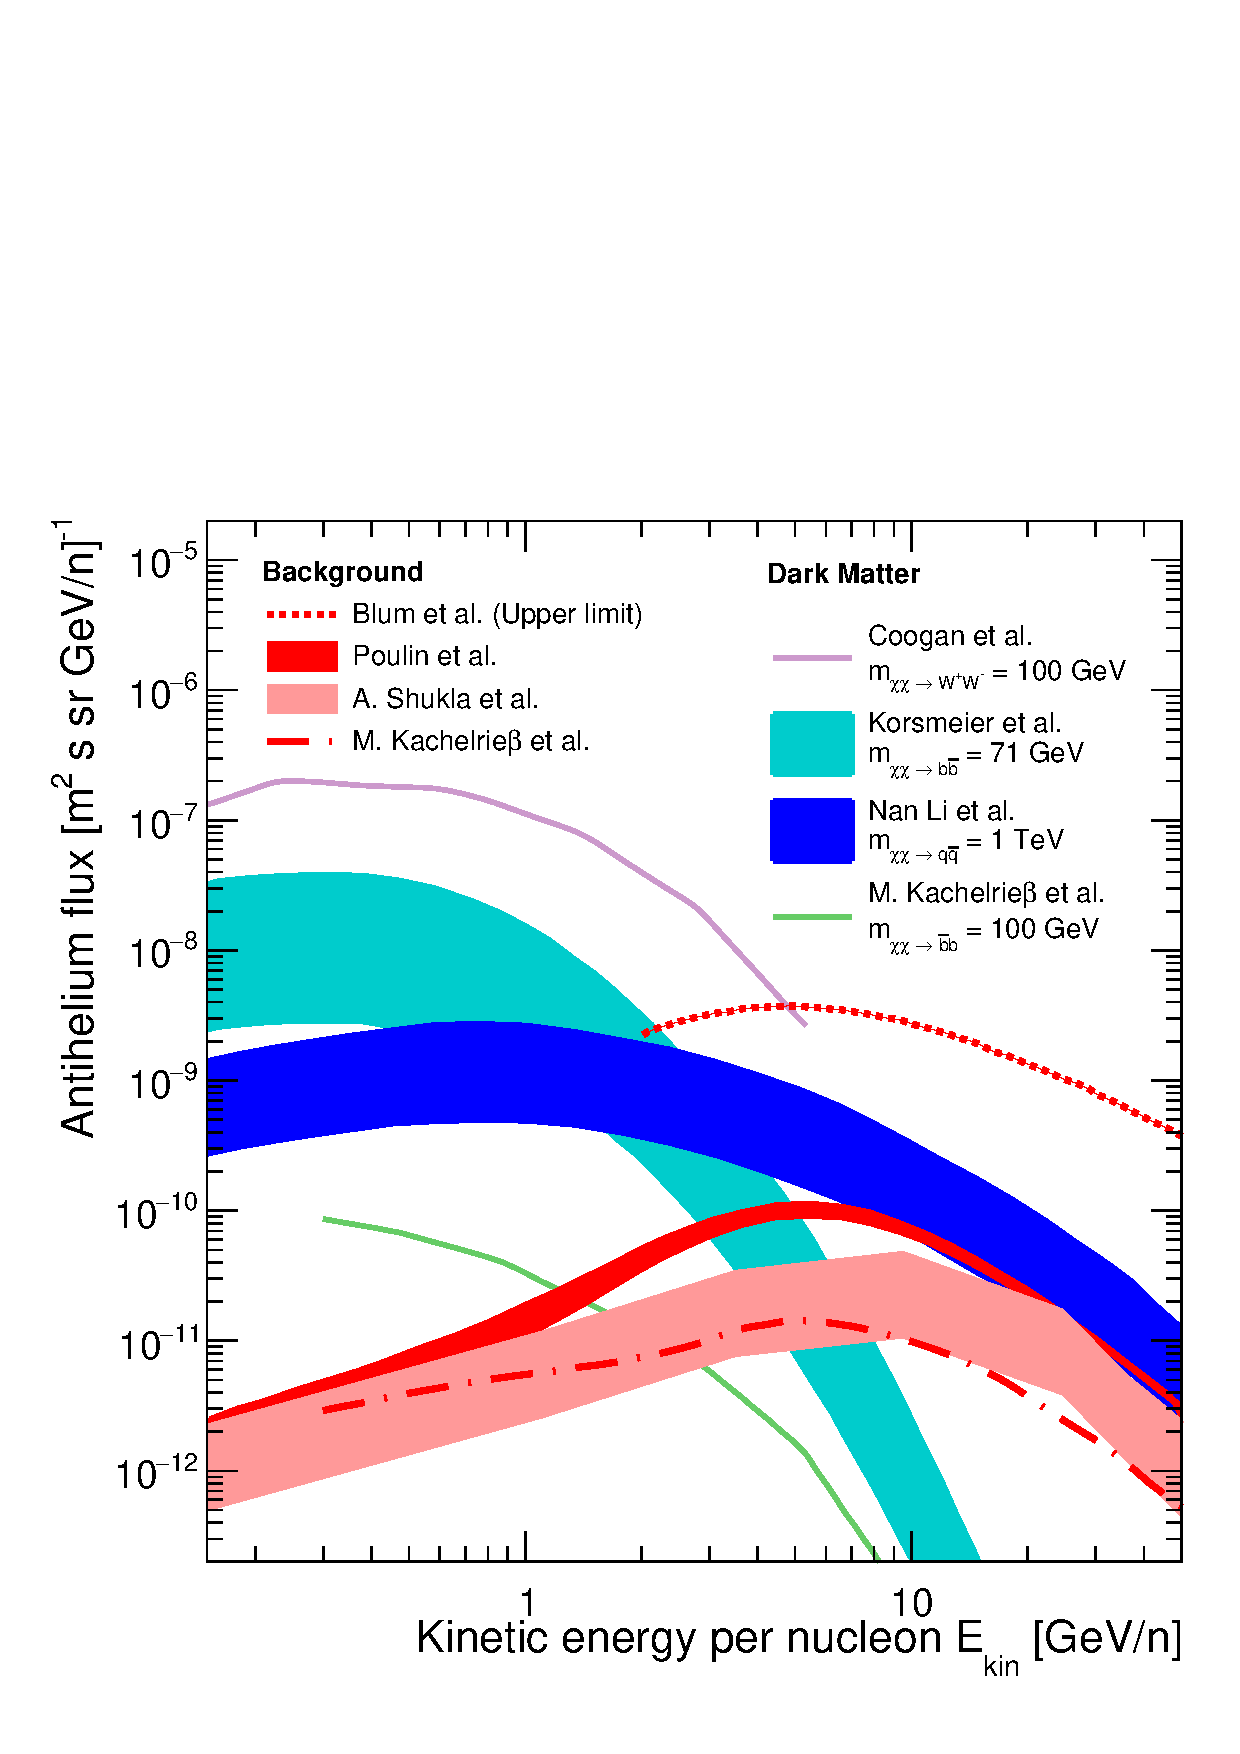
\includegraphics[width=0.6\textwidth]{image/1-alice/He3.pdf}
    \captionwithsource{Il flusso di $^3\overline{\text{He}}$ (in azzurro) in funzione dell'energia cinetica secondo più modelli di WIMP provenienti dalla letteratura scientifica, in confronto con il fondo cosmico (in rosso).}{\cite{Doetinchem_2020}.}
    \label{fig:he3}
\end{figure}

\subsection{La ricerca dei nuclei}
Per riuscire a studiare le proprietà degli (anti)nuclei è necessario come prima cosa riuscire a misurarli.
Tuttavia si noti che il numero di nuclei che viene prodotto in collisioni adroniche è molto ridotto, per cui un esperimento effettuato con un valore insufficiente dell'energia del centro di massa $\sqrt s$ comporta una percentuale molto bassa di (anti)nuclei prodotti.

Per quantificare questo numero, si considera che la formazione di un antinucleone è corrisposta necessariamente alla formazione di un nucleone, per conservazione del numero barionico.
Tenendo in considerazione ciò allora l'energia $\sqrt s$ dovrebbe assumere un valore molto più alto inizialmente.
% Per esempio per aggiungere il deuterone nel sistema è necessario l'aggiunta di 17 GeV in $\sqrt s$ \cite{2011STAREeuteronEormationEnergy}.
In generale nella letteratura si assume che venga prodotto un nucleo in ogni circa 1000 nucleoni prodotti, per nucleone del nucleo. 
Inoltre è necessario ricordare che in un evento di collisione il numero barionico deve essere conservato, per cui se l'energia iniziale è sufficientemente bassa, si vedrà uno sbilanciamento in numero, in particolare si avrà che il numero di antinuclei che vengono prodotti è più basso rispetto al numero di nuclei.
Per esempio, esperimenti condotti all'acceleratore \emph{Intersecting Storage Rings} (ISR) del CERN negli anni Settanta con collisioni pp ad energie del centro di massa di $\sqrt s \sim 50$ GeV hanno misurato un rapporto $D/\bar D$ di circa $4$ \cite{Gibson_Duane_Newman_Ogren_Henning_Jarlskog_Little_Sanford_Wu_B&Oslash;ggild_etal._2008}.

Per ovviare a questo problema è sufficiente aumentare il valore di $\sqrt s$.
Al LHC, l'energia è sufficientemente alta per poter portare il valore del rapporto di nucleo$/$antinucleo vicino a 1.
Per vedere questo, indicando con $D$ e $\bar D$ i deuteroni e gli antideuteroni rispettivamente, in \autoref{fig:ratio_of_matter/antimatter} riportiamo il grafico della frazione di $\bar p/p$ e di $\bar D/D$, dove si può osservare un avvicinamento al valore unitario con l'aumentare dell'energia.
\begin{figure}[htb]
    \centering
    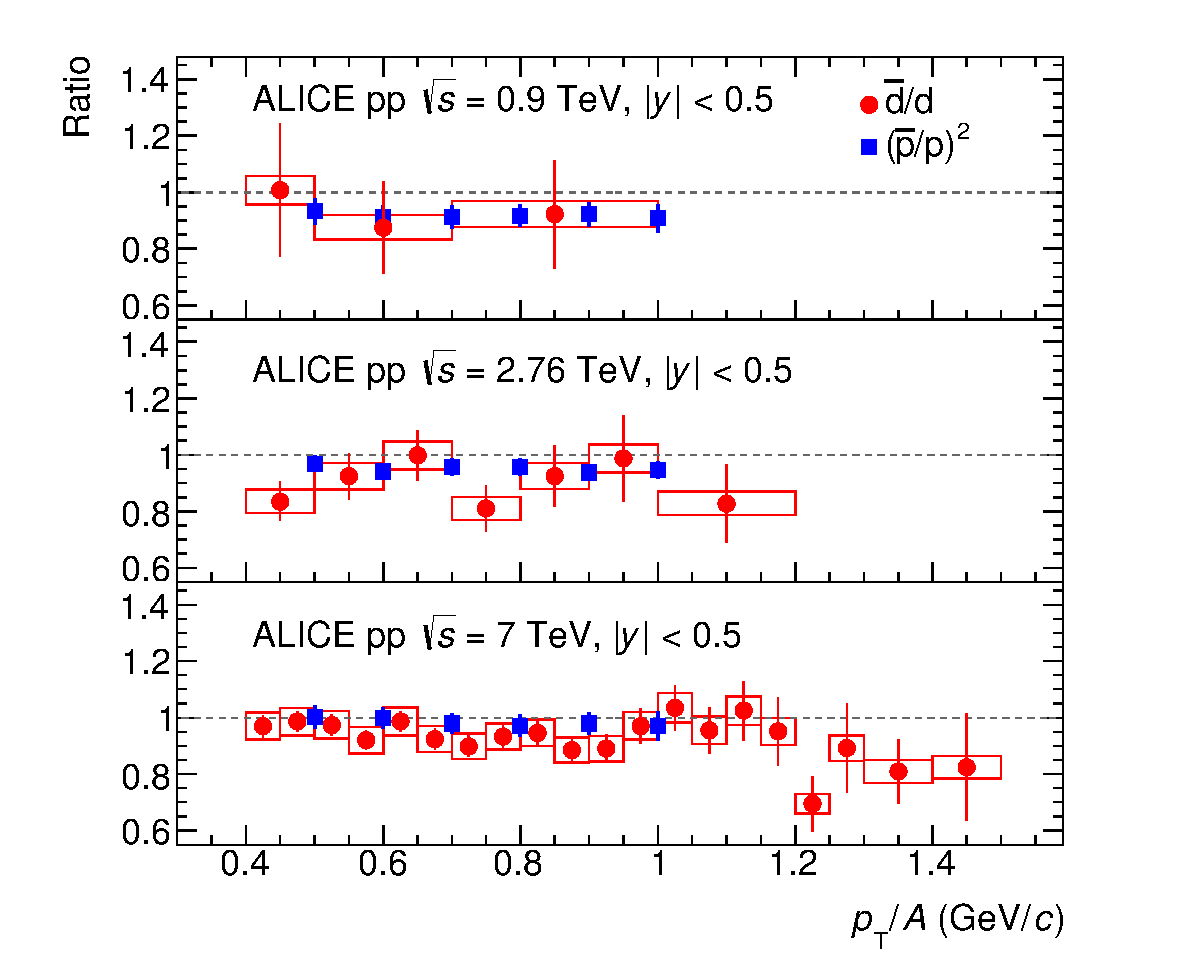
\includegraphics[width=0.7\textwidth]{image/1-alice/DbarDRatio.pdf}
    \captionwithsource{Andamento del rapporto di $\bar D/D$ (qui indicato con $\bar d/d)$ in funzione di $p_t$ per nucleone sovrapposta al rapporto quadro di $\bar p/p$, ai tre valori di energia indicati.}{\cite{Acharya_2018}.}
    \label{fig:ratio_of_matter/antimatter}
\end{figure}

\section{Collisioni in ALICE}
In questa sezione si cerca di introdurre la fisica delle collisioni riguardanti le collisioni ultrarelativistiche di ioni.

Nel Modello Standard si descrivono tre delle quattro forze fondamentali: la forza forte, la forza elettromagnetica, la forza debole in ordine di intensità.
Dalla teoria della cromodinamica quantistica (QCD) si sa che ogni nucleone è composto da quark, i quali interagiscono tramite l'interazione forte attraverso lo scambio di gluoni.
Dalla QCD inoltre sappiamo che il gluone in realtà non è altro che un quanto di energia dei campi mediatori della forza forte, e tramite un'invarianza di gauge locale SU(3) si ricavano 8 tipi di gluoni, tutti con carica di colore diversa in modo da formare una base per coprire tutti i colori possibili.\\

\subsection{Il sistema pre-collisione}
Per ricreare le condizioni richieste per la formazione di QGP è possibile far collidere ioni pesanti a regime ultra-relativistico.
In questo regime, con la contrazione di Lorentz lungo la direzione del fascio, gli ioni appaiono come dei dischi piatti (\autoref{fig:pb}), e per questo motivo le dimensioni trasversali del nucleo appaiono più larghe delle dimensioni longitudinali. 
Perciò una collisione tra ioni può essere considerata come la sovrapposizione di collisioni individuali tra i nucleoni provenienti da direzioni opposte.
\begin{figure}[htb]
    \centering
    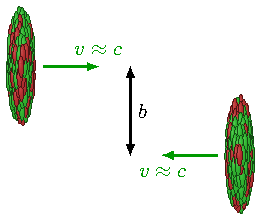
\includegraphics[width=0.5\textwidth]{image/1-alice/PbPb_collisions.pdf}
    \caption{Schema rappresentativo di una collisione Pb-Pb. Le sfere rosse rappresentano i protoni e le sfere verdi i neutroni. (Autore: \href{https://tikz.net/pbpb_collisions/}{Izaak Neutelings})}
    \label{fig:pb}
\end{figure}

È importante notare che non sempre tutti i nucleoni partecipano alla collisione: questo succede se nel piano del fascio i baricentri dei nuclei non non coincidono ma sono separati da una distanza $b$ (parametro di impatto), in questo caso interagiranno soltanto i nucleoni all'interno dell'area di sovrapposizione nucleare. 
I nucleoni non interagenti sono chiamati \emph{spettatori}; i nucleoni che viceversa partecipano alla collisione vengono chiamati \emph{partecipanti}.
Se il numero di nucleoni partecipanti è $N_\text{part}$, il numero di spettatori è $N_\text{spect} = 2A-N_\text{part}$.
Il parametro d'impatto $b$ gioca un ruolo fondamentale nelle collisioni di nuclei: esso determina la centralità di una collisione, una quantificazione della regione di sovrapposizione, e con ciò il numero di nucleoni partecipanti.
%Da questo si può capire che, se si vuole più statistica, è necessario minimizzare questo parametro massimizzando così la centralità della collisione.
Dal momento che la centralità è correlata con la molteplicità di una collisione, ossia il numero di particelle cariche prodotte nella collisione, affinché si possa normalizzare le osservabili tra collisioni differenti, la misura della centralità è fondamentale.

Vi sono due metodi principali per la misura della centralità:
\begin{itemize}
    \item Il primo metodo consiste nella misura diretta della molteplicità, tramite conteggio del numero di particelle cariche prodotte in una collisione.
    Questo metodo è tuttavia dipendente dalla scelta del modello geometrico utilizzato per i processi adronici;
    \item il secondo metodo invece si basa sulla misura dell'energia degli spettatori, in genere effettuata in posizioni di alta molteplicità.
    Questo modello, al contrario del primo, è indipendente dal modello di collisione utilizzato.
\end{itemize}

\subsection{Il sistema post-collisione}
Grazie all'alta densità di energia che si viene a creare nell'urto ultra-relativistico tra ioni pesanti, si viene a formare un sistema che interagisce per l'interazione forte, il QGP.
Lo studio di questo sistema è proprio l'obiettivo di ALICE, ossia quello di andare a indagare lo stato del QGP.
In questo stato l'energia del sistema rende l'interazione forte meno dominante, portando a uno stato deconfinato di materia in cui i quark e i gluoni possono muoversi liberamente.
\begin{figure}[htb]
    \centering
    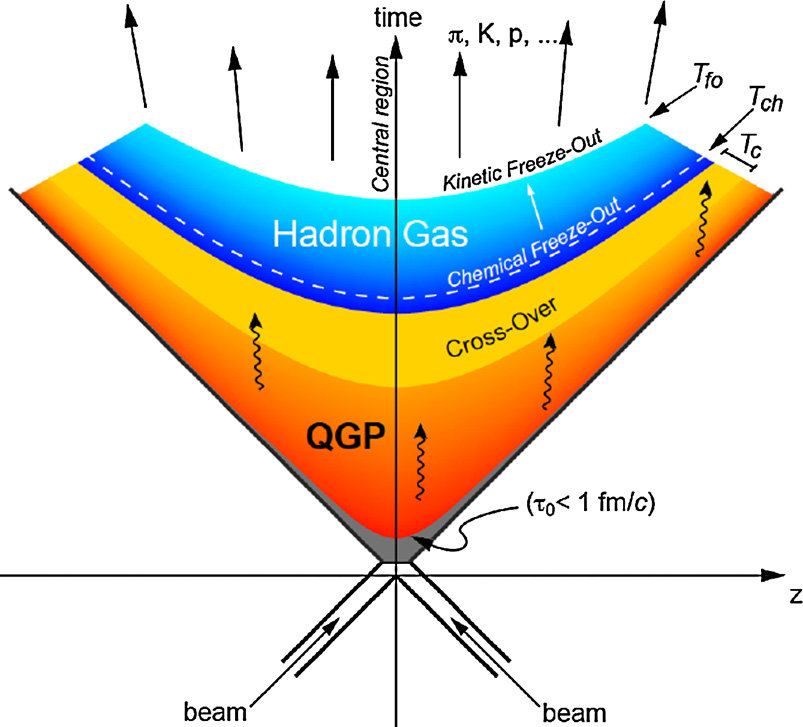
\includegraphics[width=0.7\textwidth]{image/1-alice/Colour-online-Space-time-diagram-of-a-heavy-ion-collision-of-two-nuclei-colliding-at.jpg}
    \captionwithsource{Diagramma spazio-tempo di una collisione di due ioni pesanti ultra-relativistici. La zona grigia sottostante alla QGP rappresenta lo stato di pre-equilibro.}{\cite{QGPbraun}}
    \label{fig:qgp}
\end{figure}

Più precisamente, al momento dell'impatto degli ioni, le singole collisioni coinvolgono scattering "hard" ovvero con un alto trasferimento di impulso che inducono alla produzione di partoni ad alta energia.
In questo momento si distinguono due zone in particolare: la prima a rapidità centrale, dove si è depositata la maggior parte dell'energia, la seconda invece ad alta rapidità, popolata da quark di valenza e particelle spettatori.
Nella zona a rapidità centrale, se la densità di energia è sufficientemente alta, si forma il QGP, sotto forma di \emph{fireball} in equilibrio termico.
In questa fase di equilibrio la \textit{fireball} si espande per via della pressione esercitata alla sua superficie e di conseguenza si ha un calo progressivo della temperatura; una volta che la temperatura sarà scesa al di sotto del valore critico inizia il processo di adronizzazione.
Successivamente, non appena lo scambio di impulso diventa insufficiente per sostenere le interazioni inelastiche, allora si arriva al cosiddetto \emph{freeze-out chimico}, in cui le abbondanze relative delle particelle rimangono invariate.
Nel momento in cui le particelle prodotte non interagiscono più, conservando il loro quadrimpulso, allora si parla di \emph{freeze-out cinetico}.
Infine, dopo $\sim15$ fm/$c = 5\cdot 10^{-23}$ s gli adroni formatisi giungono ai rilevatori.
Uno schema spazio-tempo di quanto appena descritto è rappresentato in \autoref{fig:qgp}.

\chapter{Modelli teorici}\label{ch:modelli}
Nel capitolo precedente si è visto che tra i principali obiettivi fisici dell'esperimento ALICE c'è lo studio del QGP e della transizione da questo stato alla materia ordinaria.
Questa transizione è descritta da diversi modelli teorici in cui la formazione di adroni a partire da quark singoli viene implementata utilizzando processi fisici e formalismi differenti. 
Due modelli largamente utilizzati sono il modello di coalescenza e quello di adronizzazione statistica.

In questo capitolo verranno esposti questi due modelli e verranno effettuati dei confronti tra essi.
Inoltre verrà introdotto il generatore Monte Carlo \pythiaa{} \cite{pythia8300}, nel quale si utilizza un altro modello di formazione basato sul processo di frammentazione di stringa, ossia il modello di sezioni d'urto efficaci. 

\section{Il modello di coalescenza}
Nel modello di coalescenza, i nucleoni generati dalla collisione vanno a formare un nucleo se essi sono vicini nello spazio delle fasi.
Per comprendere meglio, il modello si incentra su un parametro $B_A$, detto \emph{di coalescenza}, il quale è un indicatore della probabilità di formazione del nucleo.
Esso è definito nel seguente modo \cite{alice_2022_coal_formula}:
\begin{equation}\label{eq:coal}
    \dfrac{1}{2\pi p_t^\text{A}}\dfrac{d^2N_\text{A}}{dy\ dp_t^\text{A}} = B_\text{A}({p_t}^\text{p}) \cdot  \left(\dfrac{1}{2\pi p_t^\text{p}}\dfrac{d^2N_\text{p}}{dy\ dp_t^\text{p}}\right)^A
\end{equation}
con p e A che si riferiscono ai (anti)protoni e ai (anti)nuclei con numero di massa $A$, $p_t$ la quantità di moto trasversa del nucleo, $N_p$ e $N_A$ il numero di (anti)protoni e (anti)nuclei rispettivamente.
Il significato dell'\autoref{eq:coal} è il seguente: il membro a sinistra indica gli spettri invarianti di produzione dei (anti)nuclei, mentre il termine a destra è il prodotto tra $B_A$ e gli spettri invarianti di (anti)protoni.\\

Inizialmente il modello di coalescenza si basava su un modello fenomenologico: qualsiasi coppia (anti)protone-(anti)neutrone forma un (anti)deuterone nel momento in cui il modulo della differenza della loro quantità di moto ($|\vec p_p - \vec p_n|$) è minore di un parametro costante $p_0$.
Quindi il processo non è probabilistico, ma deterministico e indipendente dalle dimensioni del sistema considerato e dalla distanza che separa i nucleoni.
Per questo motivo questo modello viene chiamato \emph{modello semplice}.
Questo modello è valido sperimentalmente solamente per le collisioni che prevedono sistemi con dimensioni ridotte, come per esempio le collisioni p-nucleo, mentre per i sistemi più estesi, si osserva sperimentalmente una dipendenza con le dimensioni del nucleo.
Questo modello è utilizzato soprattutto per i simulatori Monte Carlo poiché i meccanismi di formazione sono semplici da gestire.\\

Un modello più adeguato dovrebbe considerare anche le dimensioni del nucleo e che due nucleoni vicini nello spazio dei momenti non necessariamente formano un nucleo, seguendo un approccio stocastico che rispecchi la natura quantomeccanica del processo.
Per avere una descrizione più rigorosa, si utilizzano le funzioni di Wigner per la rappresentazione dello spazio di fase del nucleo \cite{Scheibl_1999_wigner}.
Per esempio nel caso più semplice, quello del deuterone, una possibile funzione d'onda del deuterone può essere scritta sotto forma di una gaussiana, 
\begin{equation}
    \phi_D(\vec r) = (\pi {r_D}^2)^{-3/4}\ \exp\left(\dfrac{-r^2}{2{r_D}^2}\right)
\end{equation}
con $r_D$ il raggio caratteristico del deuterone.

Considerando la natura quantomeccanica delle particelle, è necessario aggiungere un fattore di correzione medio \cite{Scheibl_1999_wigner}.
Questo è definito come
\begin{equation}
    \lrangle{C_A} = \prod_{i=1,2,3}\left(1+\dfrac{r^2}{4R_i^2}\right)^{-\frac{A-1}2}
\end{equation}
con $R_i$ la proiezione del raggio sull'asse $x_i$.
Assumendo un'approssimazione isotropica della sorgente, allora si può dimostrare che il parametro di coalescenza assume la seguente espressione
\begin{equation}
    B_A = \dfrac{2J_A+1}{2^A}\dfrac{1}{\sqrt{A\ m_T^{A-1}}} \left(\dfrac{2\pi}{R^2 + \left(\frac{r_A}{2}\right)^2}\right)^{\frac32(A-1)}
\end{equation}
con $J_A$ e $r_A$ lo spin e il raggio caratteristico del nucleo, $m_t = \sqrt{m^2+p_t^2}$ la massa trasversa e $R$ la dimensione caratteristica della sorgente.
Questa espressione ha senso perché tiene conto sia delle dimensioni della sorgente che di quella del nucleone.
È importante notare che il parametro $B_A$ non dipende solamente dal numero di massa, ma anche dalla specie considerata.
Per esempio se si tiene in conto $^{3}{\rm He}$ e $^{3}{\rm H}$, essi differiscono per il parametro $r_A$, in particolare $r_{^{3}{\rm He}} =  2.48$ fm e $r_{^{3}{\rm H}} = 2.15$ fm \cite{PURCELL20151_nuclear_sheet}.\\

Per mostrare la validità di questo modello si esegue un confronto tra dati di ALICE e le previsioni del modello esposto.
In particolare si confrontano le funzioni dei parametri di coalescenza $B_2$ e $B_3$ in funzione della molteplicità \cite{alice_2022_coal_formula} (\autoref{fig:BAvsMult}).
Per gli andamenti teorici si utilizzano due parametrizzazioni: il primo ("A") è basato sul fit ai dati sperimentali di ALICE del raggio del sistema (effettuato con misurazioni femtoscopiche, \cite{PhysRevD.87.052016_femto}) in funzione della molteplicità; mentre nella seconda ("B") la relazione tra il raggio del sistema e la molteplicità viene fissata per riprodurre il $B_2$ dei deuteroni in collisioni Pb-Pb a una energia nucleone-nucleone $\sqrt{s_{NN}} = 2.76$ TeV.
\begin{figure}[h]
    \centering
    \begin{subfigure}{.49\textwidth}
    \centering
        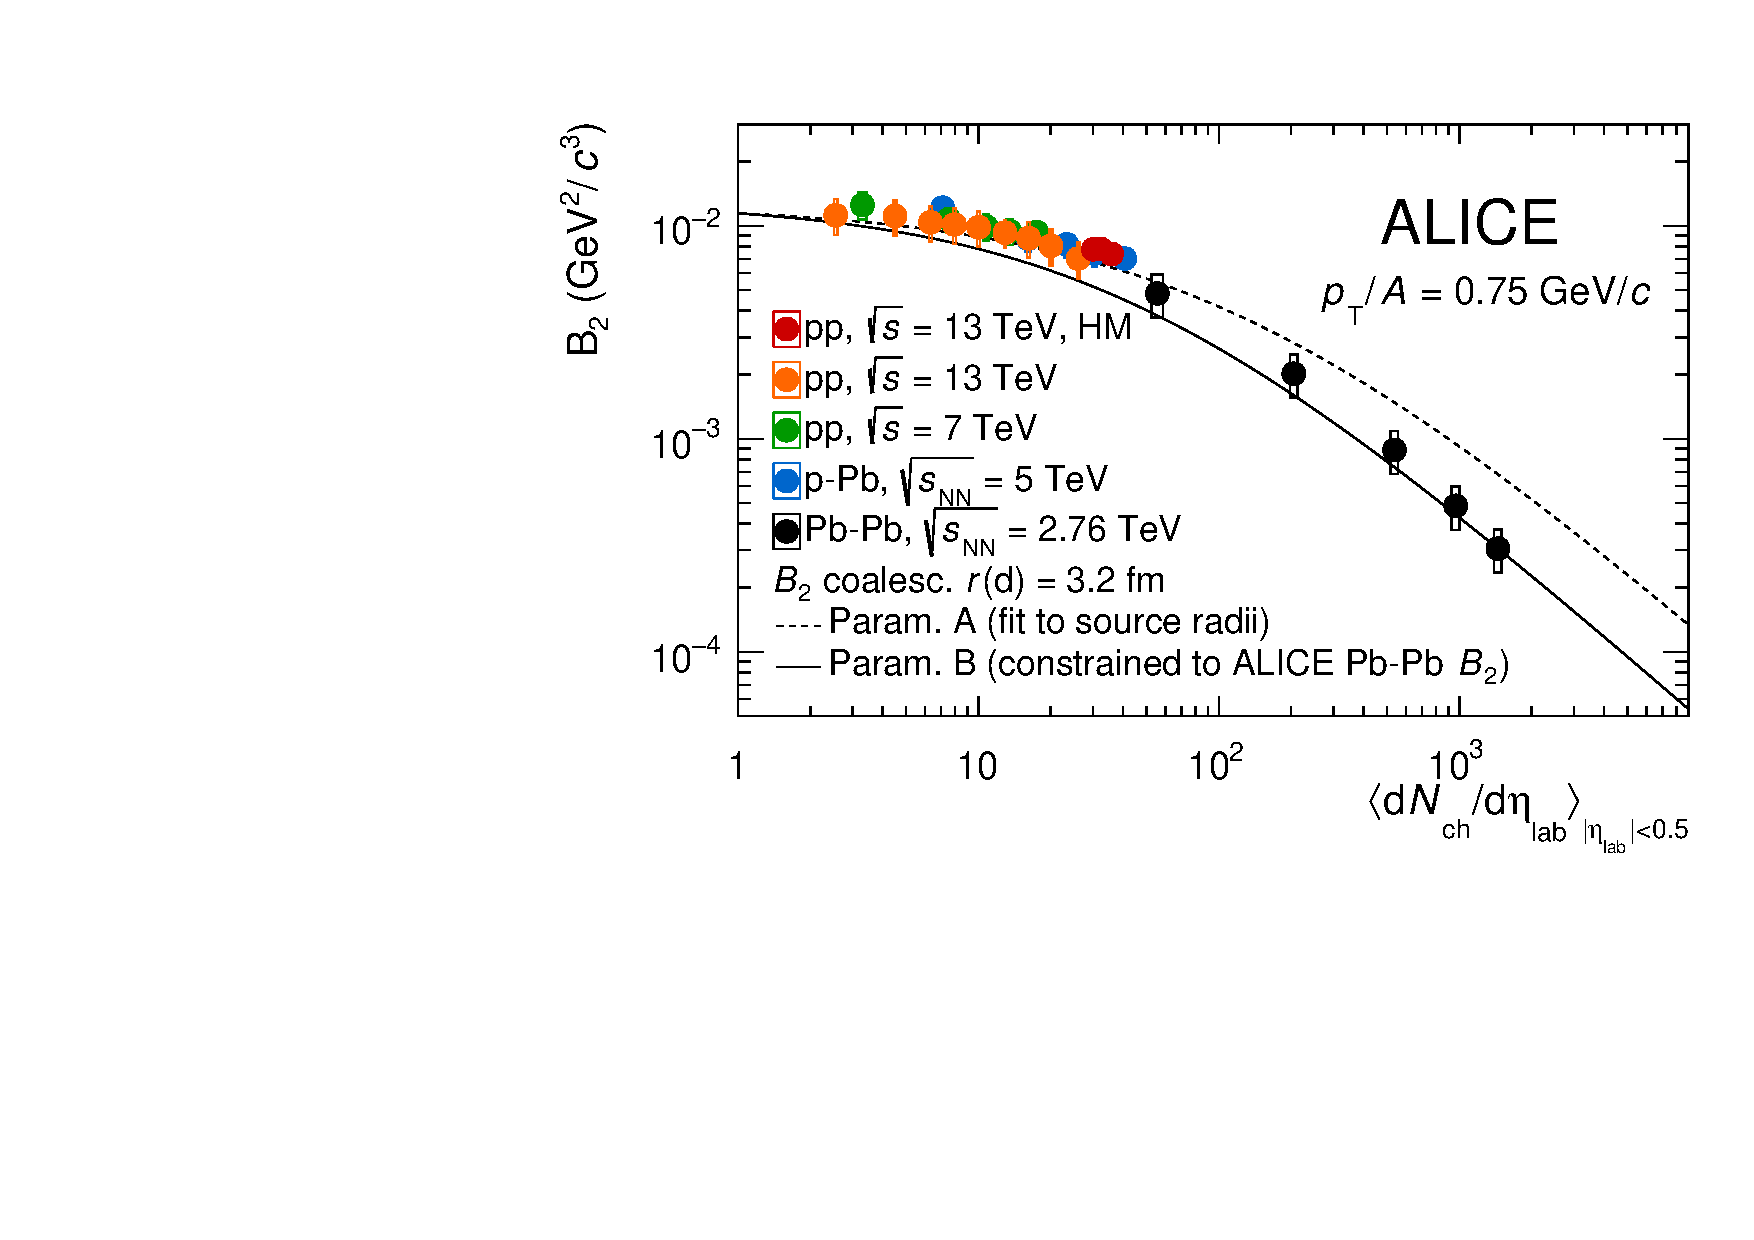
\includegraphics[width=\textwidth]{image/2-modelli/cB2vsMult.pdf}
        \caption{(Anti)deuteroni}
        \label{fig:cB2vsMult}
    \end{subfigure}
    %\hspace{1cm}
    \begin{subfigure}{.49\textwidth}
        \centering
        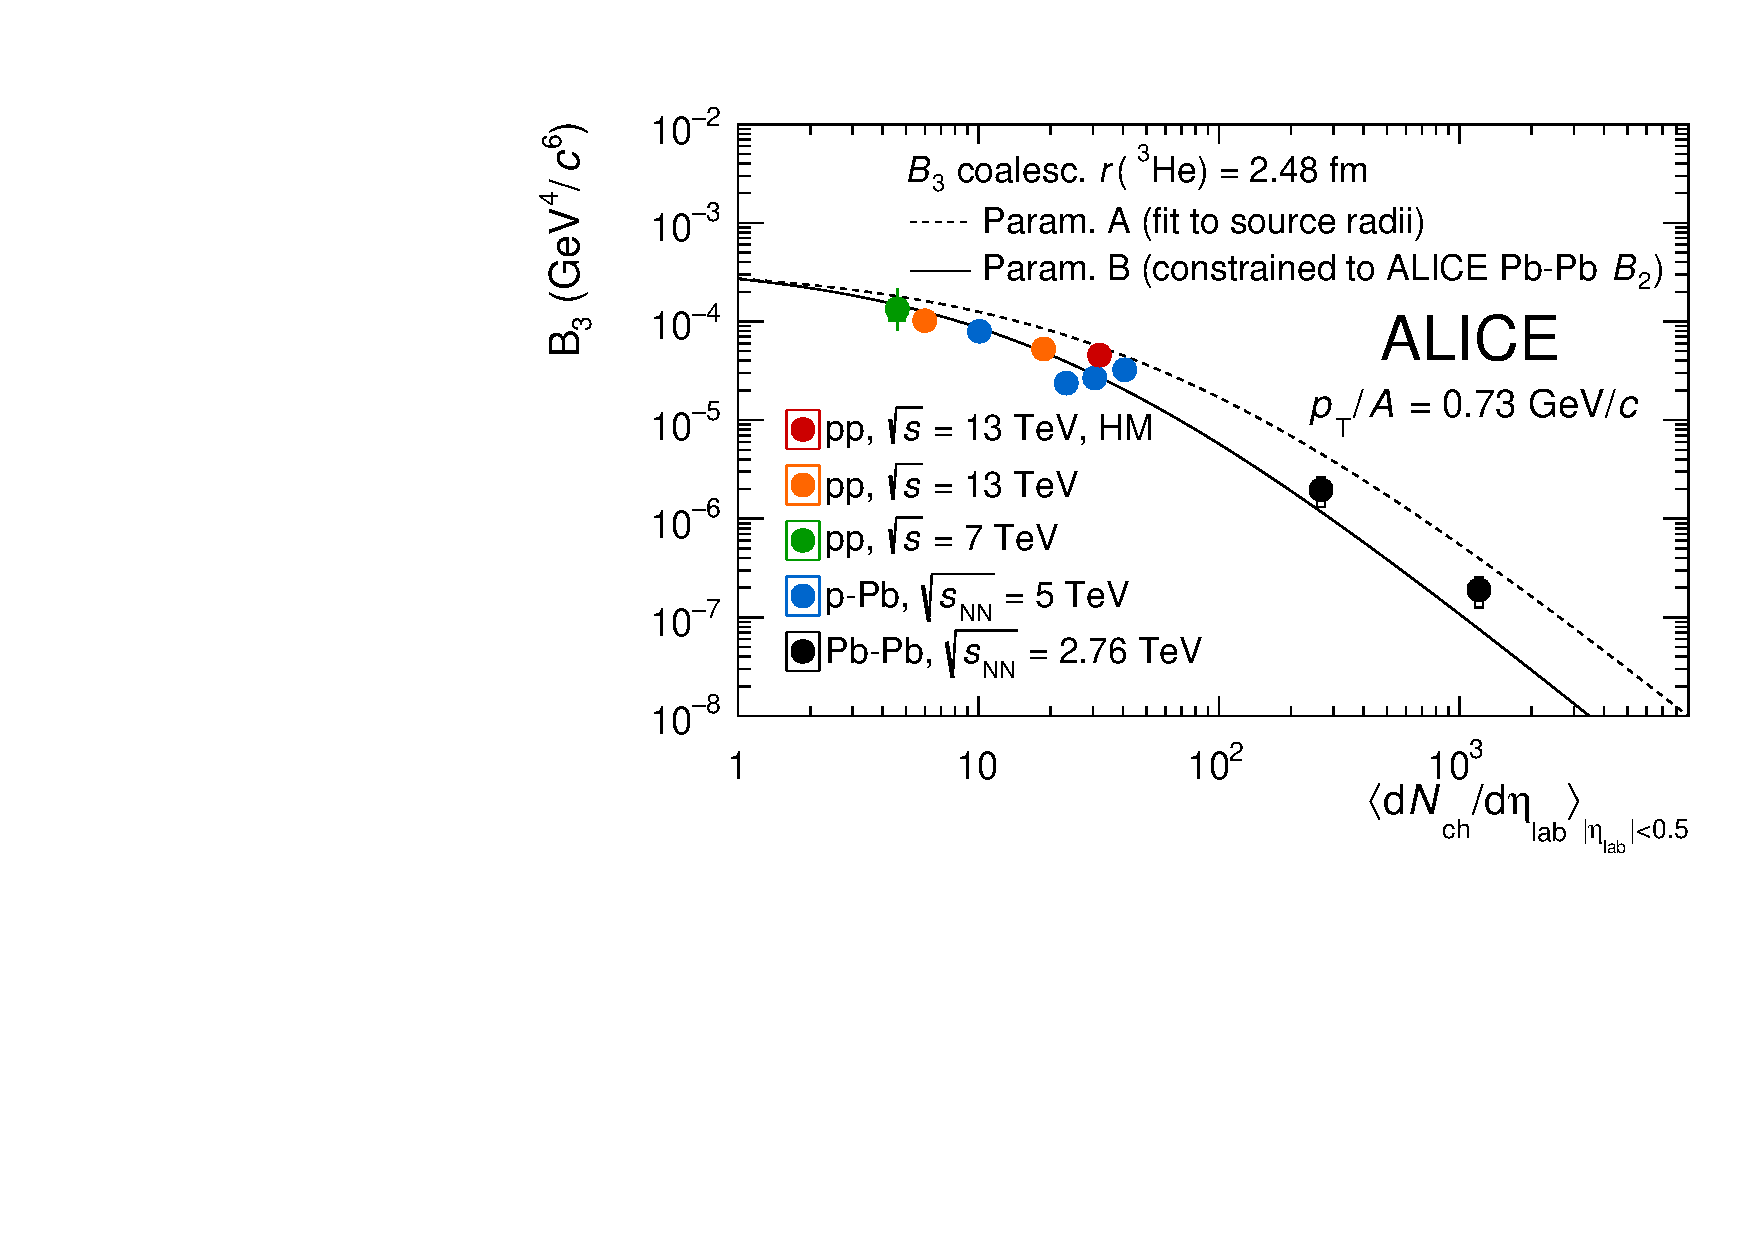
\includegraphics[width=\textwidth]{image/2-modelli/cB3vsMult.pdf}
        \caption{(Anti)elio}
        \label{fig:cB3vsMult}
    \end{subfigure}
    \captionwithsource{Misure (punti colorati) di \emph{\rmfamily (a)} $B_2$ e di \emph{\rmfamily (b)} $B_3$ in funzione della molteplicità effettuate a $p_t/A$ indicate. Le linee rappresentano le previsioni teoriche basate su due diversi parametrizzazioni del raggio della sorgente.}{\cite{alice_2022_coal_formula}} 
    \label{fig:BAvsMult}
\end{figure}
Si osserva che per la misura del parametro $B_2$, nelle collisioni a basse molteplicità (pp e p-Pb) $B_2$ ha una dipendenza debole della molteplicità, mentre per collisioni ad alta molteplicità (Pb-Pb) i dati mostrano un calo sostanziale di $B_2$. 
Analogamente per $B_3$, il modello di coalescenza descrive qualitativamente gli andamenti ma non riesce a farlo per tutto l'intervallo di molteplicità.
%%%%%%%%%%%%%%%%%%%%%%%%%%%%%%%%%%%%%%%
\section{Il modello di adronizzazione statistica}
I \emph{modelli di adronizzazione statistica} (SHM), chiamati anche modelli termici-statistici, sono utilizzati per predire l'abbondanza delle diverse specie di particelle prodotte nelle collisioni di particelle.
Questi modelli assumono che le particelle vengano emesse da una sorgente in equilibrio termico e chimico e che ogni tipo di particella abbia la possibilità di essere prodotta, purché vengano rispettate le leggi di conservazione previste dal Modello Standard.
Le abbondanze relative delle specie che vengono prodotte tuttavia verranno regolate dalle leggi della meccanica statistica, in particolare dipenderanno fortemente dalla funzione di partizione, la quale a sua volta dipenderà dal mezzo in cui avviene la collisione.
Il mezzo che si considera in questo caso è quello di un gas in espansione, non interagente, composto da particelle e risonanze, che chiamiamo \emph{Gas di Risonanze Adroniche} (HRG).
A seconda del sistema  considerato abbiamo due casi principali: se il volume di interazione è sufficientemente grande (per esempio nelle collisioni di ioni pesanti) si utilizza allora il modello statistico con un ensemble gran canonico; mentre se il volume è ridotto allora si utilizza il modello statistico nell'ensemble canonico.\\

Nel formalismo dell'ensemble gran canonico si prevede un sistema che interagisce con un reservoir, scambiando con esso energia e particelle.
Il sistema che si considera in questo caso è la regione misurabile dai rilevatori di ALICE, in contatto con il reservoir che si forma quando vi è una collisione di ioni pesanti, ossia l'HRG (non il Quark-Gluon Plasma perché esso non è invece accessibile dai rilevatori).
Assumendo che vi sia un equilibrio tra la regione e il reservoir, allora ciò implica una conservazione in media dell'energia e delle principali grandezze quantistiche, come la carica e i numeri quantici.
Quindi si utilizza il formalismo gran canonico per ottenere le proprietà statistiche di questi sistemi fisici.
Per far ciò si utilizza la funzione di partizione $Z$ e sapendo che dipende da queste proprietà, possiamo assumere che $Z = Z(T,V,\mu)$, con $T$ la temperatura del mezzo, $V$ il volume, $\mu$ il potenziale chimico collettivo definito come $\mu = \sum_iQ_i\mu_i$, con $\mu_i$ i potenziali chimici relativi a ogni carica conservata $Q_i$.
Nel reservoir, le principali grandezze che vengono conservate sono la carica elettrica $Q$, la stranezza $S$ e il numero barionico $B$.
La funzione gran canonica, data la non-interazione tra le particelle, può essere considerata come prodotto delle funzioni di partizione di singolo stato di particella,
\begin{gather}
    Z(T,V,\mu) = \prod_i Z_i(T,V,\mu_i)\\
    \implies \log Z(T,V,\mu)= \sum_i \log Z_i(T,V,\mu_i)
\end{gather}
Si può dimostrare che la funzione che descrive $\log Z_i$ ha la seguente espressione
\begin{equation}
    \log Z_i(T,V,\mu_i) = \dfrac{Vg_i}{2\pi\beta\pi^2}\sum_{k=1}^\infty \dfrac{(\pm 1)^{k+1}}{k^2}\lambda_i^k m_i^2 \ K_2(k\beta m_i) 
\end{equation}
con $g_i$ la molteplicità spin-isospin della particella nello stato $i$, $m_i$ è la sua massa, $K_2$ la funzione modificata di Bessel del secondo tipo; il termine $\pm$ assume valore $+1$ per particelle descritte dalla statistica di Bose-Einstein e $-1$ per le particelle descritte dalla statistica di Fermi-Dirac.
Una quantità interessante da ricavare è il numero medio di particelle di uno stato $i$, ottenibile da
\begin{equation}\label{eq:mean_n}
    \lrangle{N_i}_\text{th}(T,V,\mu) = \dfrac1\beta\pd{}{\mu_i} \log Z_i(T,V,\mu_i)
\end{equation}
Tuttavia questa descrizione è incompleta dal momento in cui non si è tenuto conto di contributi da parte degli stati di risonanza.
Facendo così si ottiene il numero medio totale di particelle dello stato $i$ come
\begin{equation}
    \lrangle{N_i}_\text{tot}(T,V,\mu) = \lrangle{N_i}_\text{th}(T,V,\mu) + \sum_j \Gamma_{j\to i}\lrangle{N_i}_\text{th}(T,V,\mu)
\end{equation}
con $\Gamma_{j\to i}$ il coefficiente del contributo della risonanza $j$ che decade in $i$.
Quindi il numero medio delle particelle dipende principalmente da cinque parametri, ossia la temperatura, il volume e i tre potenziali chimici.\\

Il modello di adronizzazione statistica canonica (CSM) invece riguarda volumi di interazioni minori ottenuti per esempio in collisioni pp.
Essendo il volume di interazione ridotto, allora la conservazione delle cariche non può essere più assunta in media, ma deve essere esatta, ossia senza fluttuazioni.
Questo significa che il numero di particelle cariche è soppresso rispetto a quello del modello gran canonico, per questo viene dato il nome di \emph{soppressione canonica}.
La trattazione del modello canonico è simile a quello gran canonico: si assume il HRG in equilibrio termico come sistema, caratterizzato da un volume e temperatura, con le cariche conservate ($Q$, $B$ e $S$).
Un fattore aggiuntivo da tenere in considerazione rispetto alla trattazione gran canonica in questo caso è il \emph{fattore chimico}, il quale assicura la conservazione della carica locale.
Uno degli effetti della soppressione canonica è la riduzione della produzione delle particelle con stranezza.\\

\subsection{Predizioni del SHM}
Tramite il modello SHM sono possibili diverse predizioni:
\begin{itemize}
    \item predizioni della produzione di adroni dotati di una massa variabile in una vasto intervallo di valori, si parla da pioni fino ai (anti)nuclei come l'$^{4}{\rm He}$.
    In \autoref{fig:mass_yield} si può osservare che il modello è preciso nella predizione per i nuclei, mentre tende a sottostimare leggermente la produzione degli adroni più leggeri se non si considera il contributo dovuto ai decadimenti degli stati risonanti.
    Questi non contribuiscono significativamente alla produzione di particelle massive come i nuclei.
\begin{figure}[htpb]
    \centering
    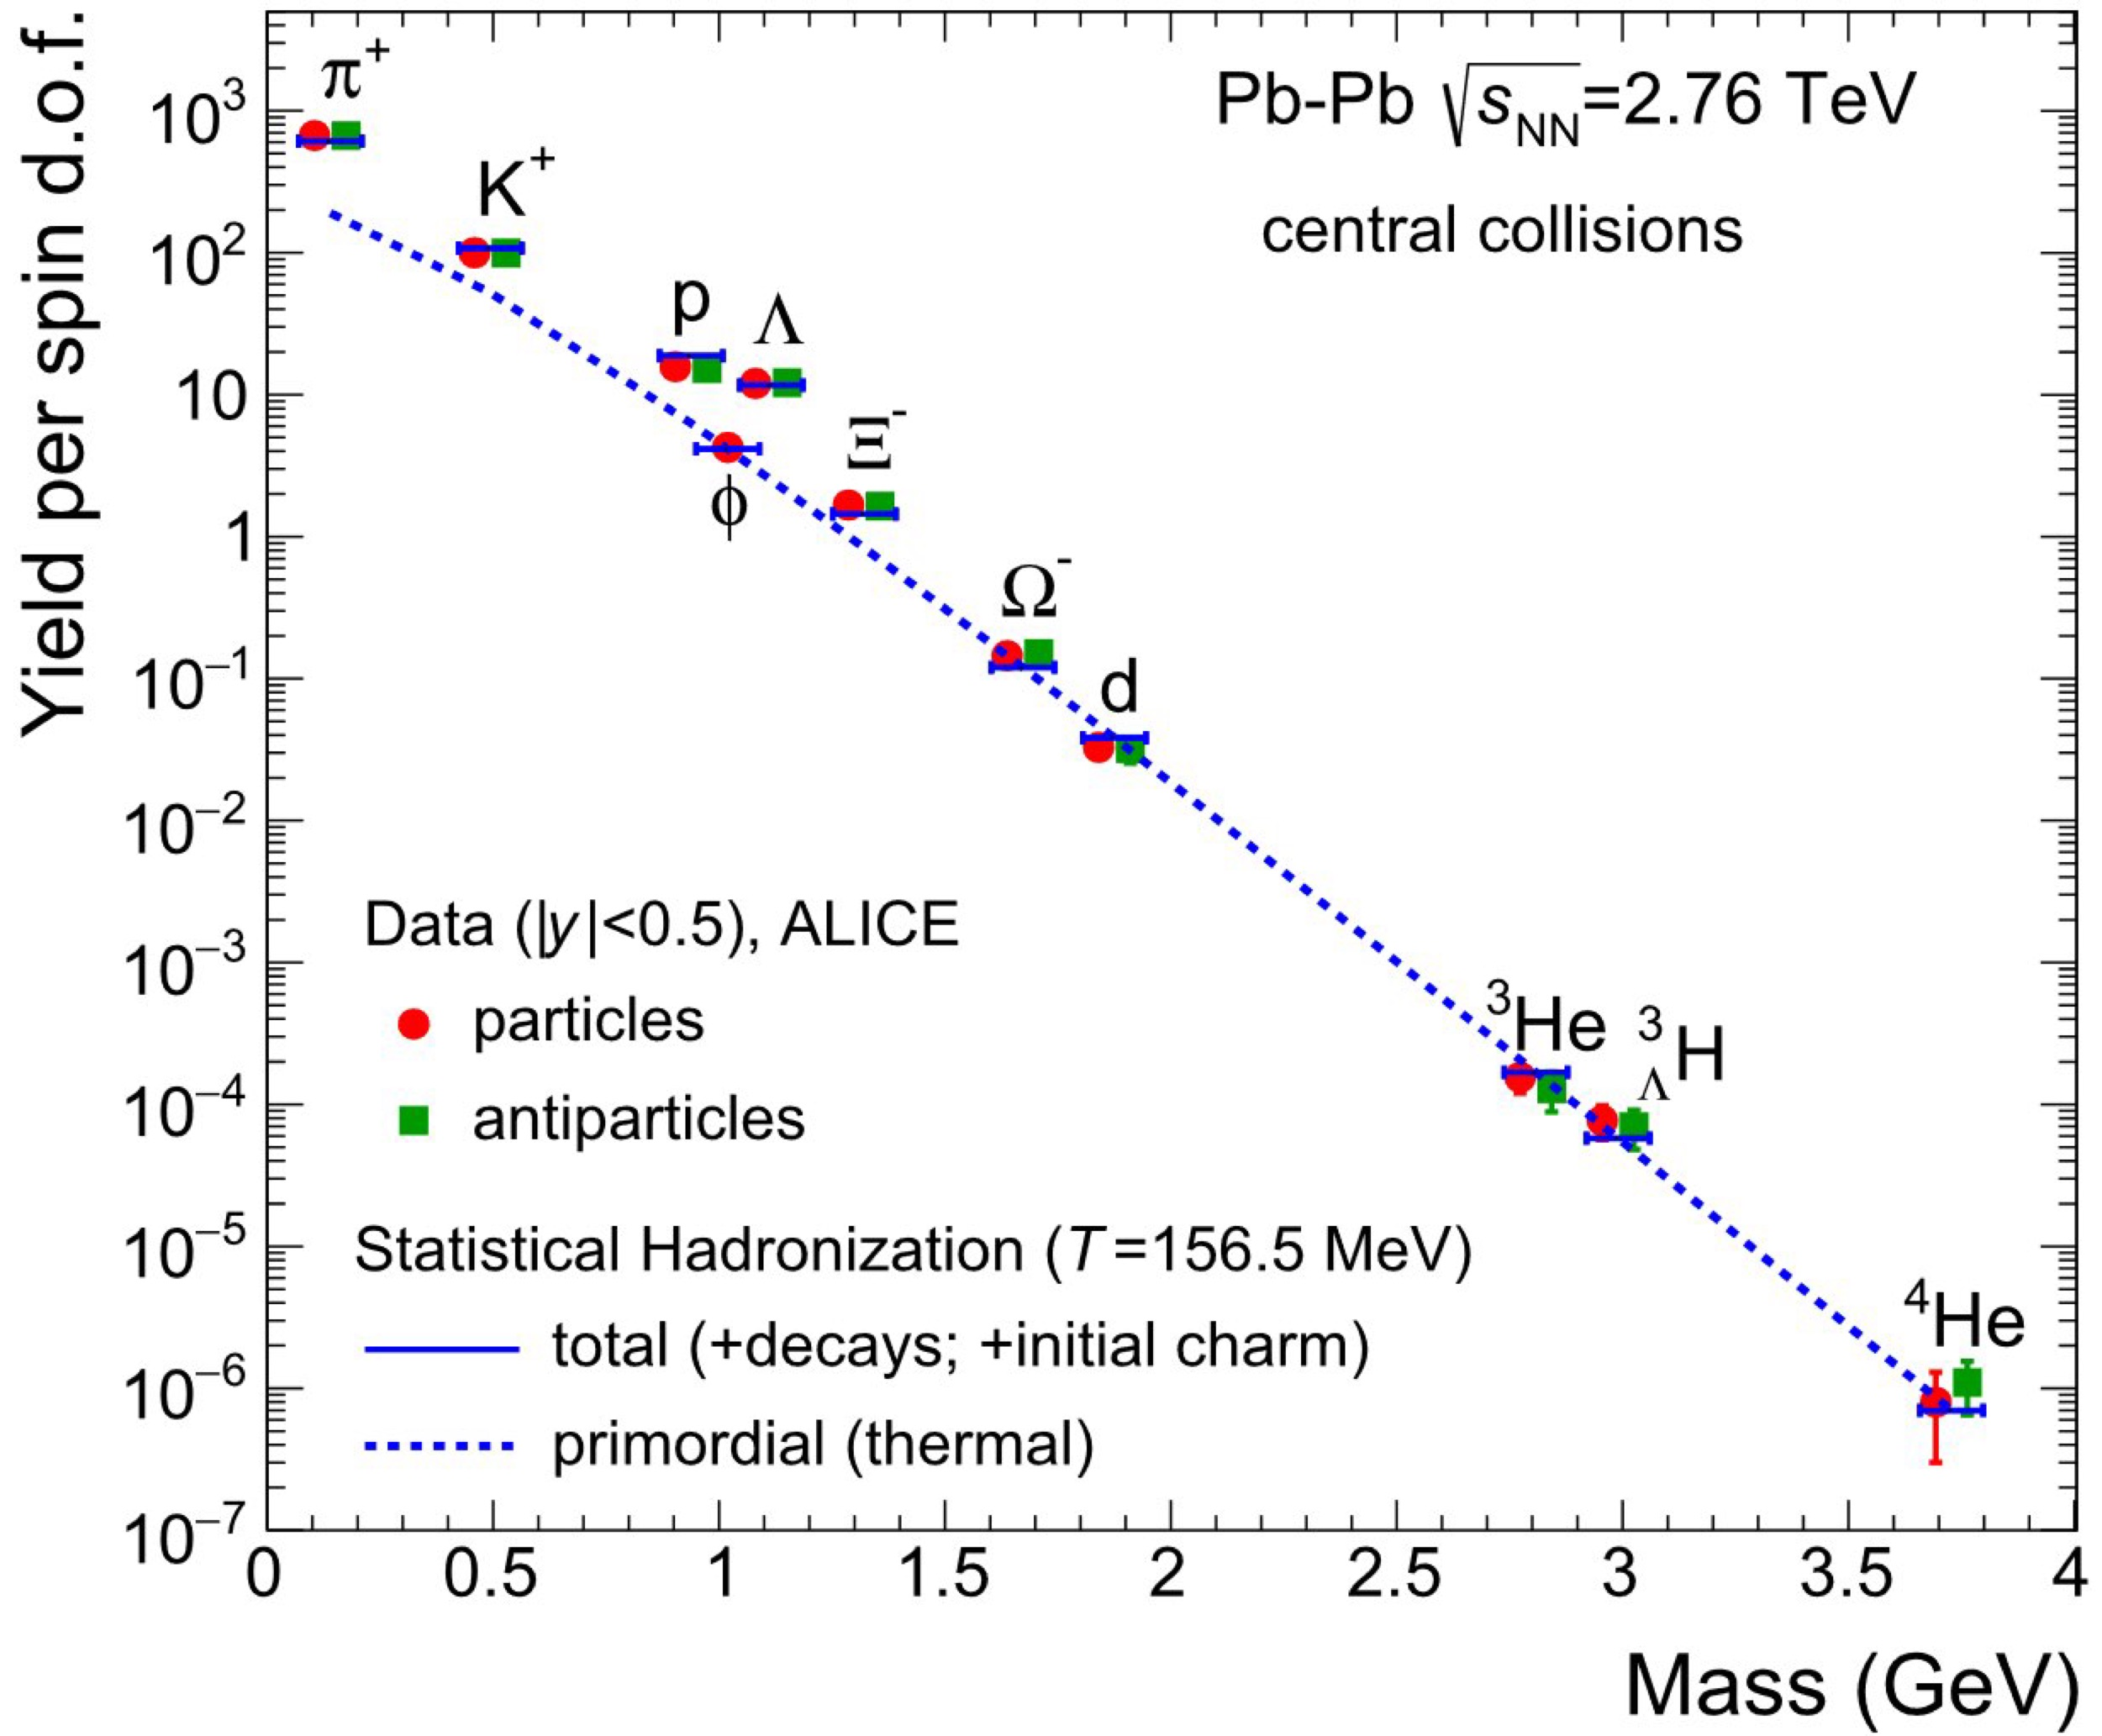
\includegraphics[width=0.6\linewidth]{image/2-modelli/mass_yield.jpg}
    \captionwithsource{(Linea tratteggiata) Variazione della produzione delle (anti)particelle rispetto alla rapidità (normalizzato  degenerazione di spin) in funzione della massa della particella, in confronto con i dati di ALICE.}{\cite{mass_yield}}
    \label{fig:mass_yield}
\end{figure}
    \item Predizioni del rapporto tra materia e antimateria in funzione dell'energia della coppia di nucleoni.
    Si può osservare come per valori piccoli dell'energia di collisione ($\sim$ 100 GeV), il potenziale barionico, una misura del rapporto materia-antimateria, assuma valori alti, per poi tendere a zero con l'aumentare dell'energia del sistema.
    Questo è compatibile con ciò che si osserva in LHC (\autoref{fig:matter_antimatter}) in cui la simmetria tra materia e antimateria è praticamente ottenuta \cite{Tawfik_2011_matter_antimatter}.
\end{itemize}
\begin{figure}[htbp]
    \centering
    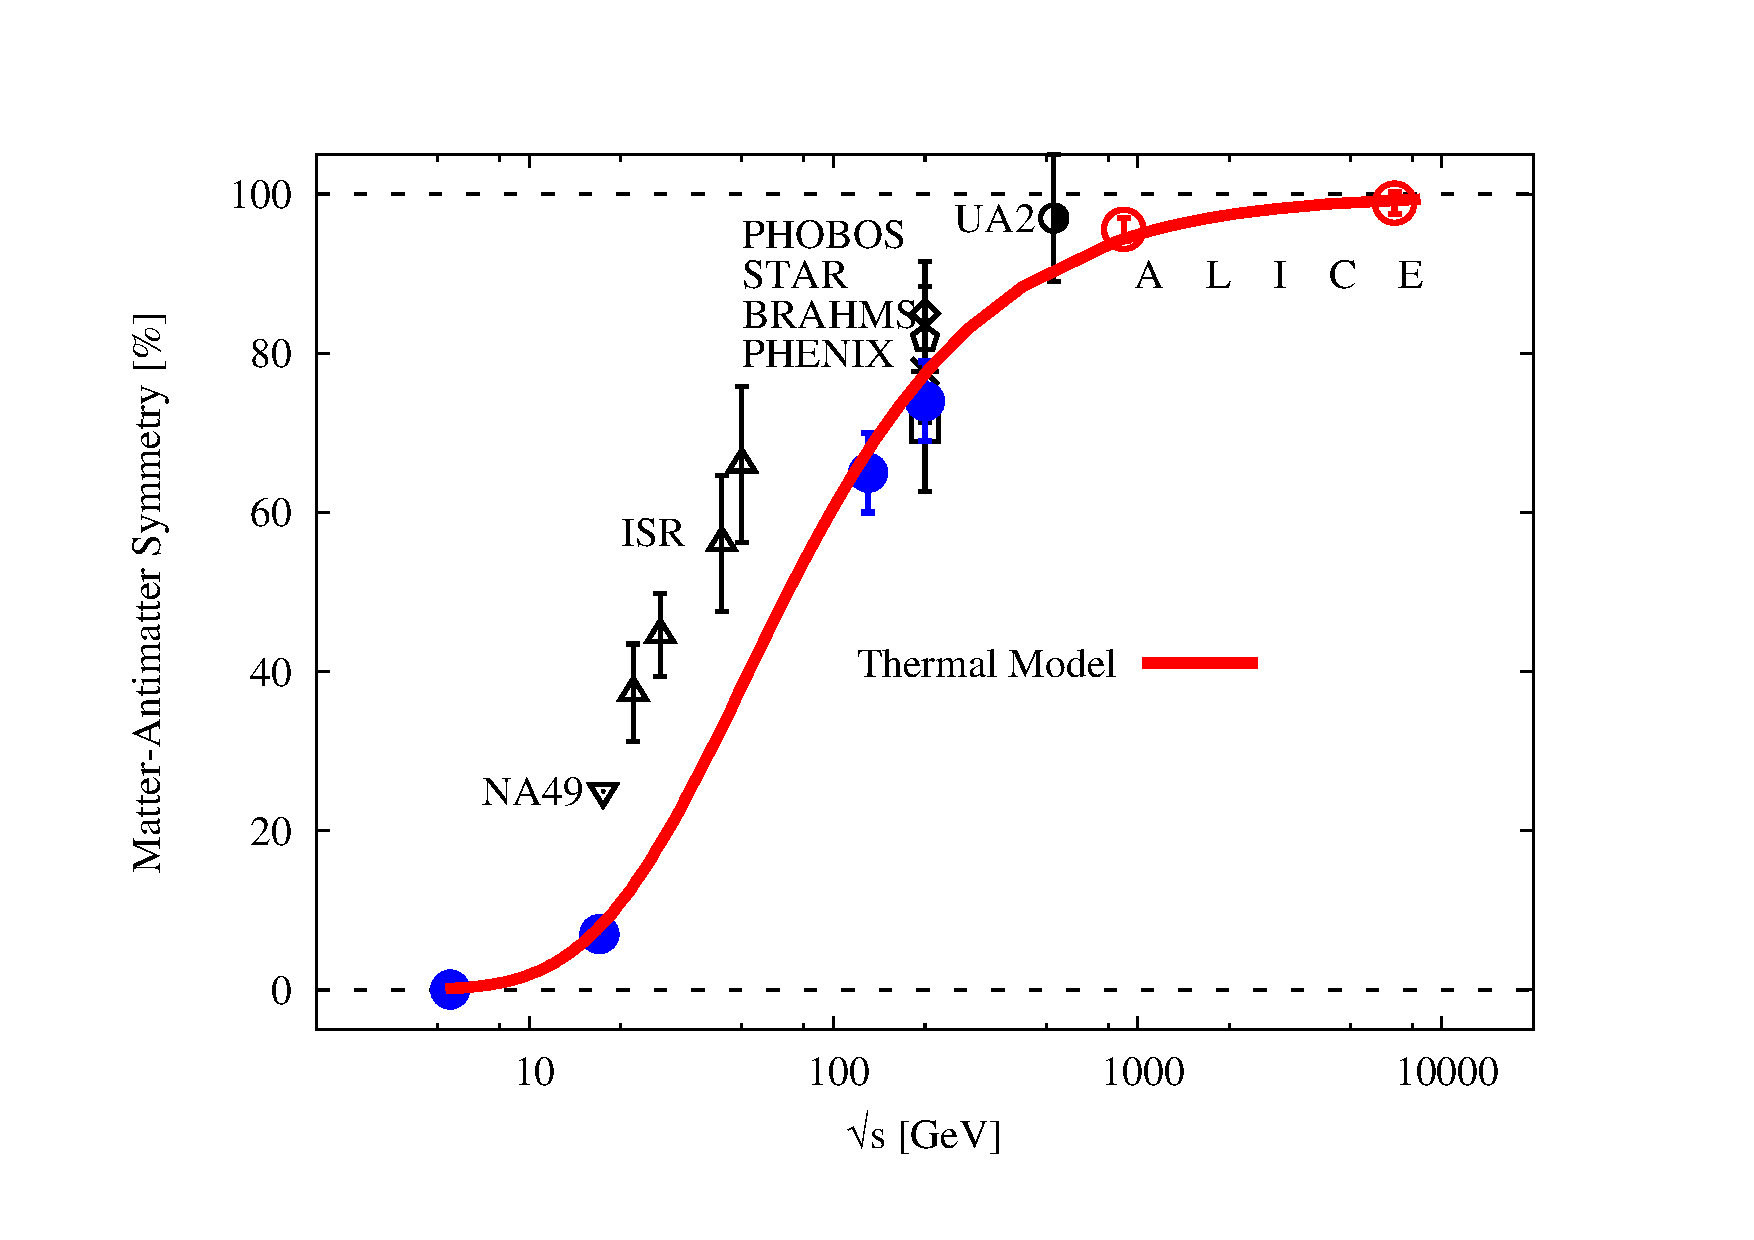
\includegraphics[width=0.8\linewidth]{image/2-modelli/antiPP_Alice2010_2.pdf}
    \captionwithsource{Rapporti di ${\bar{p}}/p$ in funzione dell'energia del centro di massa $\sqrt{s}$. I simboli vuoti indicano i risultati da vari esperimenti di collisioni pp, mentre i simboli pieni rappresentano quelli da collisioni di ioni pesanti. La curva nera rappresenta le previsioni del modello termico sul rapporto $\bar p/p$ del SMH.}{\cite{Tawfik_2011_matter_antimatter}}
    \label{fig:matter_antimatter}
\end{figure}
\section{Confronto del modello di coalescenza con il CSM}
In questa sezione si esegue un confronto tra il modello di coalescenza e il modello di adronizzazione statistica canonica.
Per far ciò confrontiamo i modelli teorici con dati sperimentali riguardo alle misure di rapporti di produzione tra nuclei e protoni in funzione della molteplicità \cite{alice_2022_coal_formula}.
Più specificatamente si vanno a considerare i rapporti $(D+\bar D)/(p + \bar p)$ e $(^3\text{He} + ^3\overline{\text{He}})/(p+\bar p)$.
I grafici prodotti sono riportati in \autoref{fig:NoPvsMult}.
Per le previsioni del CSM utilizza il pacchetto software del \ttbox{Thermal-FIST} \cite{Vovchenko_2019_thermal_FIST}, utilizzando dei volumi di correlazione $V_C$ tra 1 e 3 unità di rapidità.
Invece, per il modello di coalescenza si utilizza l'implementazione effettuata in \cite{Sun_2019_coal_model}.
È importante notare che si sono utilizzati due modelli di coalescenza per il nucleo di (anti)$^{3}{\rm He}$: il modello di coalescenza a tre corpi, in cui si assume la formazione del nucleo a partire dalla vicinanza di due protoni e di un neutrone; il modello a due corpi, in cui si assume la formazione del nucleo a partire da un (anti)deuterone e un (anti)neutrone. 
\begin{figure}[h]
    \centering
    \begin{subfigure}{.49\textwidth}
    \centering
        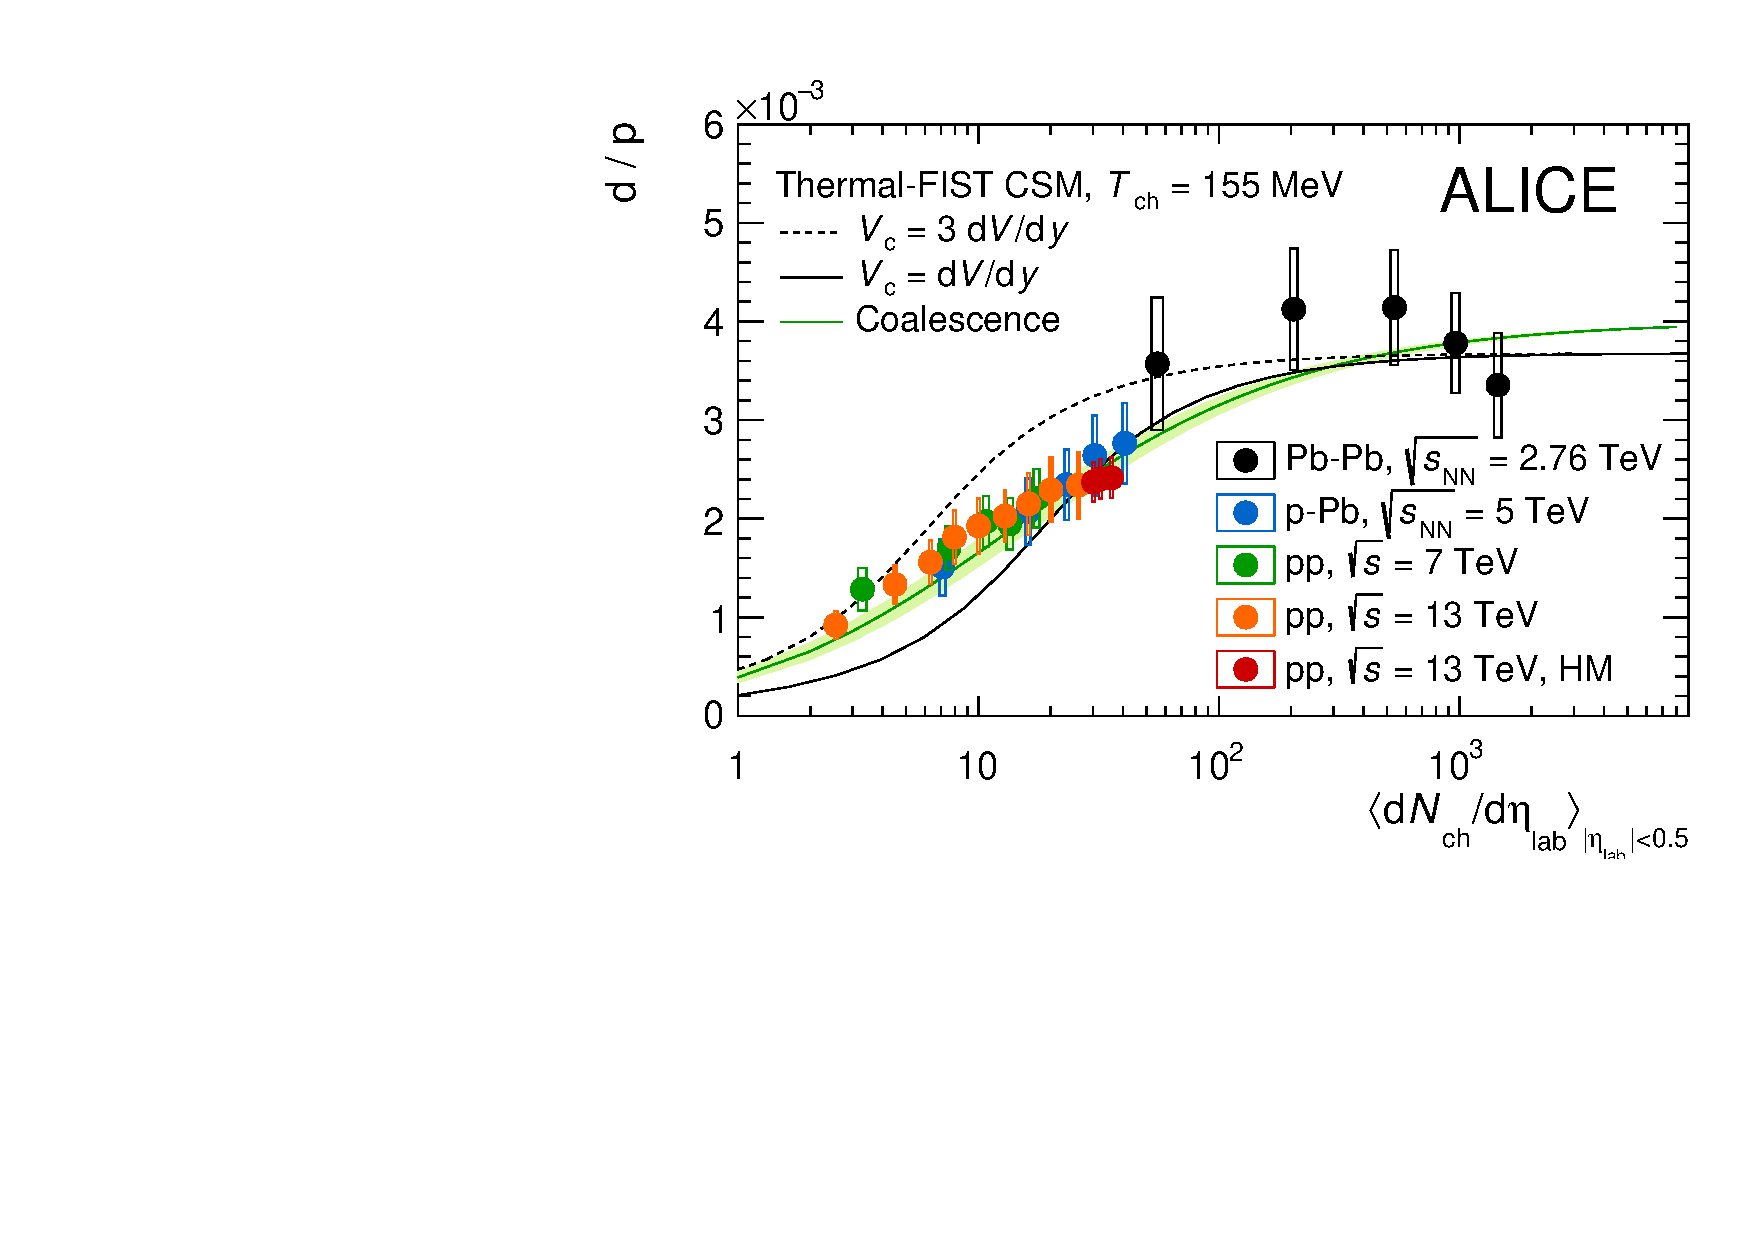
\includegraphics[width=\textwidth]{image/2-modelli/cDoPvsMult.pdf}
        \caption{$(D+\bar D)/(p + \bar p)$}
        \label{fig:cDoPvsMult}
    \end{subfigure}
    %\hspace{1cm}
    \begin{subfigure}{.49\textwidth}
        \centering
        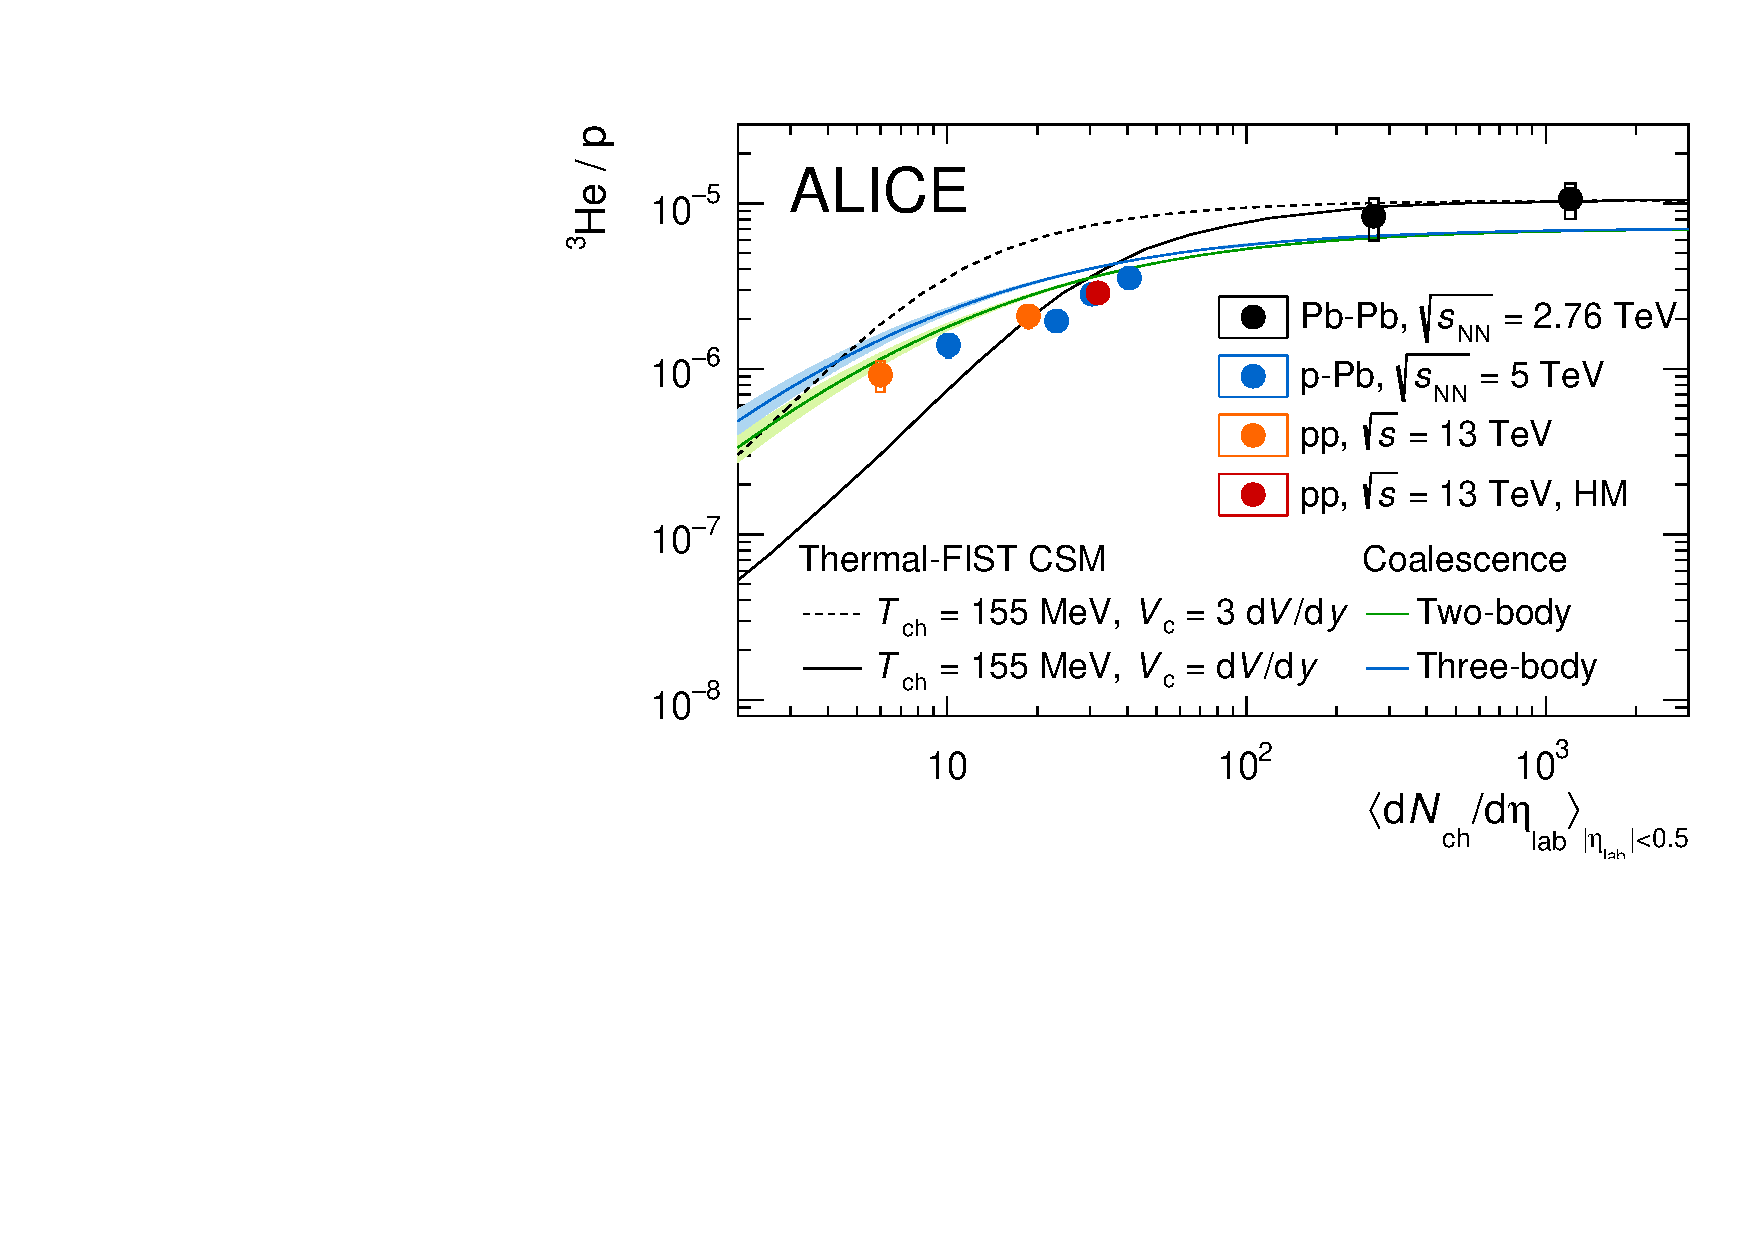
\includegraphics[width=\textwidth]{image/2-modelli/cHEoPvsMult.pdf}
        \caption{$(^3\text{He} + ^3\overline{\text{He}})/(p+\bar p)$}
        \label{fig:cHEoPvsMult}
    \end{subfigure}
    \captionwithsource{Misure (punti colorati) dei rapporti tra la produzione dei nuclei e protoni in funzione della molteplicità per \emph{\rmfamily (a)} (anti)deuteroni e \emph{\rmfamily (b)} (anti)nuclei di $^3\text{He}$. Le linee nere continue e tratteggiate rappresentano le previsioni del \emph{\ttbox{Thermal-FIST}} CSM.
    "$d/p$" indica $(D+\bar D)/(p + \bar p)$ e "$^3\text{He}/p$" indica $(^3\text{He} + ^3\overline{\text{He}})/(p+\bar p)$.
    In \emph{\rmfamily (a)} la linea verde rappresenta il modello di coalescenza, in \emph{\rmfamily (b)} la linea verde e blu rappresentano rispettivamente il modello di coalescenza a due corpi e a tre corpi.}{\cite{alice_2022_coal_formula}} 
    \label{fig:NoPvsMult}
\end{figure}

Per quanto riguarda le misure sperimentali, esse sono consistenti con esperimenti effettuati in passato \cite{Adam_2016_a1, 2017_a2, Acharya_2018_a3}: gli andamenti dei due rapporti aumentano con l'aumentare della molteplicità e i valori si saturano ad alte molteplicità.
Per quanto riguarda invece le previsioni teoriche, solamente il modello di coalescenza sembra essere qualitativamente in accordo con i dati, per entrambi i rapporti.
In particolare per $D/p$, il modello di coalescenza riesce a riprodurre fedelmente i dati per tutto l'intervallo della molteplicità, mentre per $^3\text{He}$ abbiamo una migliore concordanza del modello di coalescenza a due corpi nelle regioni a bassa bassa molteplicità, mentre ad alte molteplicità (come per le misure delle collisioni Pb-Pb) si ha un discostamento maggiore.
Il modello statistico canonico fornisce invece un andamento più qualitativo per molteplicità più basse, mentre ha un andamento consistente con i dati nel regime del gran-canonico (ossia nelle molteplicità caratterizzate dagli urti Pb-Pb).
\section{PYTHIA 8.3}
\pythiaa{} \cite{pythia8300} è un generatore Monte Carlo utilizzato principalmente per la generazione di eventi di collisione di particelle nella fisica delle alte energie. 
Più in particolare esso riesce a riprodurre processi QCD utilizzando sia implementazioni teoriche che fenomenologiche, dove i parametri sono determinati a partire da dati sperimentali. 
L'utilizzo di \pythiaa{} può essere utile in molteplici campi, per esempio la maggior parte della base degli utenti proviene dalle grandi collaborazioni di LHC, ma anche in fisica astroparticellare oppure nucleare.

Per evento di collisione si intende l'insieme degli avvenimenti che comprendono le particelle iniziali, le particelle finali e tutte le particelle e risonanze intermedie.
La ripetizione nella generazione di questi eventi deve essere necessariamente resa casuale, data l'imprevedibilità dei processi quanto-meccanici.
La generazione dipende da parametri che vengono impostati nel software che possono essere modificati a piacimento dall'utente a seconda delle proprie esigenze.

\subsection{Struttura del programma}
% struttura di programma
In un vero evento di collisione di particelle vi sono numerosi processi QCD, QED e altri che sono noti per essere molto complessi, perciò è logico andare a ordinarli e raggrupparli secondo un criterio temporale o in termini di energie.
Per esempio in \cite{pythia8300} si prende come esempio un evento $pp\to t\bar t$ e si ordinano gli eventi secondo una logica in termini dell'\textit{hardness} dei processi:
si parte con uno scattering inelastico di partoni, seguito dalla produzione di risonanze (bosoni deboli o quark top), con aggiunta di correzioni radiative.
Successivamente si hanno radiazioni dello stato iniziale (ISR), e dello stato finale (FSR), originati dal decadimento delle particelle iniziali e dalle risonanze rispettivamente.
Queste radiazioni sono sostanzialmente sciami (o cascate) di partoni.
Contestualmente a ciò vi sono interazioni multi-partoniche (MPI), ulteriori processi di scattering, in aggiunta ad altri processi QCD che esulano dalla trattazione di questa tesi. 
Infine verso la fine del processo si formano gli adroni stabili a partire da decadimenti dei partoni instabili.
Una rappresentazione grafica di tutti questi processi è riportata in \autoref{fig:eventSchematic}.

\begin{figure}[htpb]
\centering % 73% + 27%
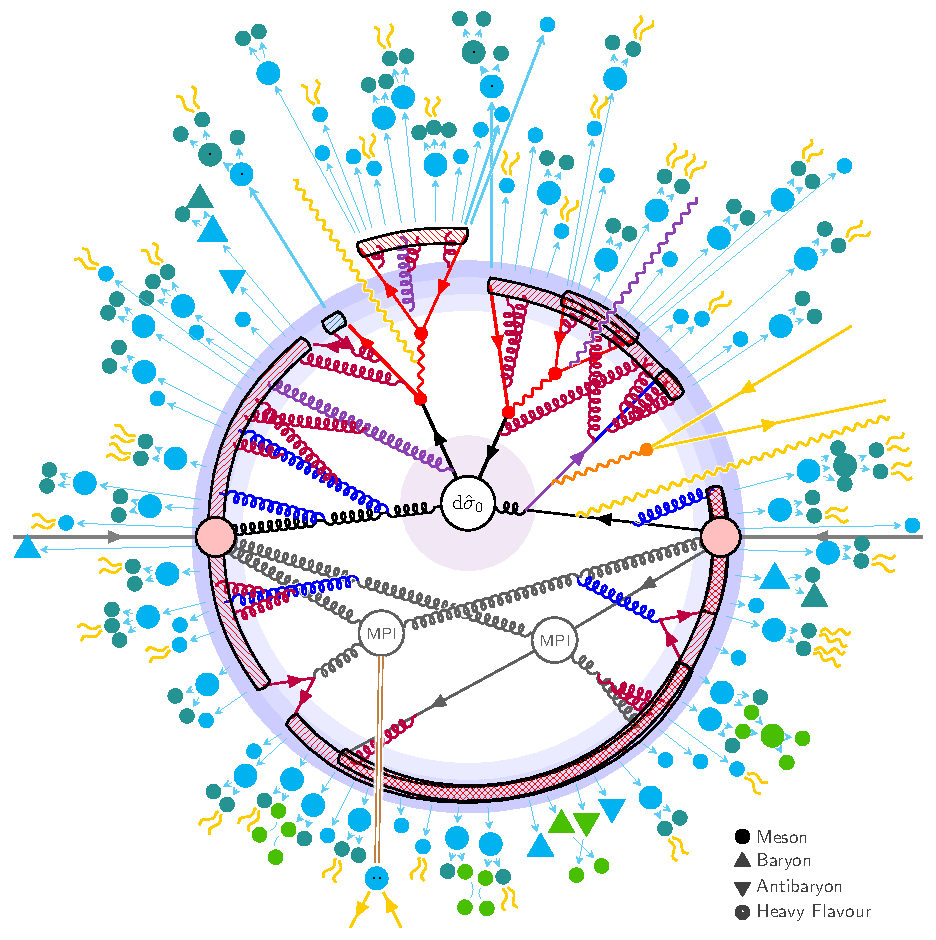
\includegraphics[width=0.73\textwidth]{image/2-modelli/event.pdf}%
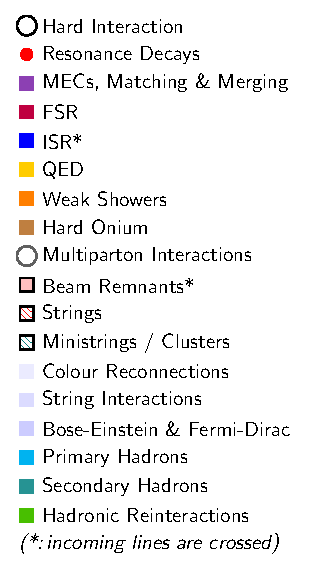
\includegraphics[width=0.27\textwidth]{image/2-modelli/eventLegend.pdf}
\captionwithsource{Schematica (semplificata) di un evento $pp\to t\bar t$ nel modello di \emph{\pythiaa{}}.
Le particelle entranti sono rappresentate dalle linee grigie esterne a metà altezza.  
\label{fig:eventSchematic}}{\cite{pythia8300}}
\end{figure}

\pythiaa{}, ispirandosi a questo modo di trattare un evento, è suddivisa in tre parti principali:
\begin{enumerate}
    \item \emph{livello di processo}, corrispettivo del processo di scattering duro, dove vengono prodotte anche le risonanze;
    \item \emph{livello di partoni}, dove vengono gestite le ISR e le FSR tramite l'implementazione di modelli di sciami partonici, le MPI e varie correzioni QCD;
    \item \emph{livello di adroni}, durante la quale viene gestita l'adronizzazione in senso stretto, tramite decadimenti di adroni e risonanze instabili e altri processi più tecnici.
\end{enumerate}
Ovviamente questi livelli non sono gestiti in maniera totalmente separata, ma vi è un numero significativo di oggetti condivisi da un livello all'altro.

% https://amzn.eu/d/6InjjKU per giovanni

\subsection{Gli algoritmi di generazione}
%%%%%%%%%%
Gli algoritmi di generazione in \pythiaa{} si basano su numeri pseudo-casuali campionati da distribuzioni di probabilità, simulando la natura stocastica degli eventi reali nelle collisioni di particelle.
In seguito vengono elencate le due principali utilizzate nel programma.
\begin{itemize}
    \item \emph{Algoritmo di veto}, il principale algoritmo di \pythiaa{} per simulare processi come decadimenti radiativi, cascate partoniche o interazioni multi-partoniche (MPI).
    Il suo funzionamento è semplice: partendo da una funzione di prova che sovrastima la distribuzione di probabilità desiderata, vengono generati dei campioni e viene deciso se sono conformi alla probabilità voluta, e in base a ciò viene deciso se la funzione di prova sia accettabile o se vi sia bisogno di ripetere questo step.
    Esistono inoltre anche varianti di questo algoritmo;
    % aggiungere altro se serve
    \item vi sono algoritmi per la distribuzione uniforme della quantità di moto nello spazio delle fasi.
    Nel caso di due particelle questo è triviale, in quanto è sufficiente emetterle in direzioni opposte nello spazio dei momenti.
    Mentre per tre o più particelle prodotte vengono utilizzate principalmente \emph{M-generator} e \emph{RAMBO}.
    Quest'ultimo è la migliore scelta per i prodotti senza massa (o massa trascurabile).
    \textit{M-generator} funziona scomponendo un processo di produzione  multiparticellare in produzione di 2 particelle.
    Per esempio un processo $0\to1234$ viene scomposto in $0\to(123) + 4$ e così via.
\end{itemize}
In generale, per ogni processo in \pythiaa{} è spesso implementata una forma derivata da uno di questi due principali algoritmi.   

\subsection{Formazione di deuteroni in PYTHIA} \label{ch:pythia_deuteron}
\pythiaa{} supporta la produzione deuteronica tramite due modelli di produzione, ovvero il modello di coalescenza e il modello di sezioni d'urto efficaci, chiamato anche modello di Dal-Raklev \cite{Dal_2015}, con quest'ultimo come opzione predefinita di \pythiaa{}.
Si noti come in questo paragrafo, per evitare ripetizioni, si tratterà solamente della produzione dei deuteroni, invece la trattazione degli antideuteroni è equivalente nel momento in cui si considerano le antiparticelle corrispettive.

\subsubsection{Modello di coalescenza}
Il modello di coalescenza, come già detto in precedenza, prevede la formazione di un deuterone nel momento in cui un protone e un neutrone sono sufficientemente vicini nello spazio delle fasi.
L'implementazione di questo modello in \pythiaa{} è effettuata in questo modo: vengono prese in considerazione tutte le coppie possibili di protoni e neutroni $p-n$ e si considera per ognuna di esse il modulo della differenza della loro quantità di moto (calcolato nel sistema di centro di massa di ognuna coppia)
\begin{equation}\label{eq:momentum_difference_k}
    k = |\vec p_p - \vec p_n|
\end{equation} 
Si determina la formazione del deuterone nel momento in cui $k<p_0$, con $p_0$ un parametro da determinare sperimentalmente.
È importante notare come non vi sia considerazione delle coordinate spaziali.
Un altro elemento da tenere in conto è la violazione energetica della coalescenza, ossia che il processo $pn\to D$ non è possibile se nello stato finale non vi sia un'altra particella.
Per ovviare a questo problema si considera al posto di questa reazione la cattura radiativa, ovvero $pn\to \gamma D$, in quanto provvede a fornire un'approssimazione ragionevole del processo.
Per esprimere la probabilità di formazione del deuterone in funzione di $k$ in modo compatto si può farlo nel seguente modo
\begin{equation}
    P(k) = \theta(p_0-k)
\end{equation}
con $\theta(k)$ la funzione gradino di Heaviside.

\subsubsection{Modello di sezioni d'urto efficaci}
Nel modello di sezioni d'urto efficaci si punta a descrivere la formazione dei deuteroni da un punto di vista probabilistico, di fatto considerando la probabilità di formazione $P_\text{processo}(k)$ direttamente proporzionale alla sezione d'urto differenziale del processo $\sigma_\text{processo}(k)$
\begin{gather}
    P_\text{processo}(k) \propto \dfrac{d\sigma_\text{processo}(k)}{dk} \\
    \implies P_\text{processo}(k) = \dfrac1{\sigma_0}\dfrac{d\sigma_\text{processo}(k)}{dk} 
\end{gather}
con $k$ la grandezza definita dell'\autoref{eq:momentum_difference_k} e $\sigma _0$ una costante di proporzionalità da determinare sperimentalmente, analogo di $p_0$.
L'obiettivo del modello di sezioni d'urto efficaci è anche quello di uniformare questo parametro in modo che sia costante in tutti gli esperimenti, al contrario di $p_0$ che assume valori diversi in esperimenti diversi. 

A differenza del modello di coalescenza, in questo modello non si considera solamente la reazione della cattura radiattiva, ma se ne considerano molteplici.
I canali di produzione dei deuteroni sono riportati in \autoref{tab:canali}.

\begin{table}[H]
    \centering
    \begin{tabular}{clcl}
    \hline \hline
    1) & $pn \to \gamma D$ & 5) & $pp \to \pi^+ D$\\
    2) & $pn \to \pi^0 D$ & 6) & $pp \to \pi^+\pi^0 D$\\
    3) & $pn \to \pi^-\pi^+ D$ & 7) & $nn \to \pi^- D$\\
    4) & $pn \to \pi^0\pi^0 D$ & 8) & $nn \to \pi^-\pi^0 D$\\
    \hline\hline
    \end{tabular}
    \caption{I canali di produzione dei deuteroni considerati nel modello di sezione d'urto. Per ottenere i canali dell'antideuterone è sufficiente considerare le antiparticelle.}
    \label{tab:canali}
\end{table}
Ognuno di questi canali ha una propria probabilità di formazione, determinata non più come una semplice distribuzione uniforme con cut-off come nel modello di coalescenza, ma determinata da fit di dati sperimentali sullo scattering differenziale di nucleoni.

Le possibili funzioni di sezioni d'urto differenziali ${d\sigma_\text{processo}(k)}/{dk}$ sono tre:
\begin{itemize}
    \item Per $pn\to\gamma D$ è parametrizzato da un polinomio sotto a un valore $a_0$ di $k$, altrimenti da un andamento esponenziale
    \begin{equation}
        \dfrac{d\sigma(k)}{dk} =
        \begin{cases}
            \displaystyle\sum_{i=1}^{12}a_ik^{i-2} & k<a_0 \\
            e^{-c_{13}k - c_{14}k} & k>a_0
        \end{cases}
    \end{equation}
    Si assume inoltre che per $k<0.1$ GeV la sezione d'urto differenziale sia fissata al valore di $k=0.1$ GeV.

    \item Per processi che coinvolgono la formazione di un pione e di un deuterone si assume la seguente forma della sezione d'urto differenziale
    \begin{equation}
        \dfrac{d\sigma(q)}{dq} = \dfrac{c_0\ q^{c_1}}{(c_2-e^{c_3 q})^2 + c_4}
    \end{equation}
    con $q = |\vec p_\pi|/m_\pi$, con $\vec p_\pi$ la quantità di moto del pione nel centro di massa e $m_\pi$ la massa del pione.

    \item Infine per i processi di formazione di 3 corpi la sezione d'urto differenziale è parametrizzata nel seguente modo
    \begin{equation}
        \dfrac{d\sigma(k)}{dk} = \sum_{i=0}\dfrac{c_{5i}\ k^{c_{1+5i}}}{(c_{2 + 5i}-e^{c_{3 + 5i} k})^2 + c_{4 + 5i}}
    \end{equation}
\end{itemize}
La giustificazione dell'utilizzo di queste forme delle sezioni d'urto è reperibile in \cite{Dal_2015}.\\

I valori dei parametri di coalescenza ($p_0$) e di Dal-Raklev sono già stati determinati eseguendo fit ai dati sperimentali e possono essere reperiti in \cite{Dal_2015}.
In \pythiaa{}, come è già stato detto, il modello predefinito è il modello di sezioni d'urto efficaci.
Il parametro $\sigma_0$, o meglio $1/\sigma_0$, è un parametro importante perché determina il numero di deuteroni prodotti in tutti i canali di produzione. 
Tuttavia, per ragioni pratiche, in \pythiaa{} il parametro $1/\sigma_0$ è incorporato in un altro parametro, ovvero \ttbox{DeuteronProduction:norm}, che per semplicità indicheremo con \ttbox{norm}, calcolato come 
\begin{equation}\label{eq:norm}
    \ttbox{norm} = \dfrac{1}{(1/\sigma_0)(d\sigma/dk)_\text{max}}
\end{equation}
con $(d\sigma/dk)_\text{max}$ il valore della sezione d'urto differenziale massima.
Il ruolo di questo parametro è simile a quello di $1/\sigma_0$, ossia quello di regolare il numero di (anti)deuteroni prodotti per tutti i canali. Più è alto il suo valore, minore è la produzione, e viceversa.\\

Usando i parametri della tabella VI di \cite{Dal_2015} è possibile ricavare il valore massimo della sezione d'urto differenziale che è di circa $3.18$ mb.
Perciò ora per ottenere il valore di \ttbox{norm} è sufficiente conoscere il valore di $1/\sigma_0$.
Tuttavia, la determinazione di questo parametro è problematica perché varia in base all'energia del centro di massa $\sqrt s$, e in \cite{Dal_2015} sono stati ottenuti i valori di $1/\sigma_0$ e di $p_0$ che vengono riportati nella tabella VIII in \cite{Dal_2015}, in base a fit effettuati sui dati di ALICE.
Questi valori sono riportati per convenienza in \autoref{tab:valori_p0_1sigma0}.
\begin{table}[H]
    \centering
    \begin{tabular}{||c||c|c||c|c||}
    \hline \hline
    & \multicolumn{2}{c||}{$p_0$ [\si{MeV}]} & \multicolumn{2}{c||}{$1/\sigma_0$ [\si{barn^{-1}}]}\\
    \hline
    \textsc{energia} & \textsc{deuteroni} & \textsc{antideut.} & \textsc{deuteroni} & \textsc{antideut.} \\ 
    \hline
    0.9 TeV & 201 & 201 & 3.58 & 3.63\\
    2.76 TeV & 194 & 196 & 2.93 & 2.88\\
    7 TeV & 194 & 195 & 2.63 & 2.58\\
    \hline\hline
    \end{tabular}
    \captionwithsource{I valori dei parametri $p_0$ e $1/\sigma_0$ alle energie riportate. Per \emph{\rmfamily\textsc{energia}} si intende l'energia  del centro di massa $\sqrt s$.}{\cite{Dal_2015}}
    \label{tab:valori_p0_1sigma0}
\end{table}
\pythiaa{} utilizza il parametro \ttbox{norm} considerando esclusivamente il valore di $1/\sigma_0$ a 7 \si{TeV} dei deuteroni, quindi, utilizzando l'\autoref{eq:norm}, si ha che $\ttbox{norm} = 119.6$.

%%%%%%%%%%%%%%%%%%%%%%%%%%%%%%%%%%%%%%%%%%%%%%%%%%%%%
\chapter{Risultati e discussione}\label{ch:risultati}

In questo capitolo viene mostrato il lavoro centrale di questa tesi. Più in particolare verrà mostrata la metodologia utilizzata nel contesto di lavoro di \ttbox{PYTHIA 8.3}, ossia come  viene impostata la generazione gli eventi.
Successivamente verranno mostrati il confronto dei dati sperimentali di ALICE con le simulazioni, quali sono i contributi maggiori dei canali di produzione dei (anti)deuteroni e il confronto tra il modello di coalescenza e il modello di sezioni d'urto efficaci.
Dopodiché verrà mostrato come è stata effettuata l'ottimizzazione dei parametri di simulazione, cercando di ripercorrere le modalità utilizzate per la ricerca del parametro ottimale.
Infine si esegue un confronto delle simulazioni con il modello predefinito e il modello ottimizzato.

%%%%%%%%%%%%%%%%%%%%%%%%%%%%%%%%%
\section{La generazione degli eventi}\label{ch:settings}
Per la produzione delle simulazioni sono stati generati 98 milioni di eventi.
% NJ qui si può considerare la notazione scientifica e dire 10e8, sono sempre 98 milioni? 
Per ogni evento si sono impostate le seguenti opzioni:
\begin{itemize}
    \item ogni evento è una collisione $pp$ con l'energia del centro di massa $\sqrt{s} = 13$ TeV;
    \item si è attivata la simulazione della posizione di vertici per i partoni \\ (\ttbox{PartonVertex:setVertex = on});
    \item si è attivata la generazione di vertici nella frammentazione, ossia la formazione di particelle a partire da partoni (\ttbox{Fragmentation:setVertices = on});
    \item si è applicato un particolare \textit{tuning} (ottimizzazione) dei parametri per la simulazione delle collisioni $pp$ (\ttbox{Tune:pp = 4}, con "4" che si riferisce a un set specifico di parametri ottimizzati per certe condizioni sperimentali);
    \item si sono disattivati i sottoprocessi che coinvolgono interazioni QCD con trasferimento di momento elevato (\ttbox{HardQCD:all = off});
    \item si sono disattivati anche i sottoprocessi che coinvolgono interazioni QCD con trasferimento di momento più piccolo (\ttbox{LowEnergyQCD:all = off});
    \item si sono abilitate le interazioni QCD soft inelastiche che sono sottoprocessi di bassa energia (\ttbox{SoftQCD:inelastic = on});
    \item si è attivata la produzione di deuteroni (\ttbox{HadronLevel:DeuteronProduction = on}).
\end{itemize}
In ogni evento vengono prodotte un certo numero di particelle, che possono includere protoni, neutroni, fotoni, deuteroni e altro, con le rispettive antiparticelle, e sono stati ottenuti gli spettri di produzione di (anti)protoni e (anti)deuteroni in funzione dell'impulso trasverso $p_t$, scartando le particelle con alta pseudo-rapidità (quindi se una particella possiede pseudo-rapidità $\eta > 0.5$, essa viene scartata).
% NJ Qui il taglio era su eta o y? Dovrebbe esser y 
Inoltre si è andato a osservare gli spettri dei deuteroni in funzione della quantità di moto trasversa nei vari canali di produzione.
Contestualmente all'esecuzione di \pythiaa{}, il riempimento degli istogrammi è stato effettuato tramite l'utilizzo del programma \ttbox{ROOT} sviluppato al CERN \cite{fons_rademakers_2020_3895855}.
%%%%%%%%%%%%%%%%%%%%%%%%%%%%%%%%%%%%%%%%%%%%
\section{Risultati con parametri predefiniti}\label{ch:default}
Come già anticipato nella \autoref{ch:pythia_deuteron}, un parametro importante nella produzione deuteronica è \ttbox{norm}, che nel caso predefinito assume il valore di 119.6.
Tuttavia questo valore è stato ottenuto considerando l'energia iniziale del centro di massa a $\sqrt{s} = 7$ TeV, a differenza del valore di $\sqrt s = 13$ TeV considerato in questa tesi.
Perciò è lecito aspettarsi, a partire da questa considerazione, che vi sia una discrepanza nella produzione di (anti)deuteroni tra le simulazioni e i dati reali.
Per confrontare i dati delle simulazioni con i dati sperimentali si sono considerate le misure effettuate da ALICE riguardanti collisioni $pp$ a rapidità centrali ($|y|<0.5$) con energia del centro di massa $\sqrt s = 13$ TeV.
I dati dei protoni e dei (anti)deuteroni utilizzati in questa tesi sono tratti rispettivamente da \cite{ALICE:2020jsh} e da \cite{ALICE:2020foi}.\\

\begin{figure}[htb]
    \centering
    \begin{subfigure}{.49\textwidth}
    \centering
        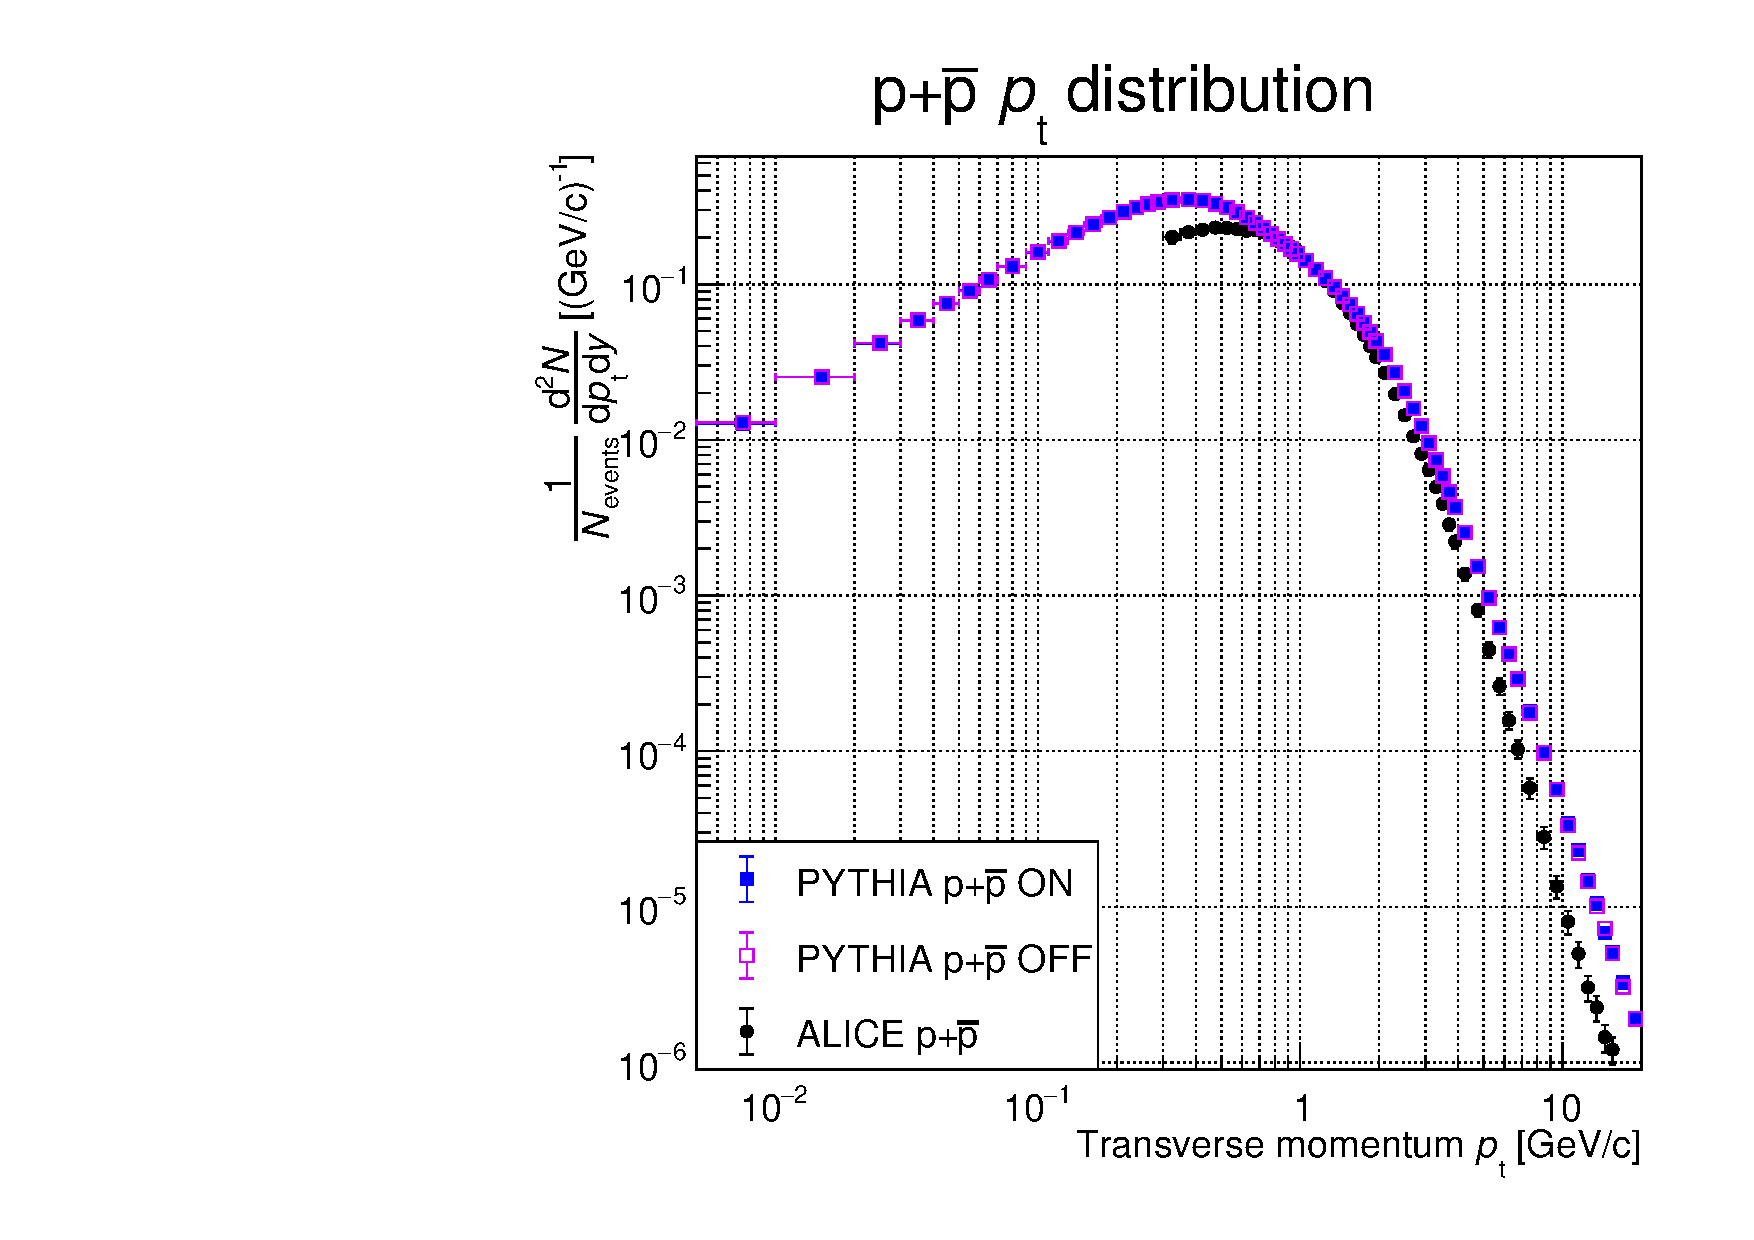
\includegraphics[width=\textwidth]{image/3-risultati/analyse/A/pp.pdf}
        \caption{}
        \label{fig:A_pp}
    \end{subfigure}
    %\hspace{1cm}
    \begin{subfigure}{.49\textwidth}
        \centering
        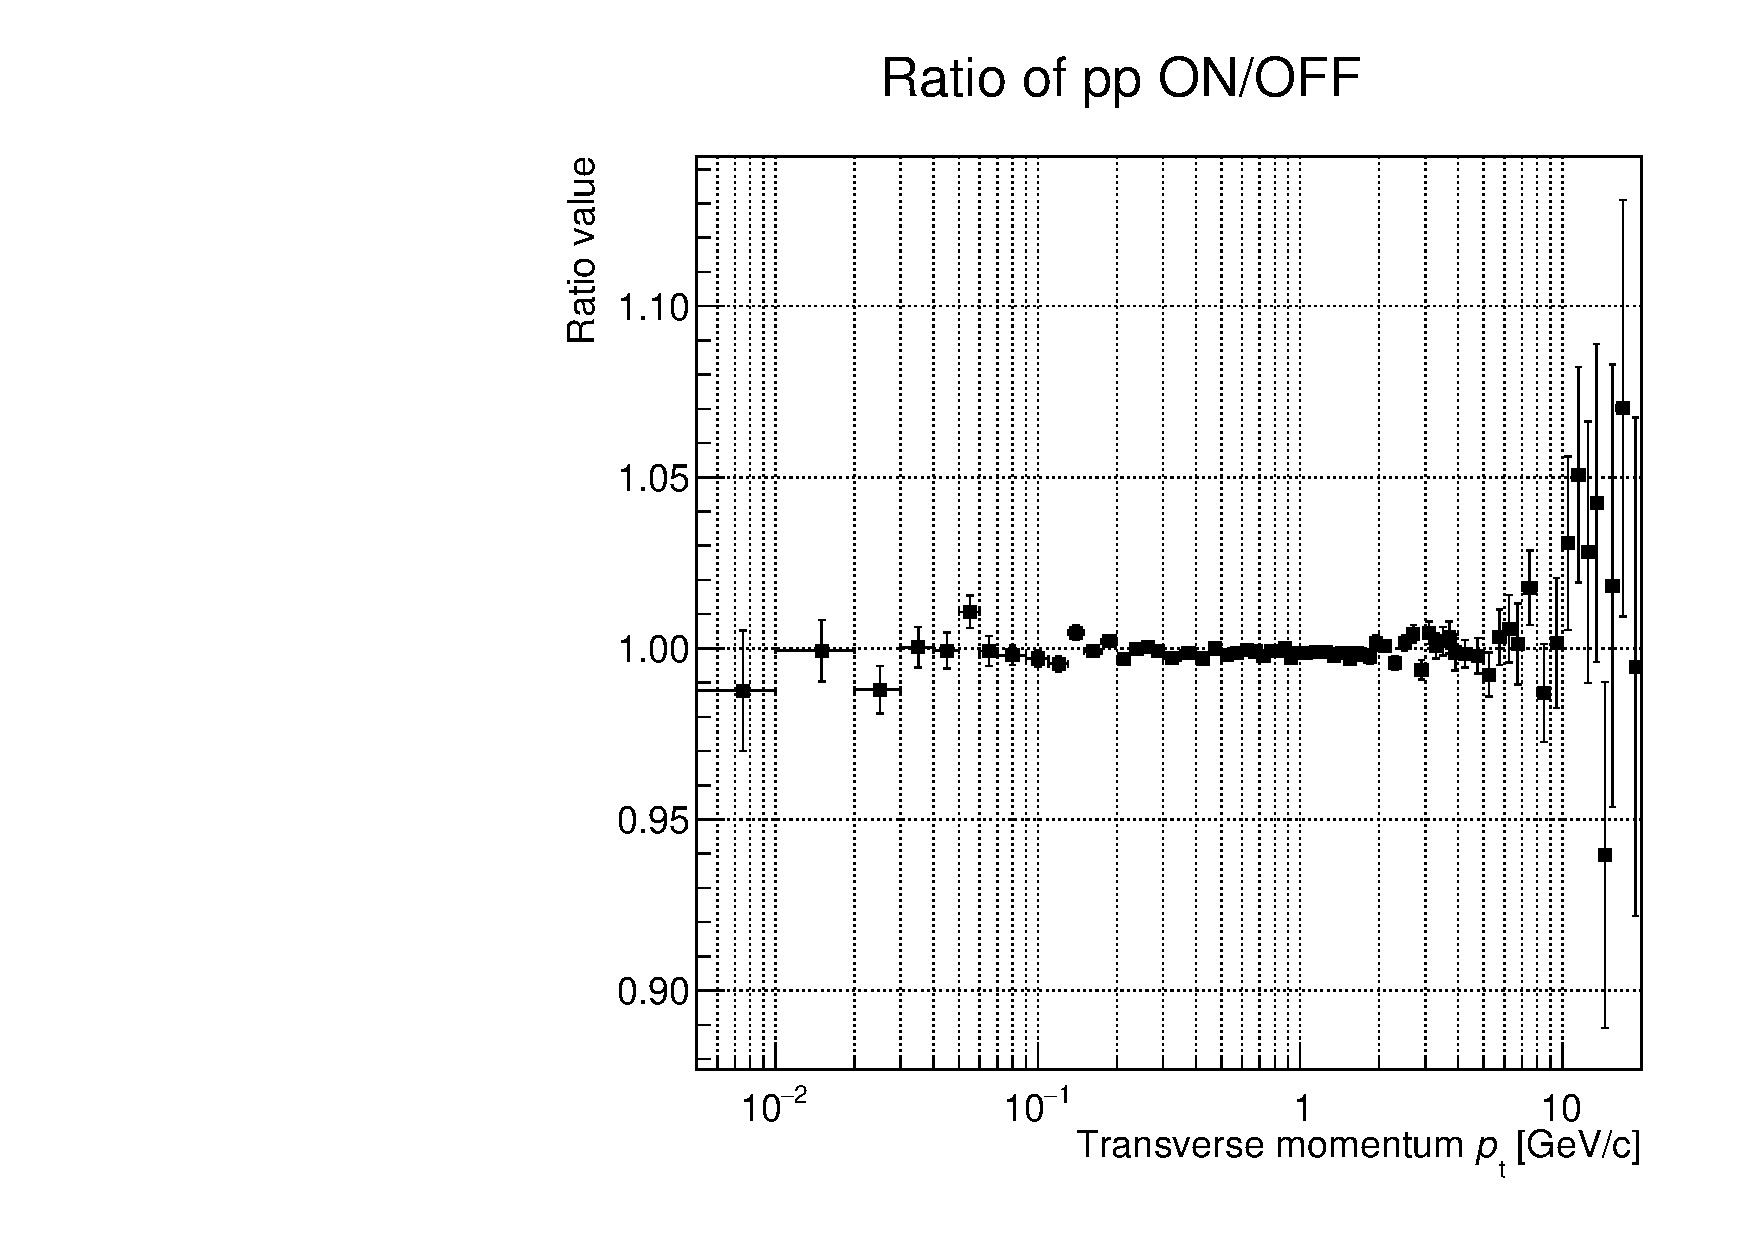
\includegraphics[width=\textwidth]{image/3-risultati/analyse/A/ratio_pp_ON_OFF.pdf}
        \caption{}
        \label{fig:A_ratio_pp_ON_OFF}
    \end{subfigure}
    \captionwithsource{\emph{\rmfamily (a)} Distribuzione dell'impulso trasverso di $p+\bar p$ con produzione deuteronica attivata e disattivata ("ON" e "OFF") in confronto con i dati sperimentali di ALICE ("ALICE"). \emph{\rmfamily (b)} Frazione della distribuzione dell'impulso trasverso di $p+\bar p$ con produzione deuteronica attivata e con produzione non attivata.}{\cite{ALICE:2020jsh}}
    \label{fig:A_pp_prod}
\end{figure}
Eseguendo la simulazione una volta con i parametri predefiniti e una volta con la produzione deuteronica disattivata (\ttbox{HadronLevel:DeuteronProduction = off}), otteniamo i vari spettri di produzione.
Ci si aspetta una piccola differenza tra il caso in cui la produzione di deuteroni è attivata e non, in particolare il numero di protoni dovrebbe essere leggermente minore in cui la produzione si attivata, visto che una parte di questi si ricombina per formare un deuterone.
Dalla \autoref{ch:objectives_alice} sappiamo che il numero di deuteroni prodotti deve essere circa 1000 volte inferiore al numero di protoni, per cui il rapporto tra numero di protoni con produzione (anti)deuteronica attivata e disattivata dovrebbe avvicinarsi al valore di 0.999.
\begin{figure}[htb]
    \centering
    \begin{subfigure}{.49\textwidth}
    \centering
        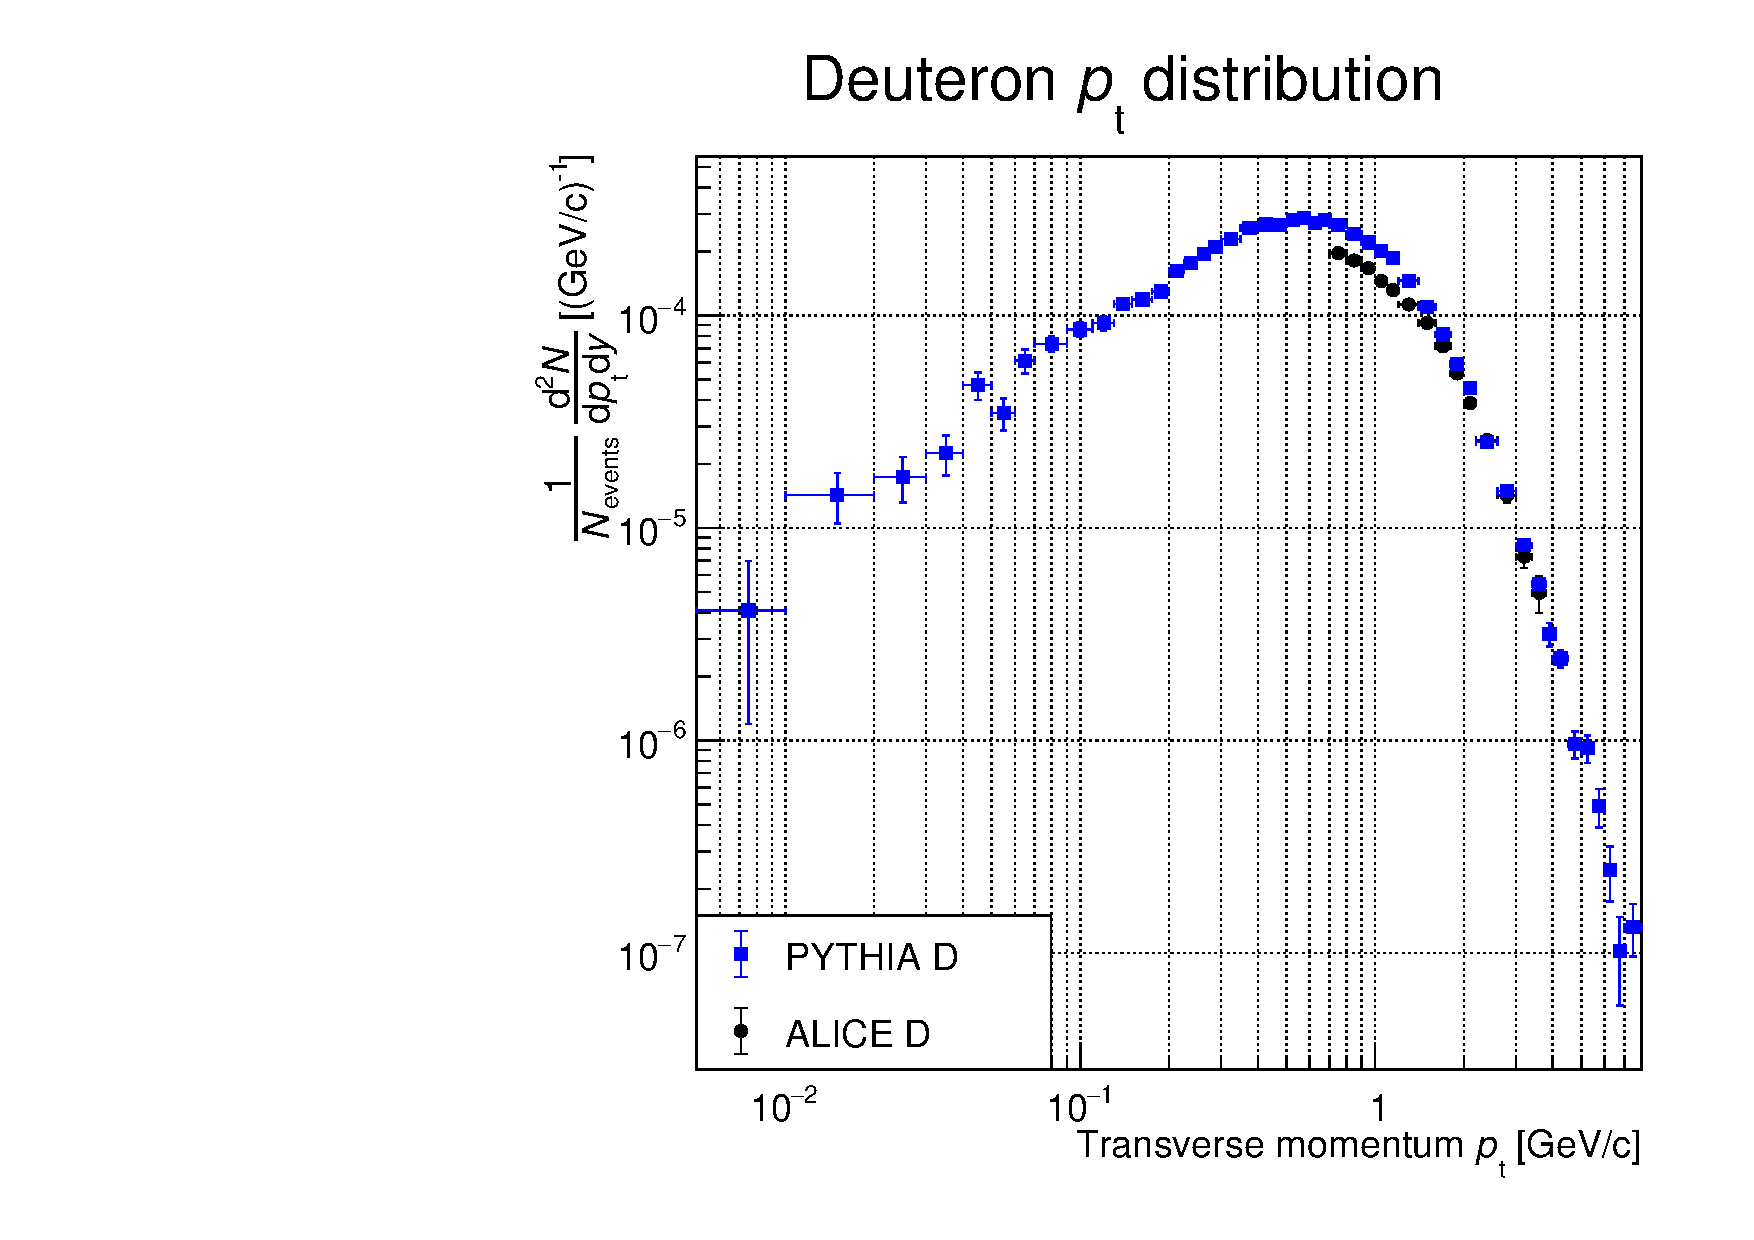
\includegraphics[width=\textwidth]{image/3-risultati/analyse/A/deuteron.pdf}
        \caption{}
        \label{fig:A_deuteron}
    \end{subfigure}
    %\hspace{1cm}
    \begin{subfigure}{.49\textwidth}
        \centering
        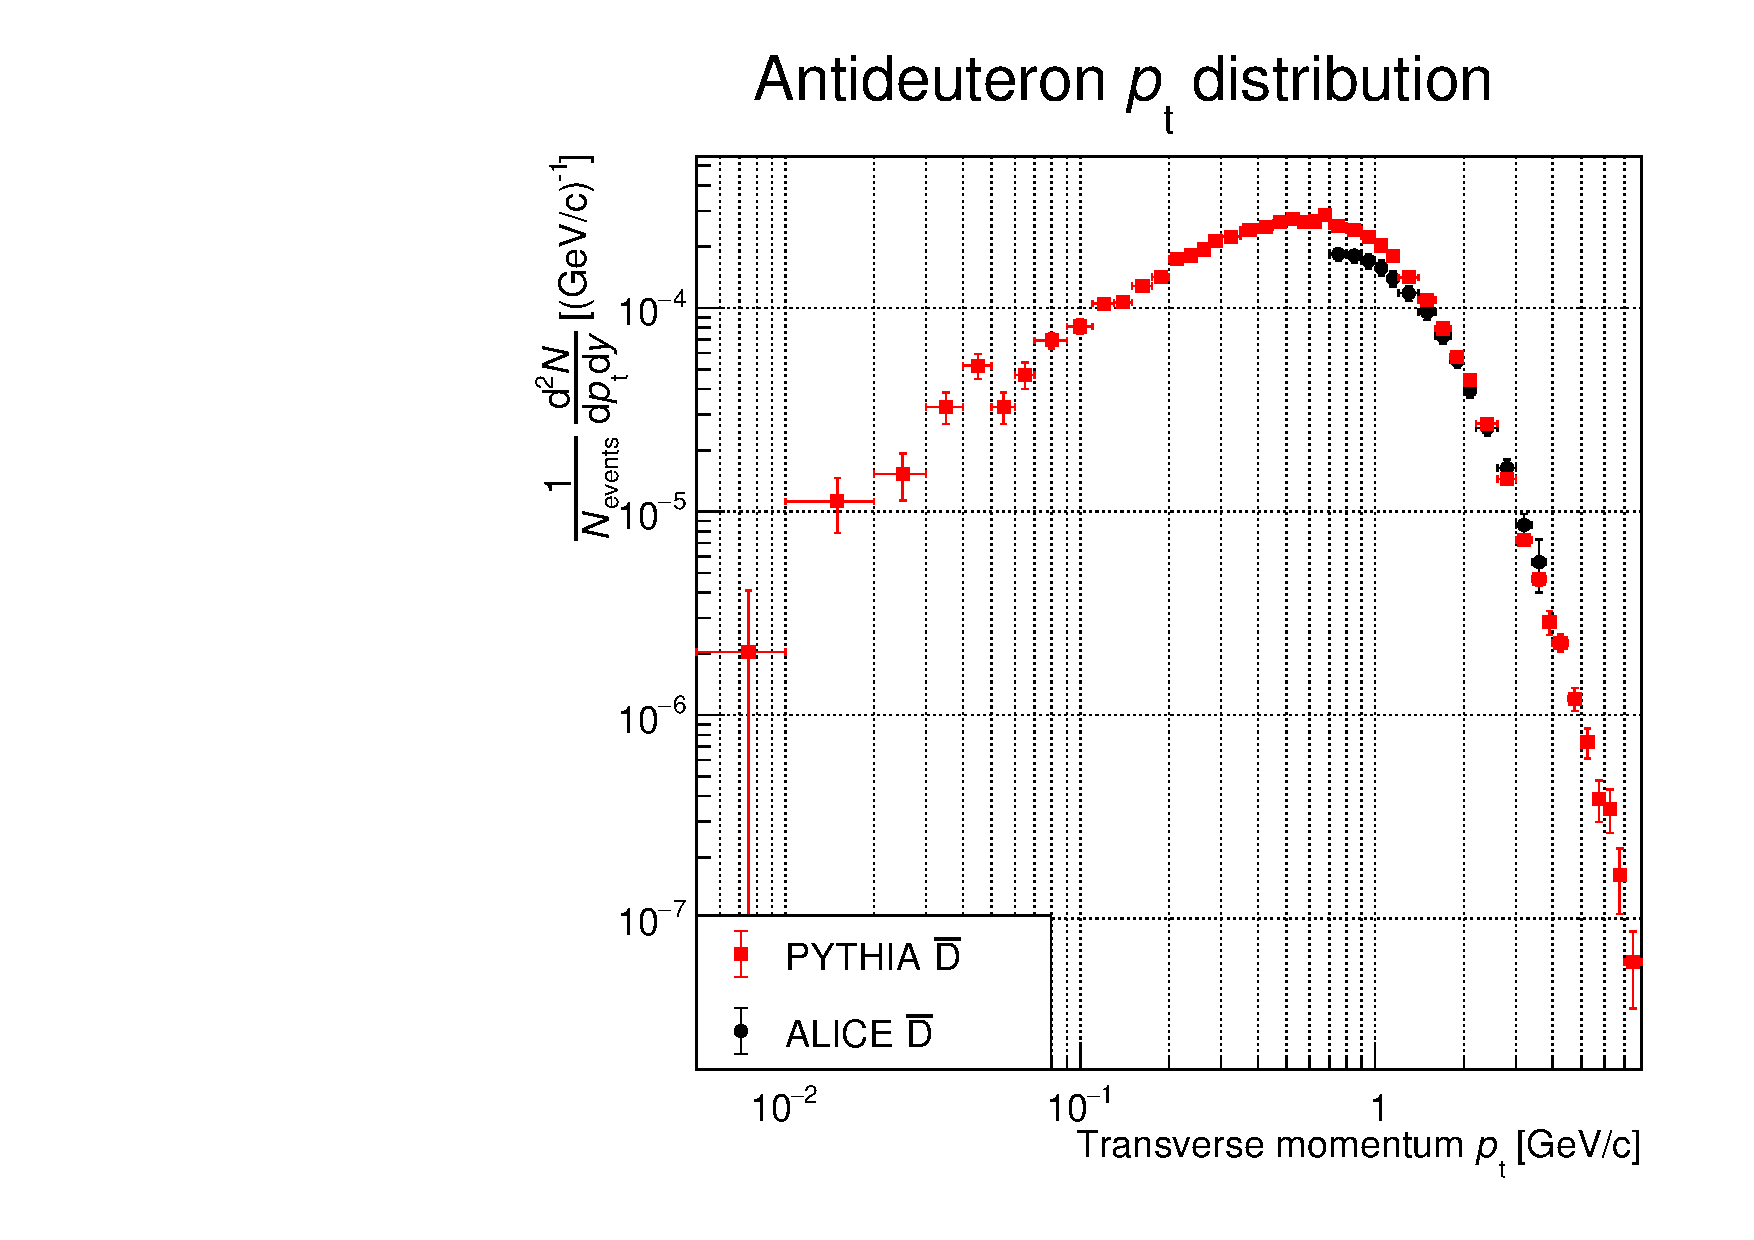
\includegraphics[width=\textwidth]{image/3-risultati/analyse/A/antideuteron.pdf}
        \caption{}
        \label{fig:A_antideuteron}
    \end{subfigure}
    \captionwithsource{Distribuzione dell'impulso trasverso di \emph{\rmfamily (a)} $D$ e \emph{\rmfamily (b)} di $\bar D$ in confronto con i dati di ALICE.}{\cite{ALICE:2020foi}}
    \label{fig:A_(anti)deuteron}
\end{figure}

In \autoref{fig:A_pp} osserviamo lo spettro di produzione della somma di protoni e antiprotoni nel caso in cui la produzione deuteronica sia attivata e non attivata, messo in confronto con i dati sperimentali.
Da questo grafico possiamo dedurre che la riproduzione di \pythiaa{} dello spettro dei protoni è fedele solamente nell'intorno di $p_t \sim 1$ GeV/$c$.
Gli andamenti degli spettri con produzione attivata e disattivata non presentano  particolari differenze, se non negli impulsi più alti, ma ciò è dovuto alle maggiori fluttuazioni dovute alla minore statistica.
Eseguendo un rapporto dei due istogrammi, visibile in \autoref{fig:A_ratio_pp_ON_OFF}, si ottiene che la media pesata del valore della frazione risulta essere $0.9988 \pm 0.0002$, inferiore a 1, compatibile con il valore atteso di 0.999.
Bisogna menzionare che le predizioni per la produzione di protoni da \pythiaa{} sono note per non descrivere fedelmente le misure sperimentali.
Questo è perché il tune di \pythiaa{} non è stato ottimizzato per riprodurre la produzione di nucleoni all'LHC, ma è comunque utilizzato come base per la maggior parte delle predizioni ed è stato utilizzato per la stima dei parametri per la sezione d'urto efficace, giustificando la scelta del \textit{tuning} per questo studio.
La produzione dei (anti)nuclei dipende essa stessa dallo spettro di produzione di protoni, che risulta interconnessa con tali parametri, ma la descrizione delle misure di protoni esula dallo scopo di questa tesi.

Se andiamo a confrontare invece lo spettro dei deuteroni e degli antideuteroni con i dati di ALICE \cite{ALICE:2020foi}, osserviamo in \autoref{fig:A_(anti)deuteron} che la produzione (anti)deuteronica è accurata solamente per gli impulsi più alti, nell'intorno di $p_t \sim 3$ GeV/$c$.
Infatti, eseguendo una divisione tra i dati di \pythia e di ALICE per i (anti)deuteroni, è possibile osservare che il rapporto si avvicina al valore unitario in quell'intorno, come si vede in \autoref{fig:A_division}.
In generale si osserva una sovrapproduzione sia per i deuteroni e sia per gli antideuteroni, con le medie pesate rispettivamente di $1.203 \pm 0.017$ e di $1.129 \pm 0.023$.
\begin{figure}[htb]
    \centering
    \begin{subfigure}{.49\textwidth}
    \centering
        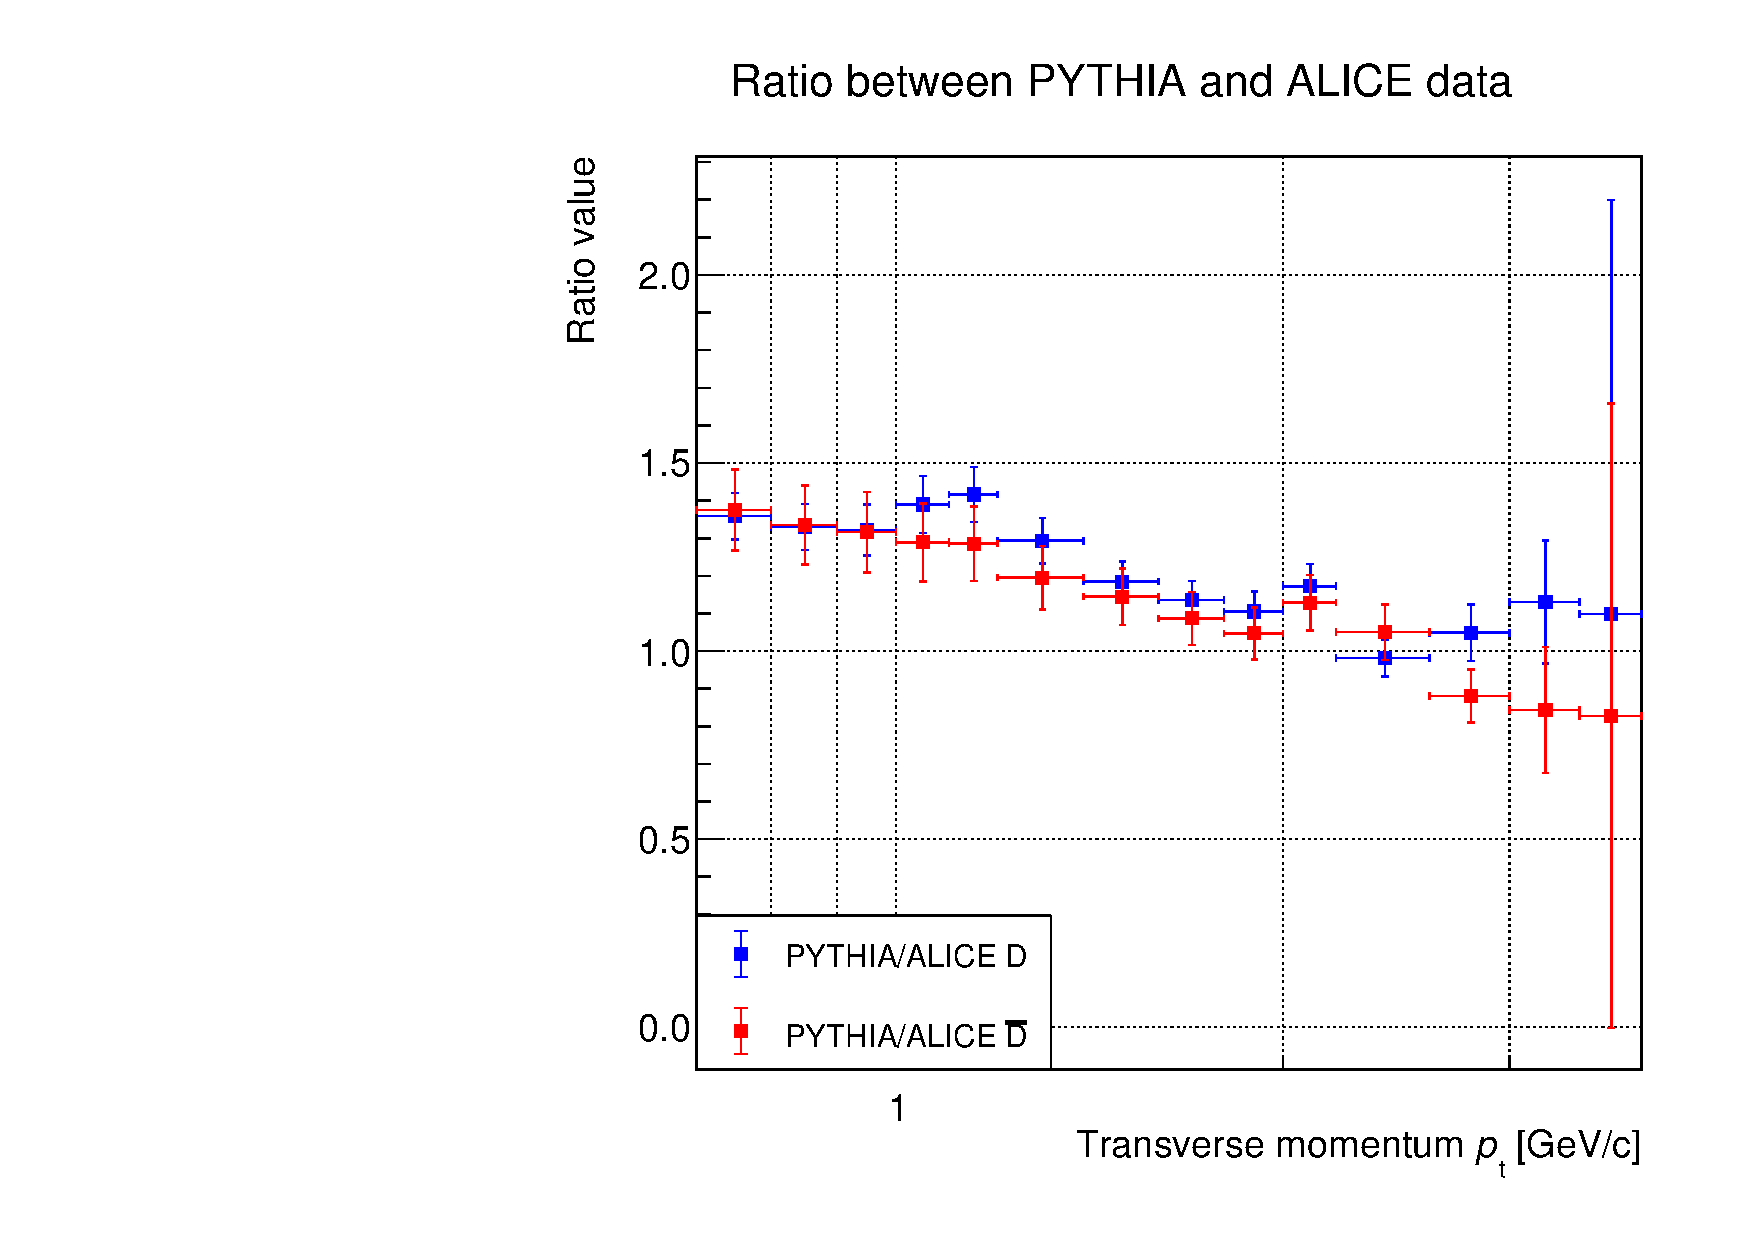
\includegraphics[width=\textwidth]{image/3-risultati/analyse/A/division.pdf}
        \caption{}
        \label{fig:A_division}
    \end{subfigure}
    %\hspace{1cm}
    \begin{subfigure}{.49\textwidth}
        \centering
        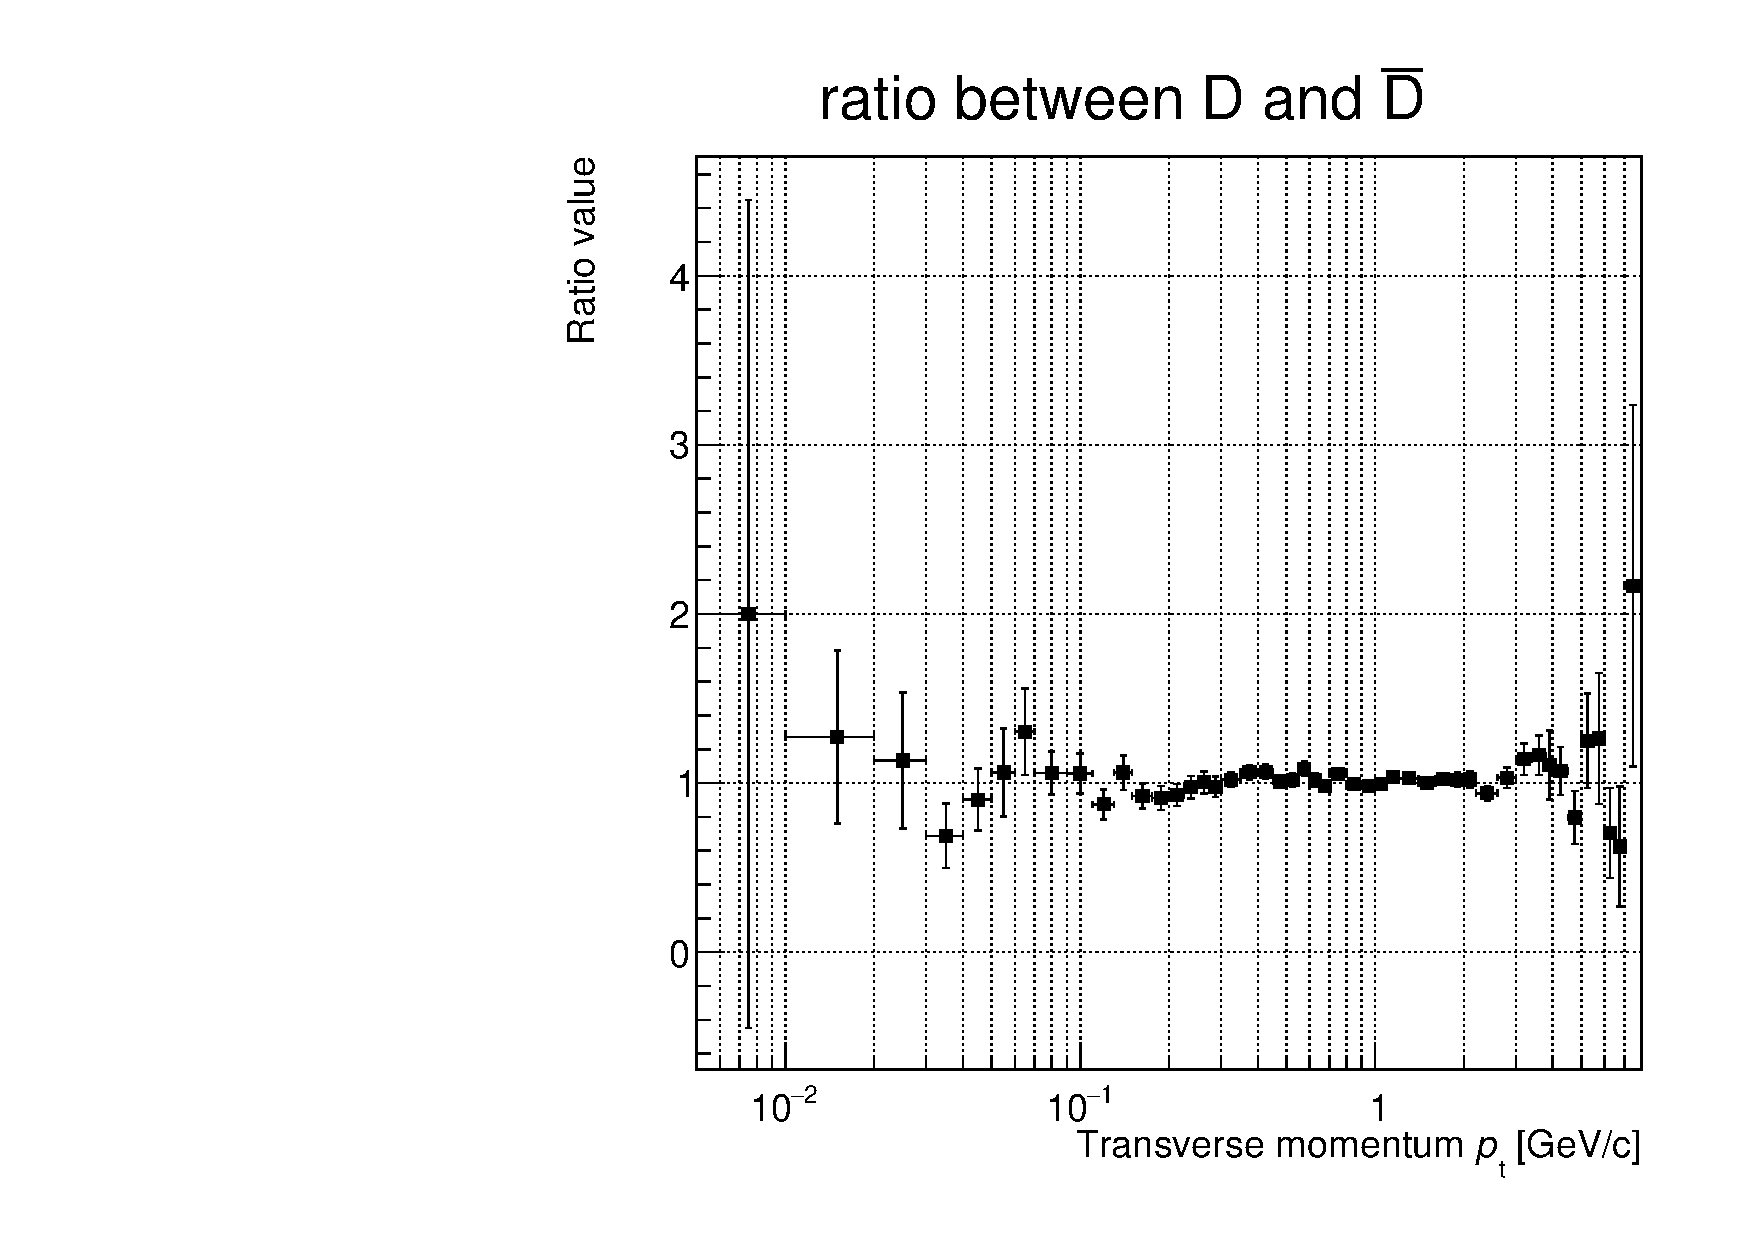
\includegraphics[width=\textwidth]{image/3-risultati/analyse/A/ratio_DD.pdf}
        \caption{}
        \label{fig:A_ratio_DD}
    \end{subfigure}
    \caption{\emph{\rmfamily (a)} Divisione tra la distribuzione dell'impulso trasverso di $D$ e $\bar D$ con i dati di ALICE. \emph{\rmfamily (b)} Rapporto delle distribuzione dell'impulso trasverso di $D$ con quello di $\bar D$.}
    \label{fig:A_ratio_DD_}
\end{figure}

Per verificare ulteriormente la correttezza delle predizioni si è fatto un ulteriore rapporto, riportato in \autoref{fig:A_ratio_DD}, tra lo spettro dei deuteroni e lo spettro degli antideuteroni.
La media pesata del rapporto risulta essere $1.013 \pm 0.008$, con una leggera sovrapproduzione di deuteroni.
%%%%%%%%%%%%%%%%%%%%%%%%%%%%%%%%%%%%%%%%%%
\section{I principali canali di produzione}\label{ch:channels}
Andando ad analizzare invece quali siano i canali che producono più deuteroni, si è andati \textit{in primis} a riempire gli istogrammi relativi alle particelle di partenza, ossia si è andato a vedere per ogni deuterone prodotto quali siano le loro particelle madri.
Per semplificare la nomenclatura, prendendo in considerazione la \autoref{tab:canali}, chiameremo i canali (1-4) "canali $pn$", i canali (5-6) "canali $pp$" e i canali (7-8) "canali $nn$".
Lo stesso vale per gli antideuteroni con canali $\bar p\bar n$, $\bar p\bar p$ e $\bar n\bar n$.
Da ciò abbiamo tre distribuzioni per i deuteroni e tre per gli antideuteroni, rispettivamente con i canali $pn$, $pp$, $nn$ e $\bar p\bar n$, $\bar p\bar p$, $\bar n\bar n$.
In \autoref{fig:A_ov_deut} e in \autoref{fig:A_ov_antideut} vengono riportate le distribuzioni di questi canali in sovrapposizione, mentre in \autoref{fig:A_ov_stack_deut} e in \autoref{fig:A_ov_stack_antideut} viene riportata la produzione relativa di (anti)deuteroni.  
Si può osservare che \pythiaa{} assegna a ognuno di questi canali uno stesso peso nella produzione sia deuteronica e sia antideuteronica, se non per un piccolo incremento per il canale $pn$ nei deuteroni e il canale $\bar p\bar n$ negli antideuteroni.\\

Successivamente si è andati ad analizzare la produzione relativa dei subcanali dei canali $pn$, $pp$ e $nn$ e delle relative antiparticelle, andando a vedere quali siano i loro principali contributi.
In \autoref{fig:A_deut_subchannels} e in \autoref{fig:A_antideut_subchannels} possiamo osservare tali contributi.
Si nota che il contributo più abbondante per tutti e sei i canali è quello in cui avviene la produzione di un (anti)deuterone e di un pione, mentre il contributo minore nella produzione è la cattura radiativa.
Invece la produzione di un deuterone e di due pioni è meno abbondante, perché essa richiede più energia ed è meno probabile che avvenga.

È curioso notare che in \autoref{fig:A_pn_stack_deut} e in \autoref{fig:A_pn_stack_antideut} il processo $pn\to \pi^+\pi^- D$ ($ \bar p \bar n\to \pi^+\pi^- \bar D$) pare più abbondante del processo $pn\to \pi^0\pi^0D$ ($ \bar p \bar n\to \pi^0\pi^0 \bar D$).
Questo può essere spiegato con l'invarianza di isospin, per cui si ha che (\cite{Dal_2015})
\begin{equation}
    \sigma_{pn\to\pi^+\pi^-D} = 2\sigma_{pn\to\pi^0\pi^0D} + \dfrac12\sigma_{pp\to\pi^+\pi^0D}
\end{equation}
con $\sigma_\text{processo}$ la sezione d'urto del processo associato.
\begin{figure}[htbp]
    \centering
    \begin{subfigure}{.49\textwidth}
    \centering
        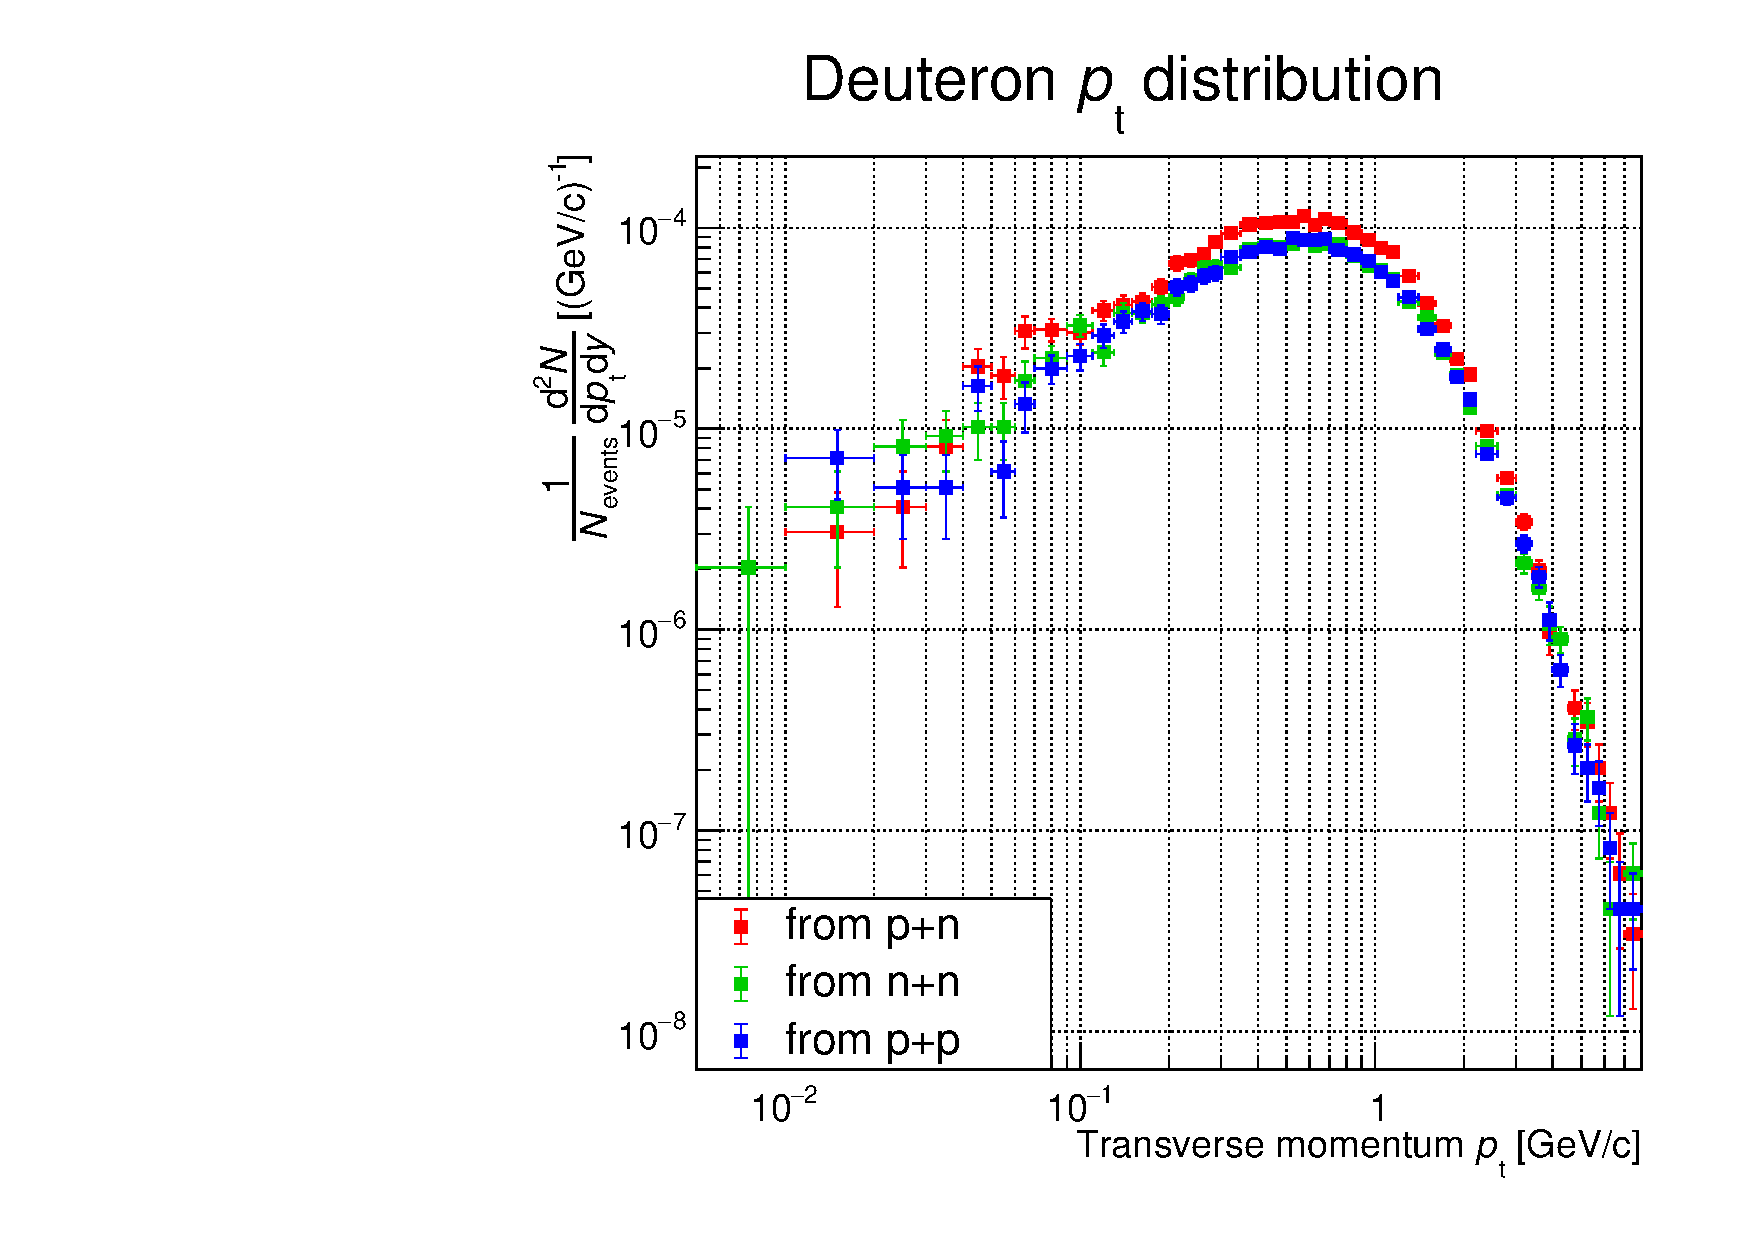
\includegraphics[width=\textwidth]{image/3-risultati/deuteron_analyse/A/ov_log.pdf}
        \caption{}
        \label{fig:A_ov_deut}
    \end{subfigure}
    %\hspace{1cm}
    \begin{subfigure}{.49\textwidth}
        \centering
        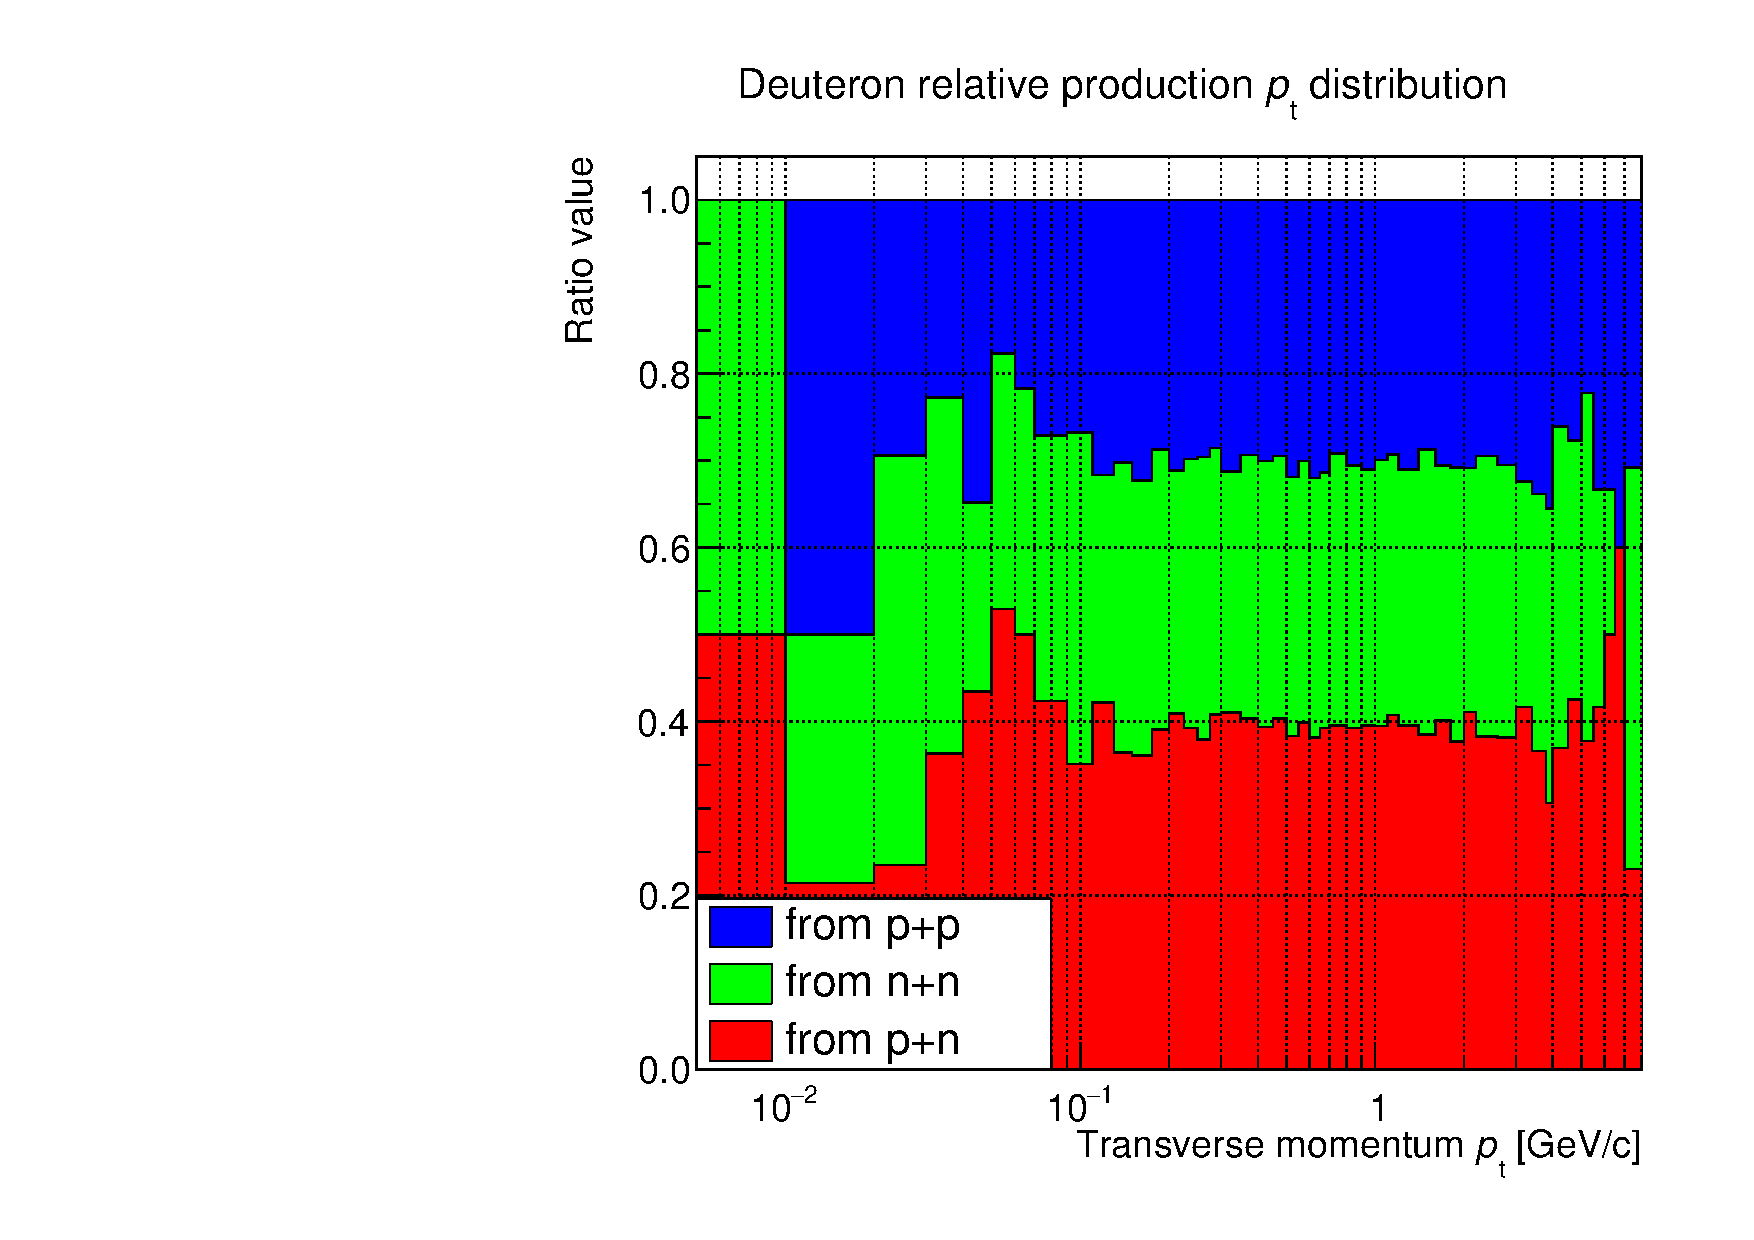
\includegraphics[width=\textwidth]{image/3-risultati/deuteron_analyse/A/ov_stack.pdf}
        \caption{}
        \label{fig:A_ov_stack_deut}
    \end{subfigure}
    \begin{subfigure}{.49\textwidth}
    \centering
        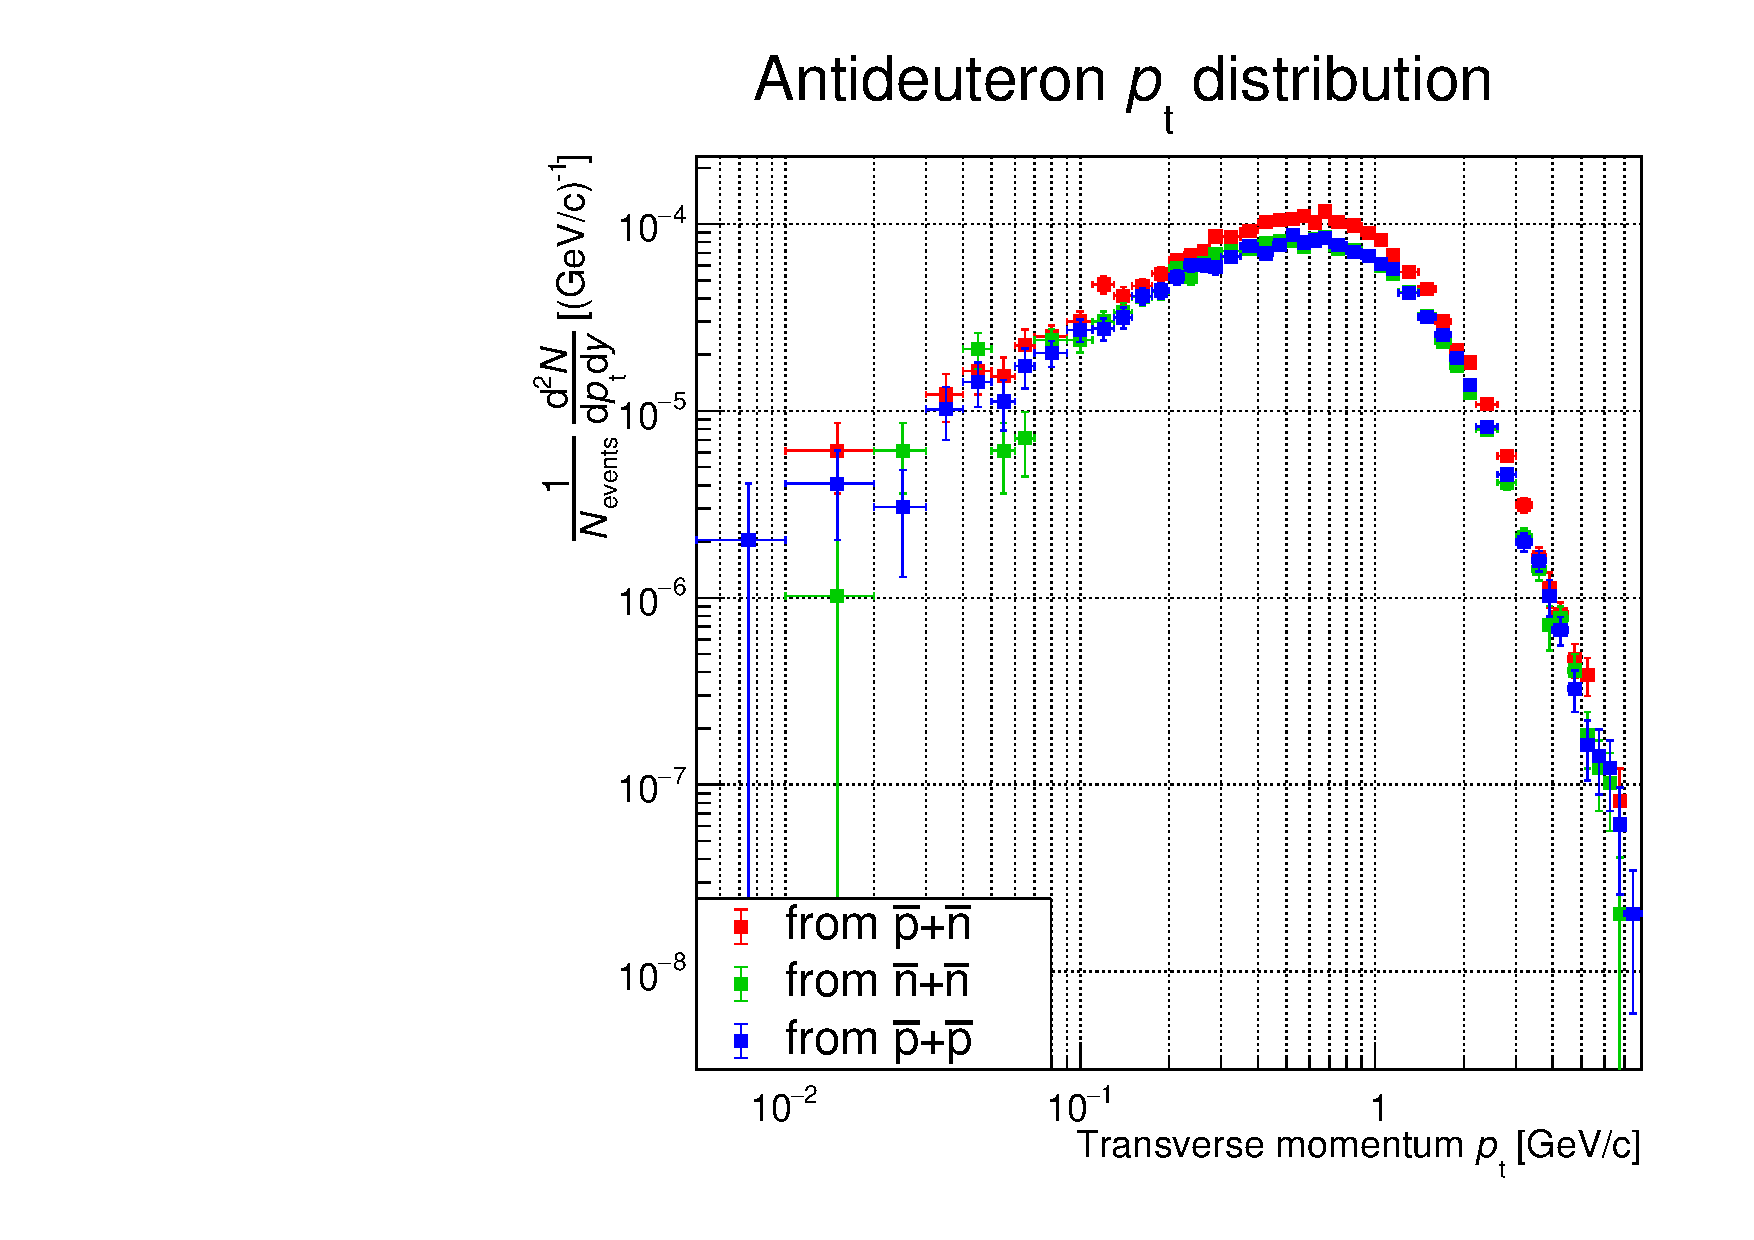
\includegraphics[width=\textwidth]{image/3-risultati/antideuteron_analyse/A/ov_log.pdf}
        \caption{}
        \label{fig:A_ov_antideut}
    \end{subfigure}
    %\hspace{1cm}
    \begin{subfigure}{.49\textwidth}
        \centering
        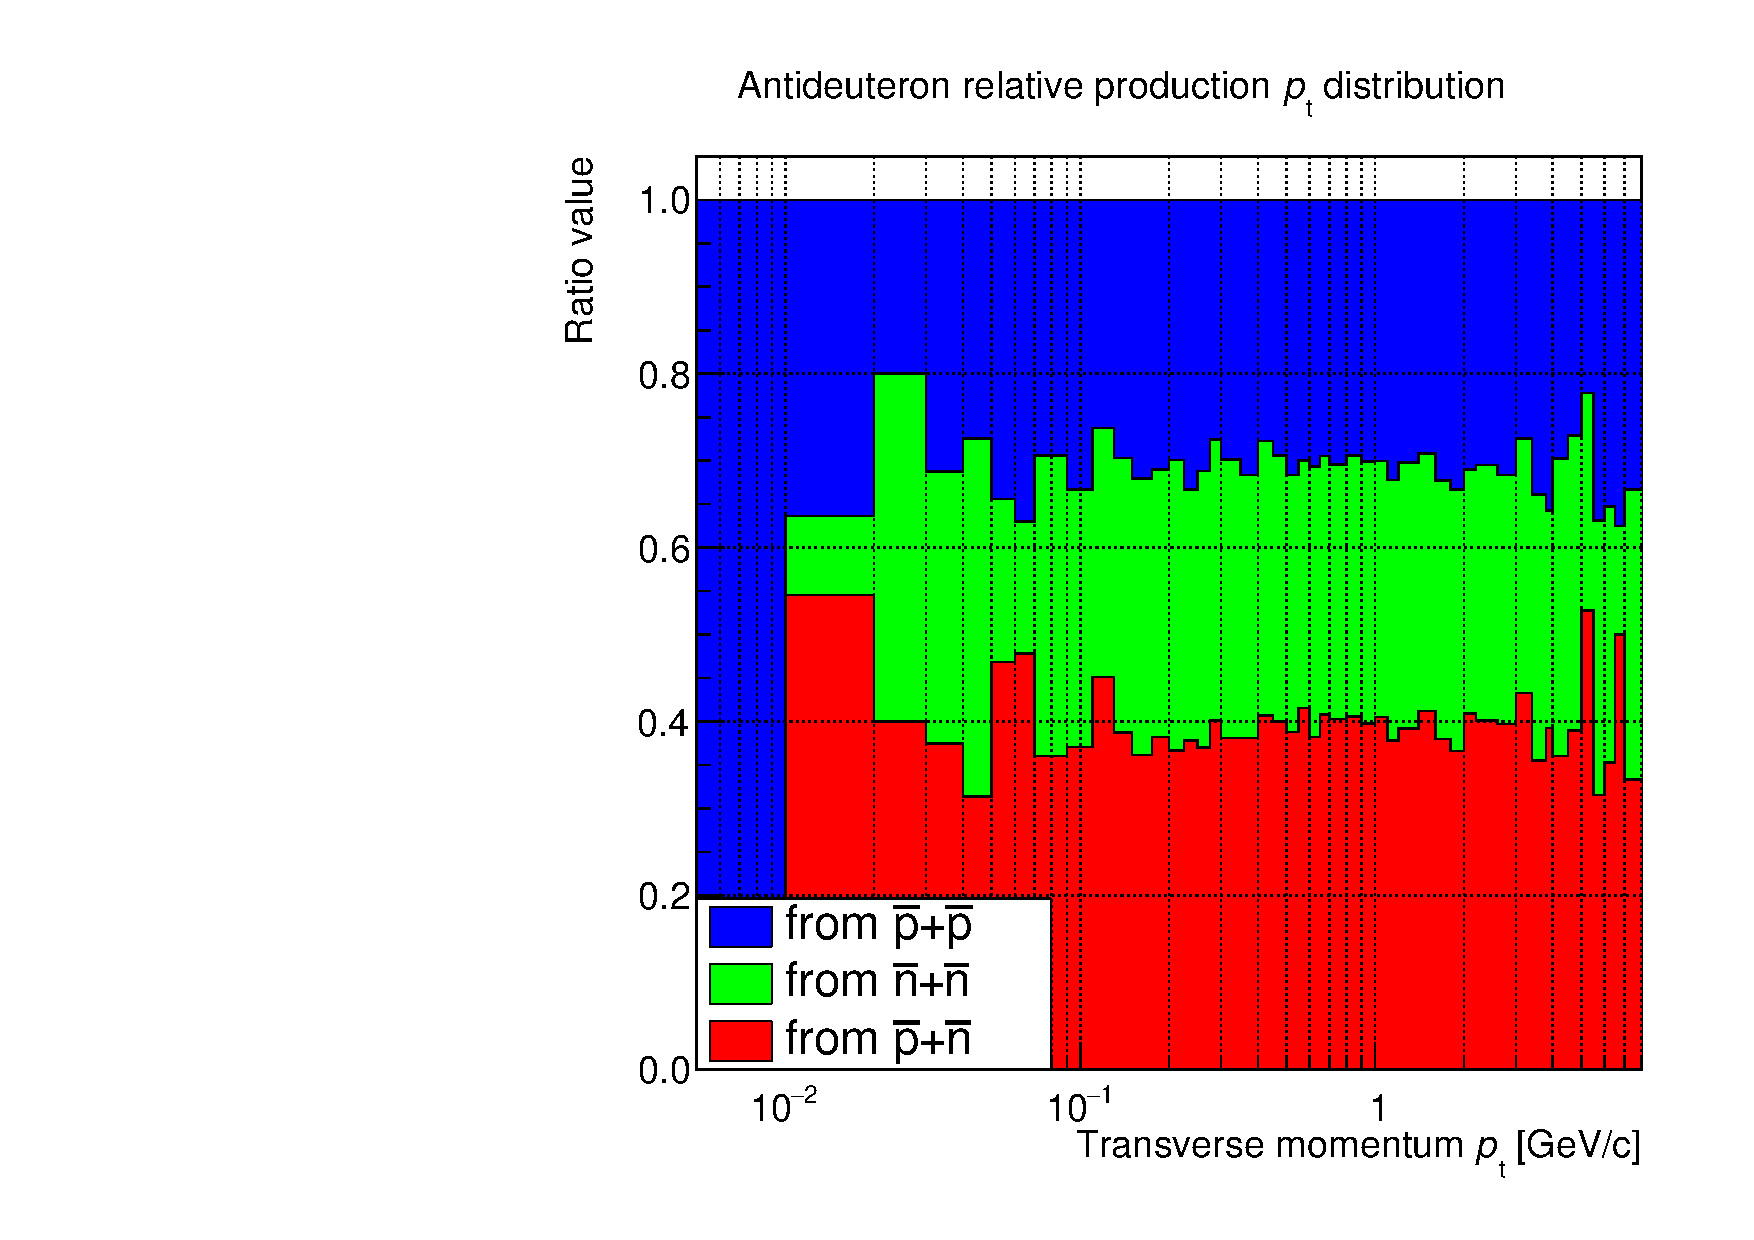
\includegraphics[width=\textwidth]{image/3-risultati/antideuteron_analyse/A/ov_stack.pdf}
        \caption{}
        \label{fig:A_ov_stack_antideut}
    \end{subfigure}
    \caption{\emph{\rmfamily (a)} Distribuzioni dell'impulso trasverso di $D$ dei canali $pn$, $pp$ e $nn$ e \emph{\rmfamily (b)} la produzione relativa nei vari canali di $D$. \emph{\rmfamily (c)} Distribuzioni dell'impulso trasverso di $\bar D$ dei canali $\bar p\bar n$, $\bar p\bar p$ e $\bar n\bar n$ e \emph{\rmfamily (d)} la produzione relativa nei vari canali di $\bar D$.}
    \label{fig:A_ov}
\end{figure}
\begin{figure}[htbp]
    \centering
    \begin{subfigure}{.49\textwidth}
    \centering
        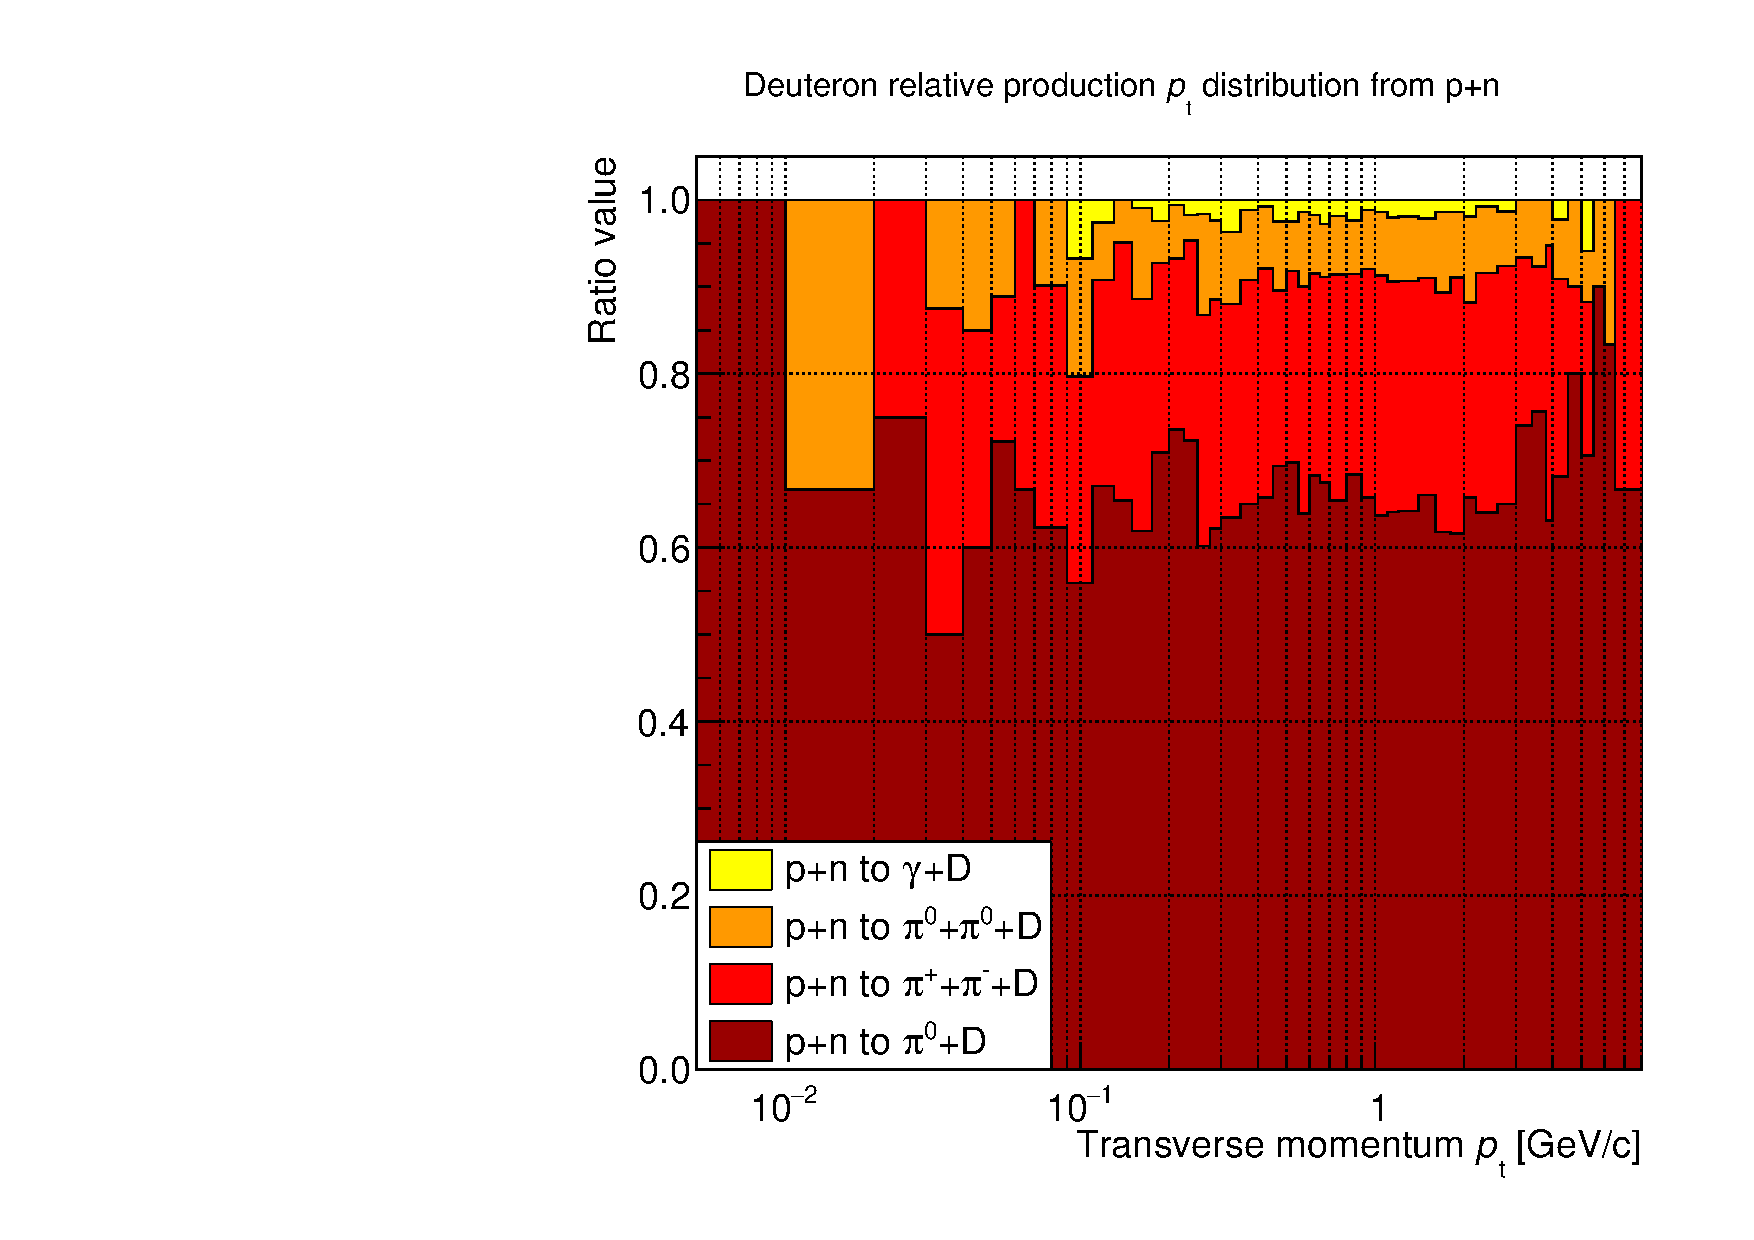
\includegraphics[width=\textwidth]{image/3-risultati/deuteron_analyse/A/p_n_stack.pdf}
        \caption{}
        \label{fig:A_pn_stack_deut}
    \end{subfigure}
    %\hspace{1cm}
    \begin{subfigure}{.49\textwidth}
        \centering
        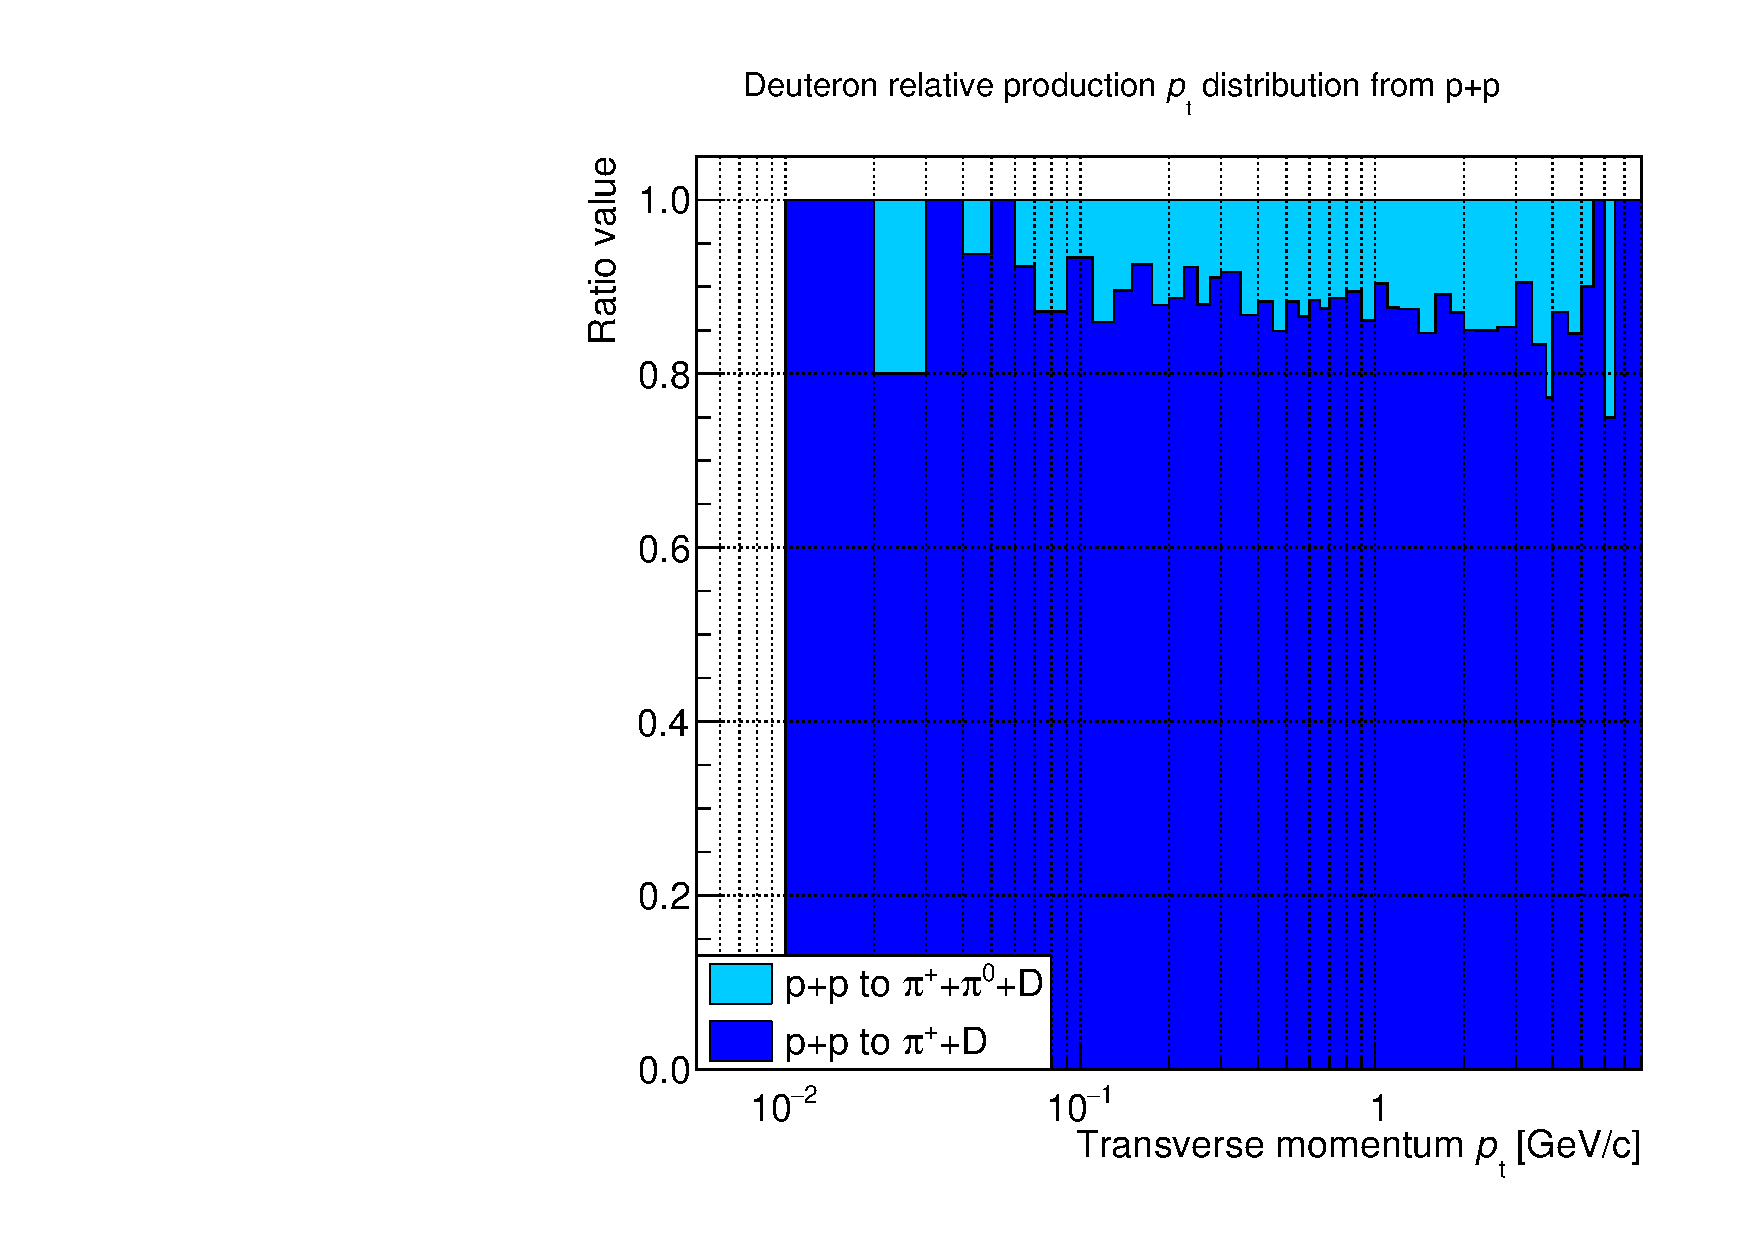
\includegraphics[width=\textwidth]{image/3-risultati/deuteron_analyse/A/p_p_stack.pdf}
        \caption{}
        \label{fig:A_pp_stack_deut}
    \end{subfigure}
    \begin{subfigure}{.49\textwidth}
    \centering
        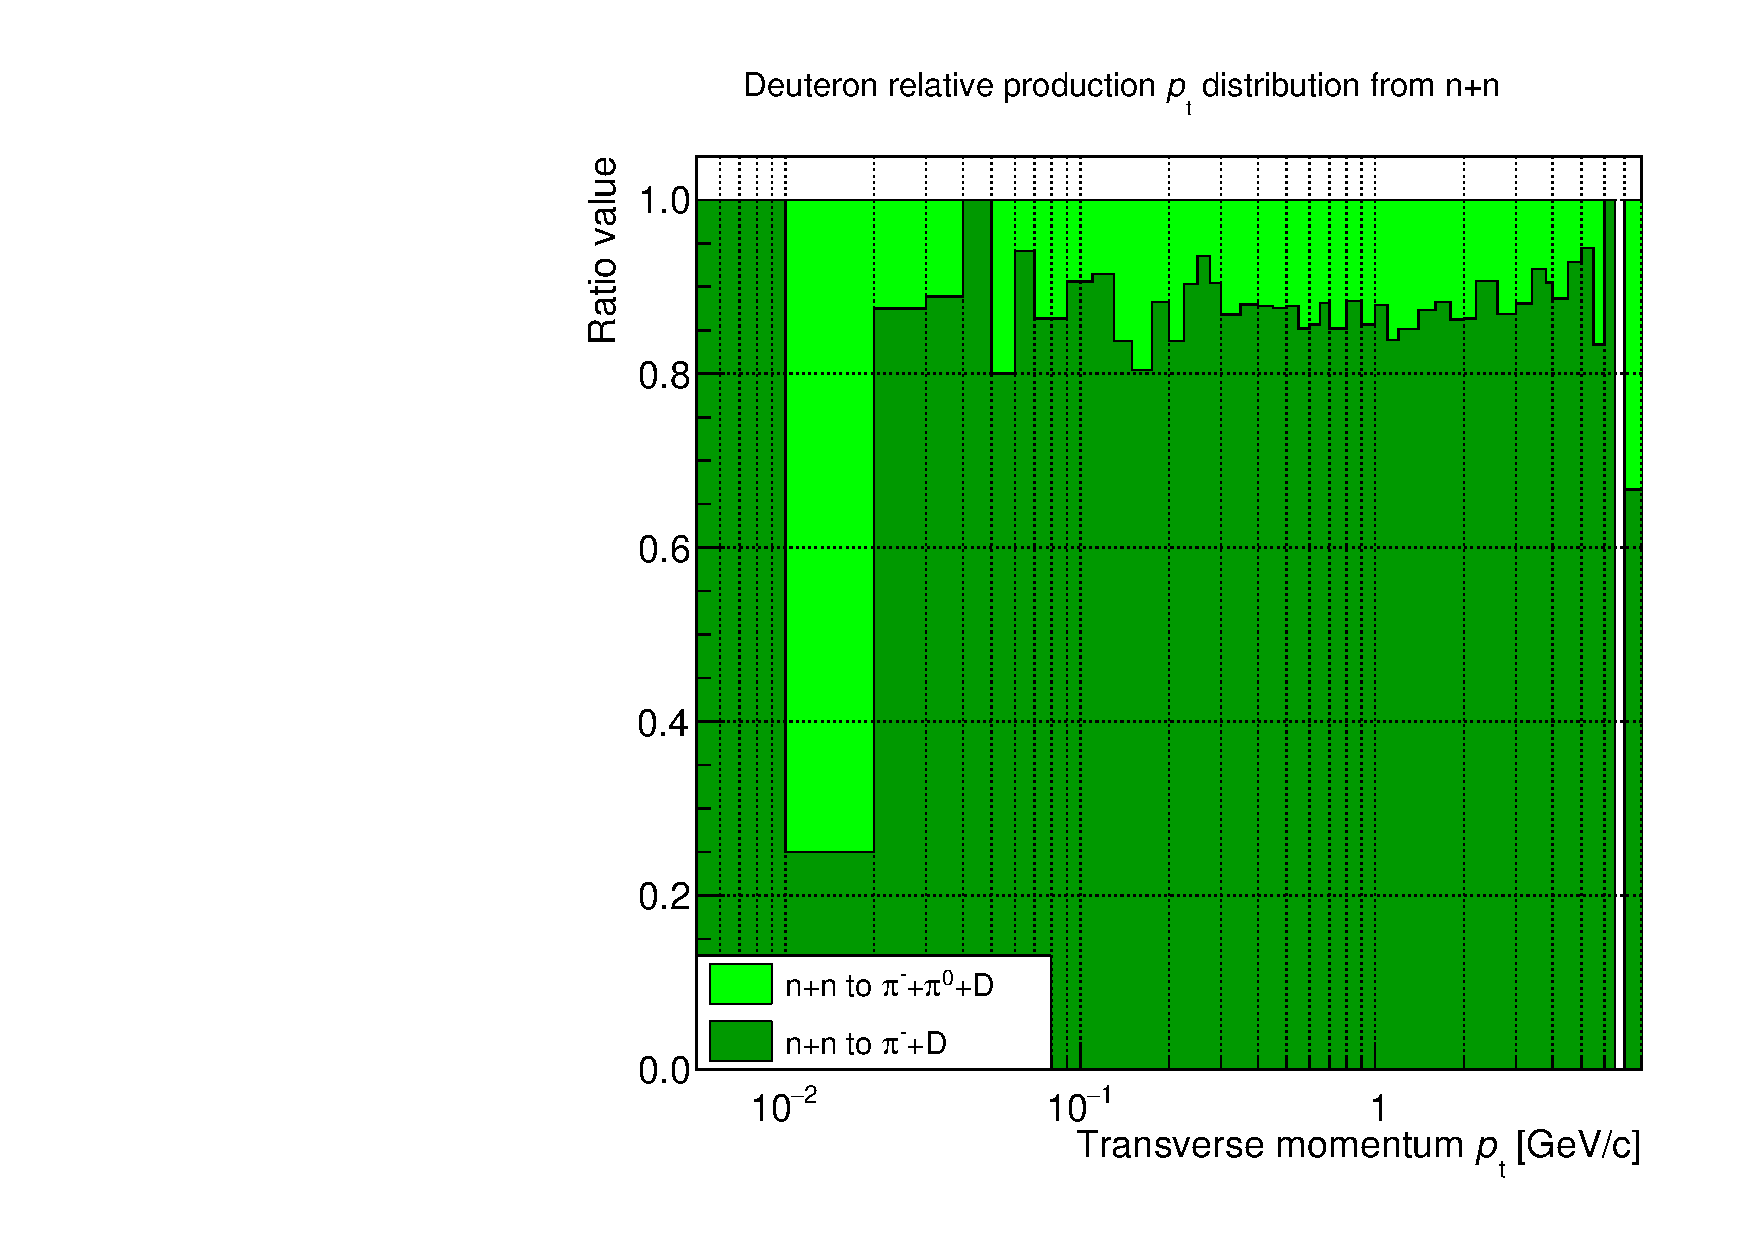
\includegraphics[width=\textwidth]{image/3-risultati/deuteron_analyse/A/n_n_stack.pdf}
        \caption{}
        \label{fig:A_nn_stack_deut}
    \end{subfigure}
    \caption{Produzione relativa di $D$ dei canali \emph{\rmfamily (a)} $pn$, \emph{\rmfamily (b)} $pp$ e \emph{\rmfamily (c)} $nn$.}
    \label{fig:A_deut_subchannels}
\end{figure}
\begin{figure}[htbp]
    \centering
    \begin{subfigure}{.49\textwidth}
    \centering
        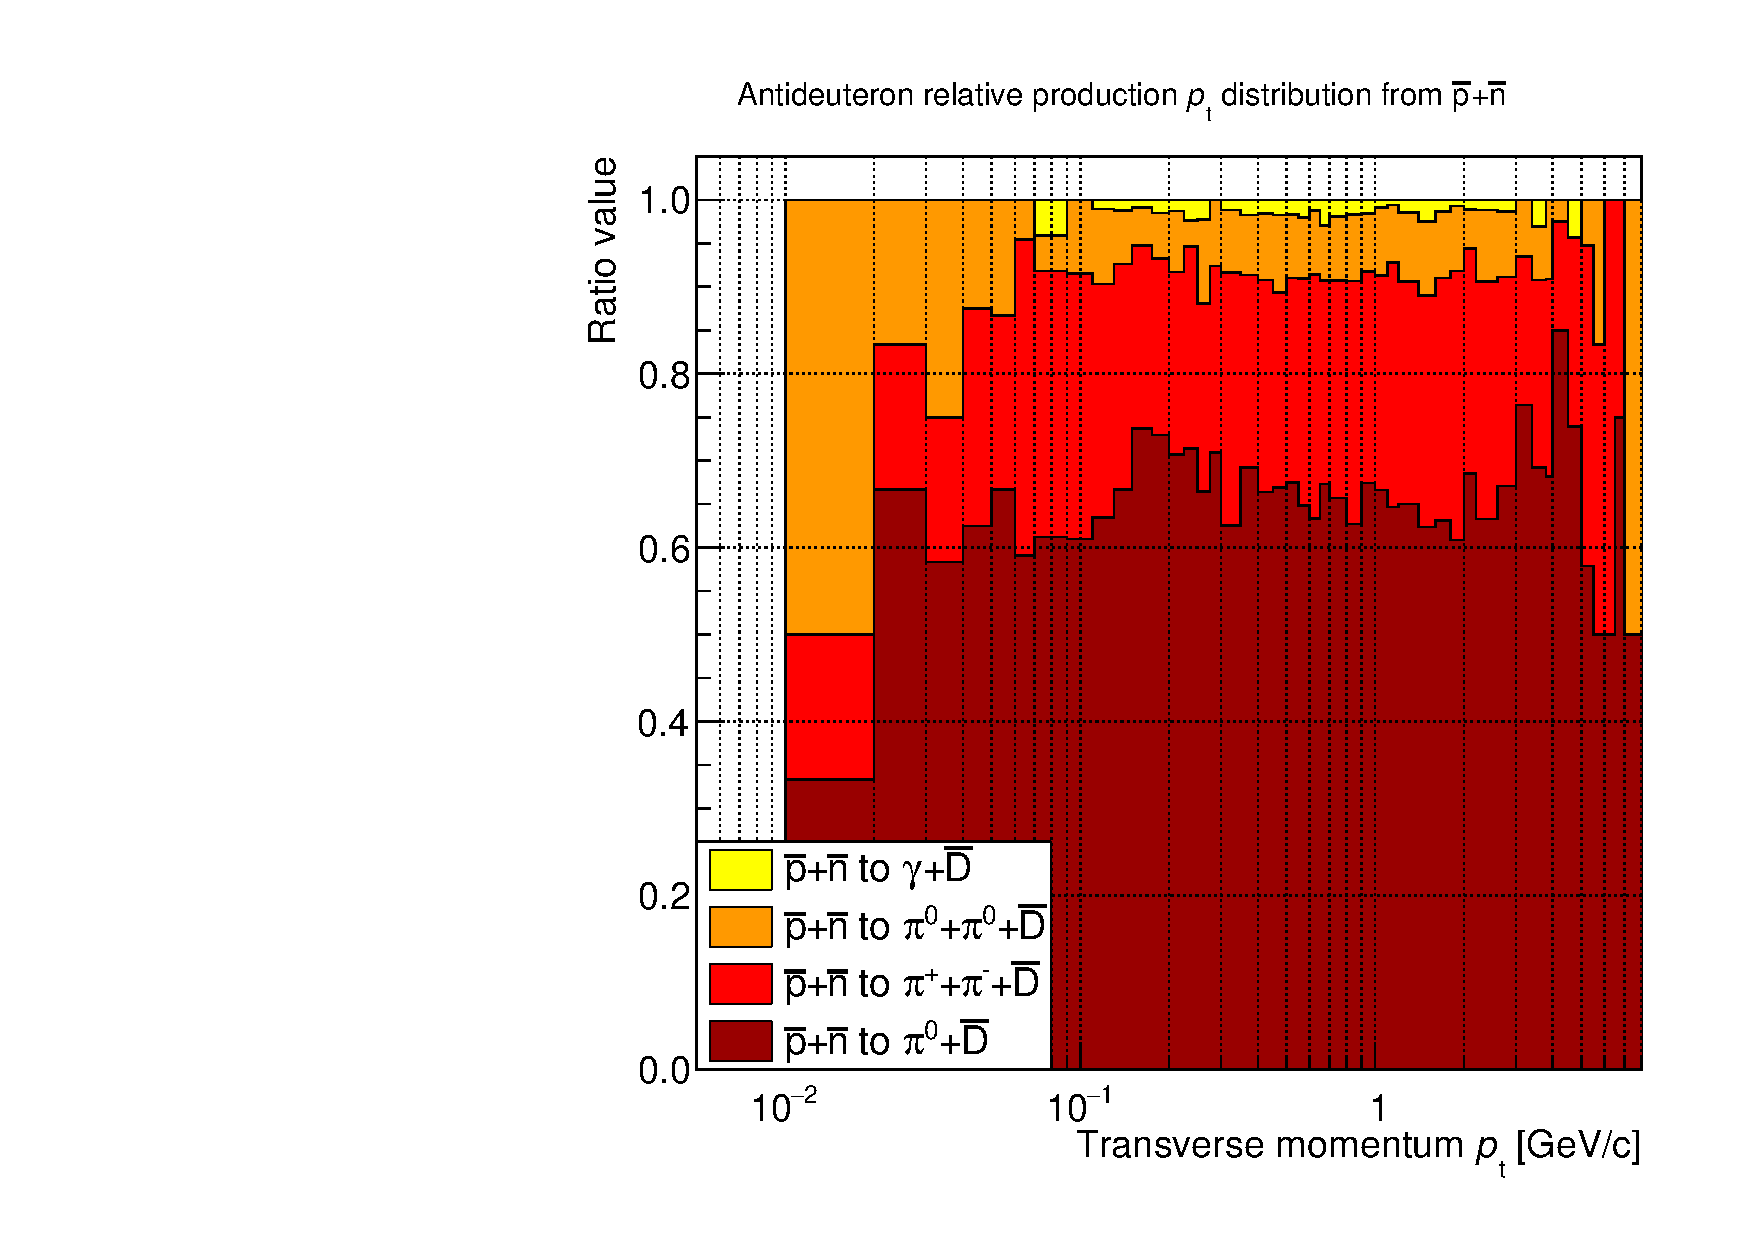
\includegraphics[width=\textwidth]{image/3-risultati/antideuteron_analyse/A/p_n_stack.pdf}
        \caption{}
        \label{fig:A_pn_stack_antideut}
    \end{subfigure}
    %\hspace{1cm}
    \begin{subfigure}{.49\textwidth}
        \centering
        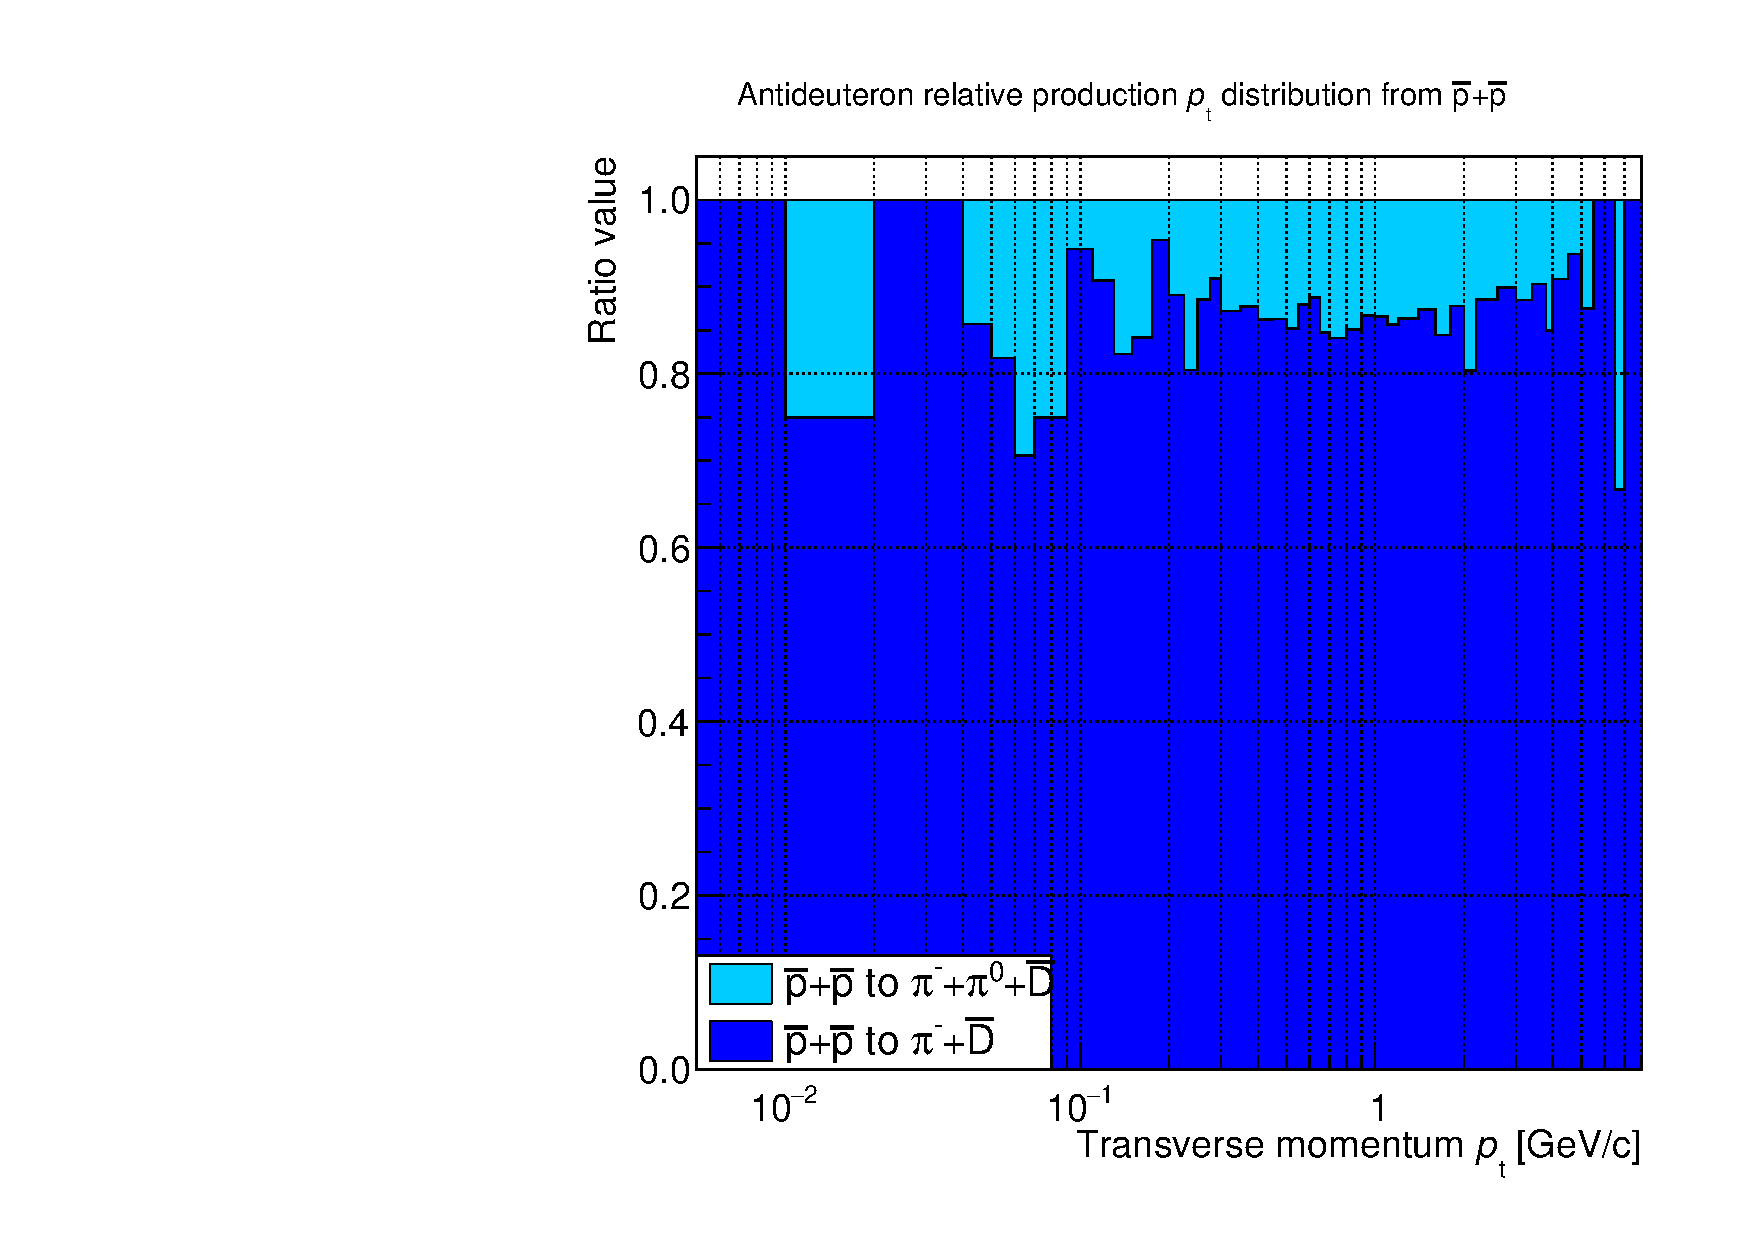
\includegraphics[width=\textwidth]{image/3-risultati/antideuteron_analyse/A/p_p_stack.pdf}
        \caption{}
        \label{fig:A_pp_stack_antideut}
    \end{subfigure}
    \begin{subfigure}{.49\textwidth}
    \centering
        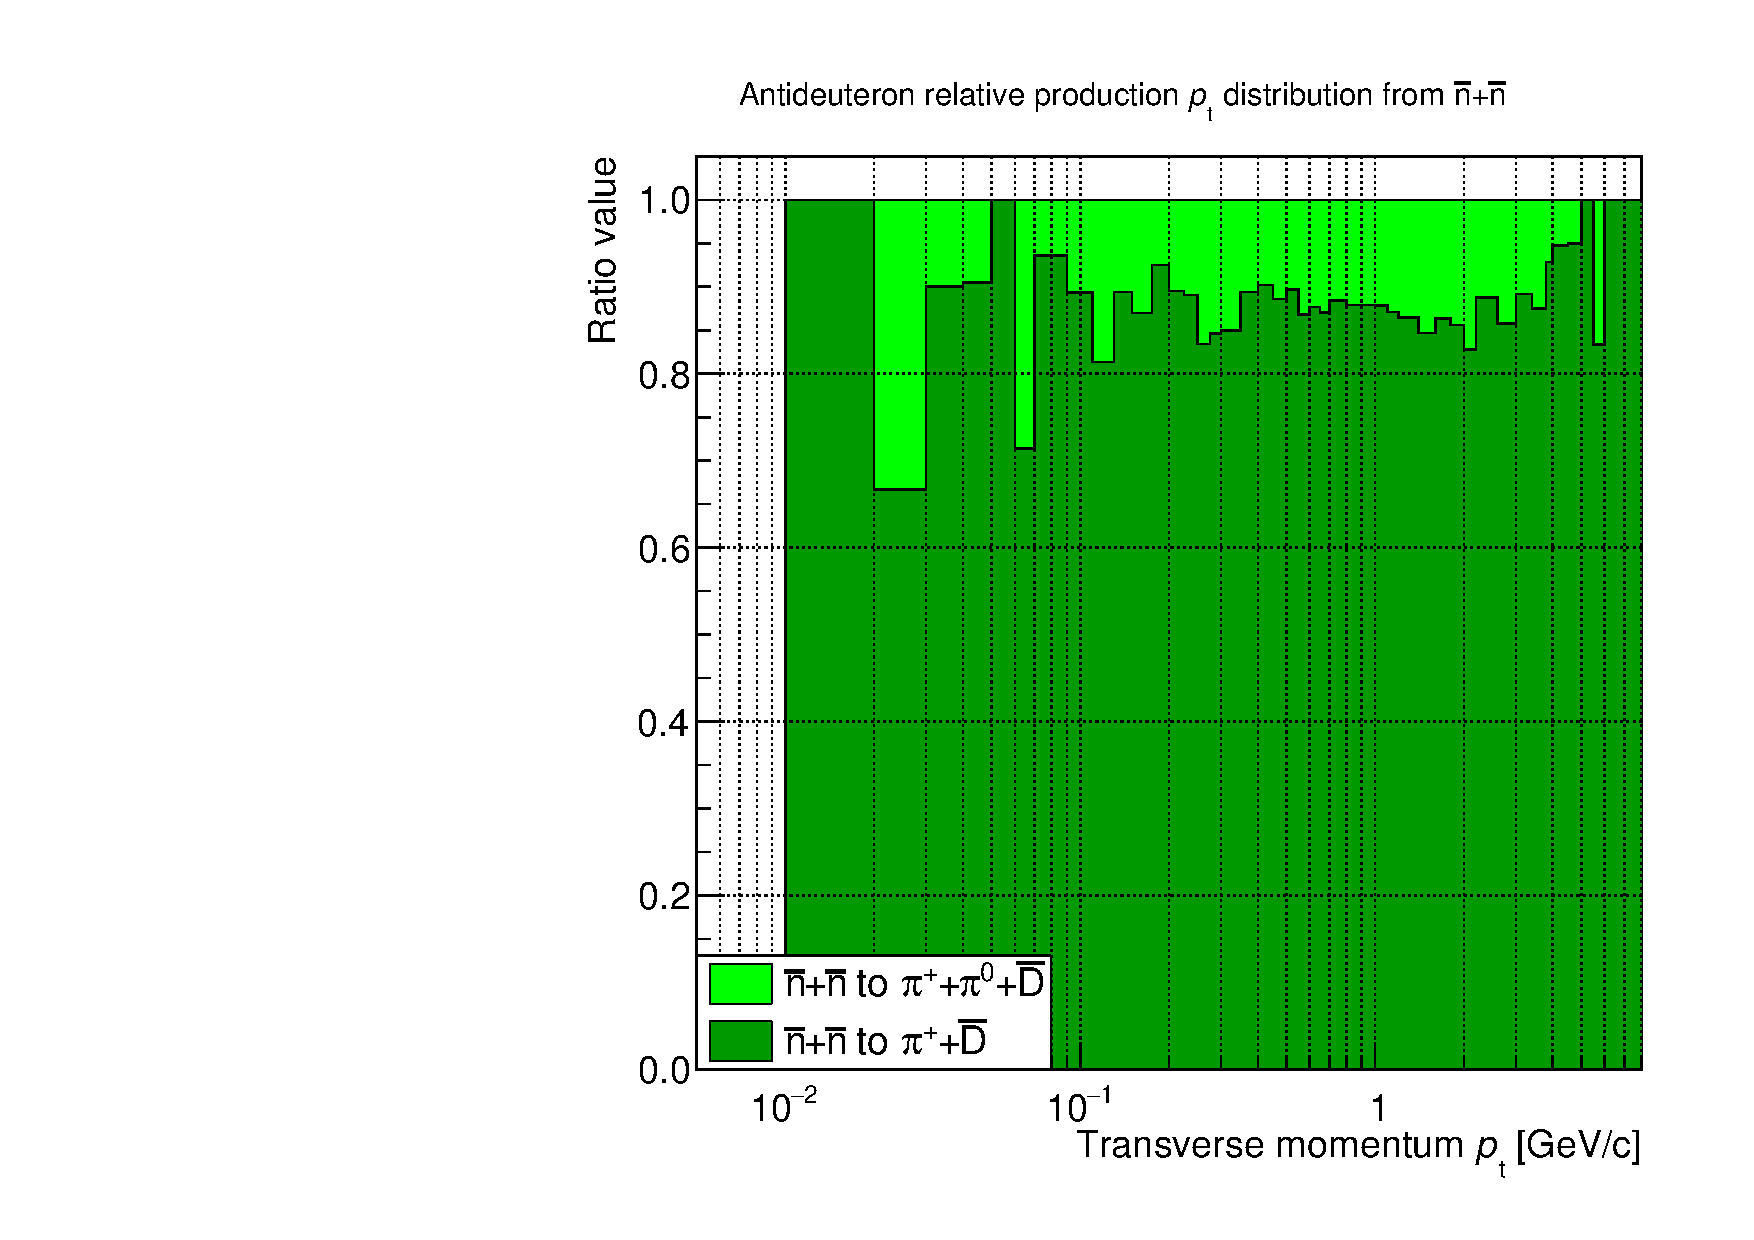
\includegraphics[width=\textwidth]{image/3-risultati/antideuteron_analyse/A/n_n_stack.pdf}
        \caption{}
        \label{fig:A_nn_stack_antideut}
    \end{subfigure}
    \caption{Produzione relativa di $\bar D$ dei canali \emph{\rmfamily (a)} $\bar p\bar n$, \emph{\rmfamily (b)} $\bar p\bar p$ e \emph{\rmfamily (c)} $\bar n\bar n$.}
    \label{fig:A_antideut_subchannels}
\end{figure}
%%%%%%%%%%%%%%%%%%%%%%%%%%%%%%%%%%%%%%%%%%%%%%%%%%%%
\section{Confronto del modello di coalescenza e di PYTHIA}
Sebbene non nella sua configurazione predefinita, \pythiaa{} ammette anche la produzione deuteronica tramite il modello di coalescenza.
Per far ciò si è andati a ridurre l'insieme di tutti i possibili canali di produzione al singolo canale della cattura radiativa (l'unico rilevante per la coalescenza), assegnando ad essa il modello di coalescenza con il parametro $p_0 = 195$ MeV.
La scelta di questo valore è giustificata da una semplice valutazione della \autoref{tab:valori_p0_1sigma0}: andando ad osservare la colonna $p_0$ si può dedurre che esso raggiunge stabilmente questo valore già a 7 TeV.
Dopodiché, oltre a questo, si è andati a imporre le condizioni già riportate nella \autoref{ch:settings} e si è effettuata la simulazione di Monte Carlo.\\

Andando a osservare lo spettro di produzione di $p+\bar p$ (visibile in \autoref{fig:E_pp}), non si nota una particolare differenza col modello predefinito, come deve essere, dal momento in cui il numero di (anti)deuteroni prodotti dovrebbe essere relativamente piccolo rispetto a quello dei protoni sia per il modello di \pythiaa{} sia per il modello di coalescenza.
\begin{figure}[htb]
    \centering
    \begin{subfigure}{.49\textwidth}
    \centering
        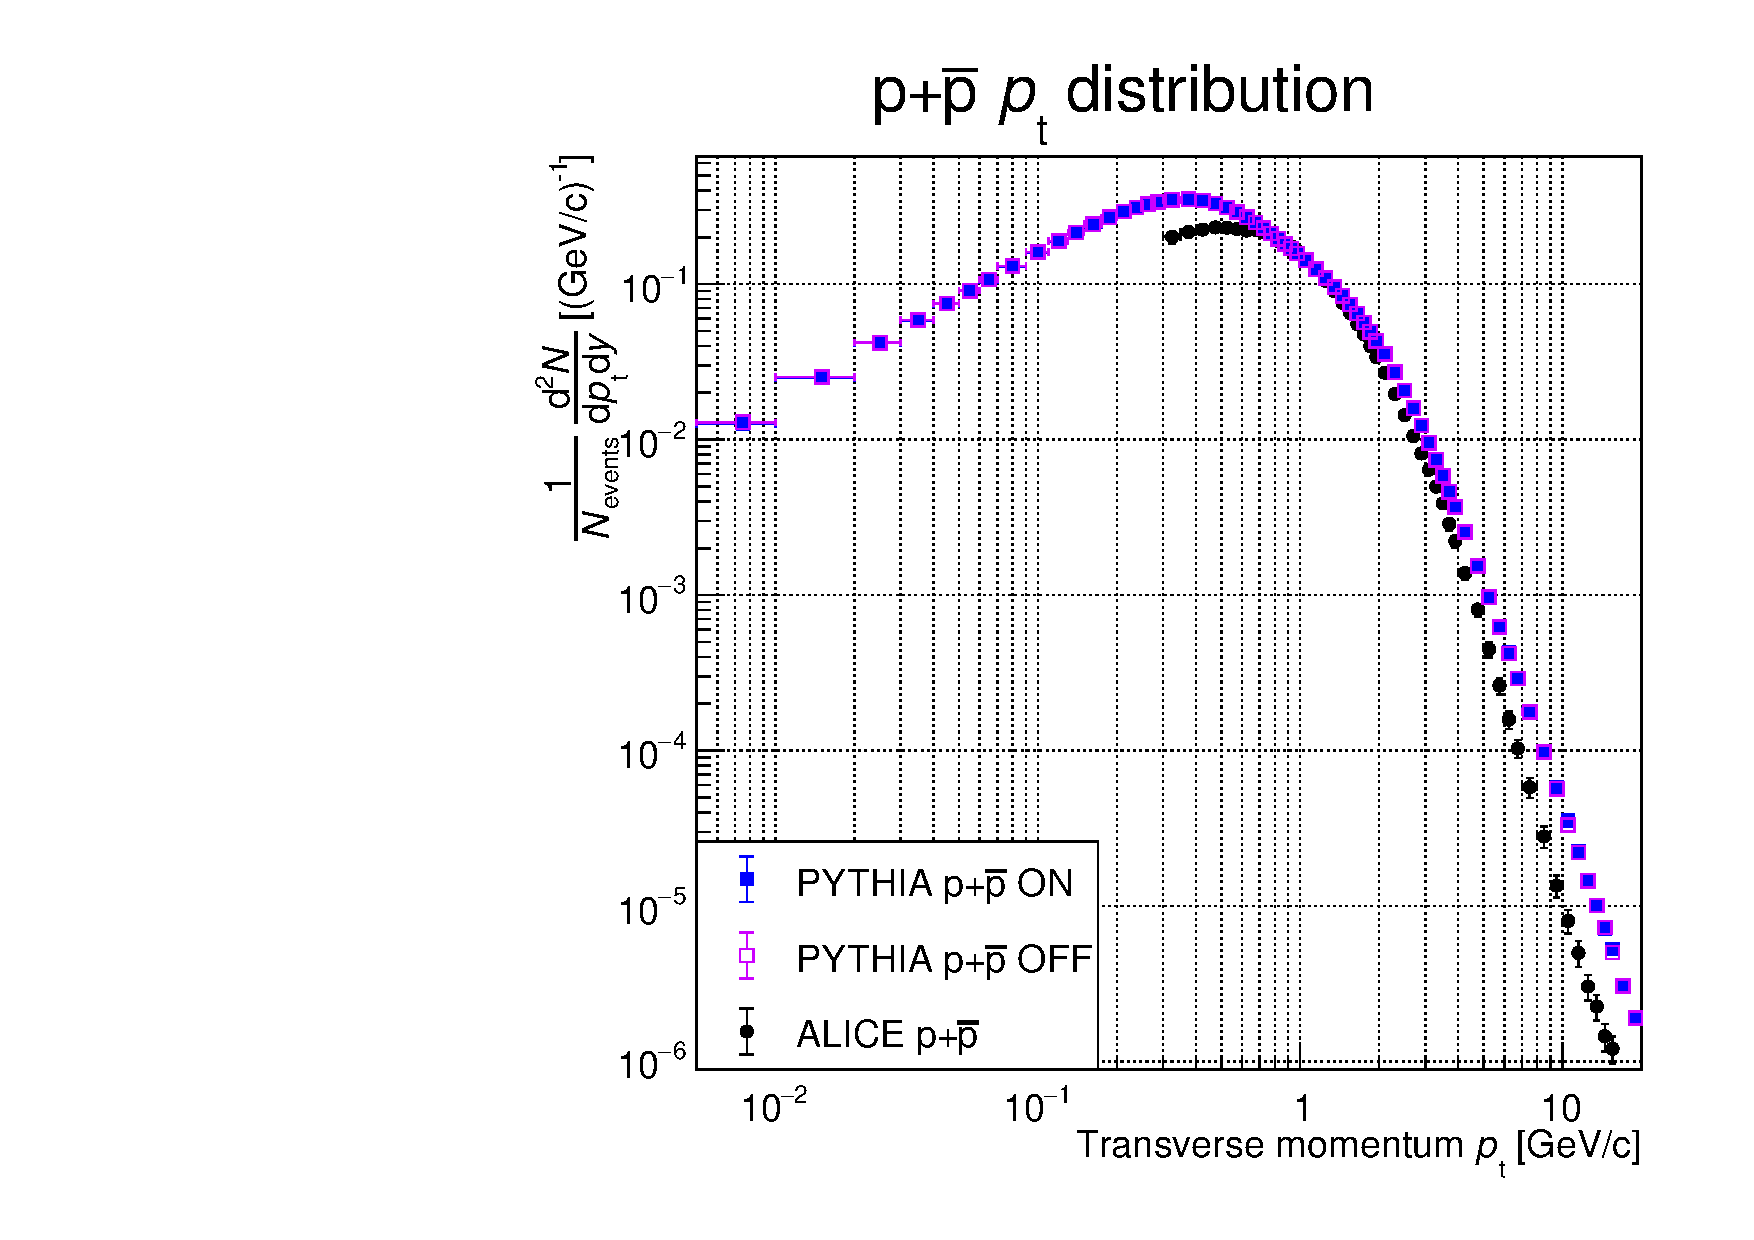
\includegraphics[width=\textwidth]{image/3-risultati/analyse/E/pp.pdf}
        \caption{}
        \label{fig:E_pp}
    \end{subfigure}
    %\hspace{1cm}
    \begin{subfigure}{.49\textwidth}
        \centering
        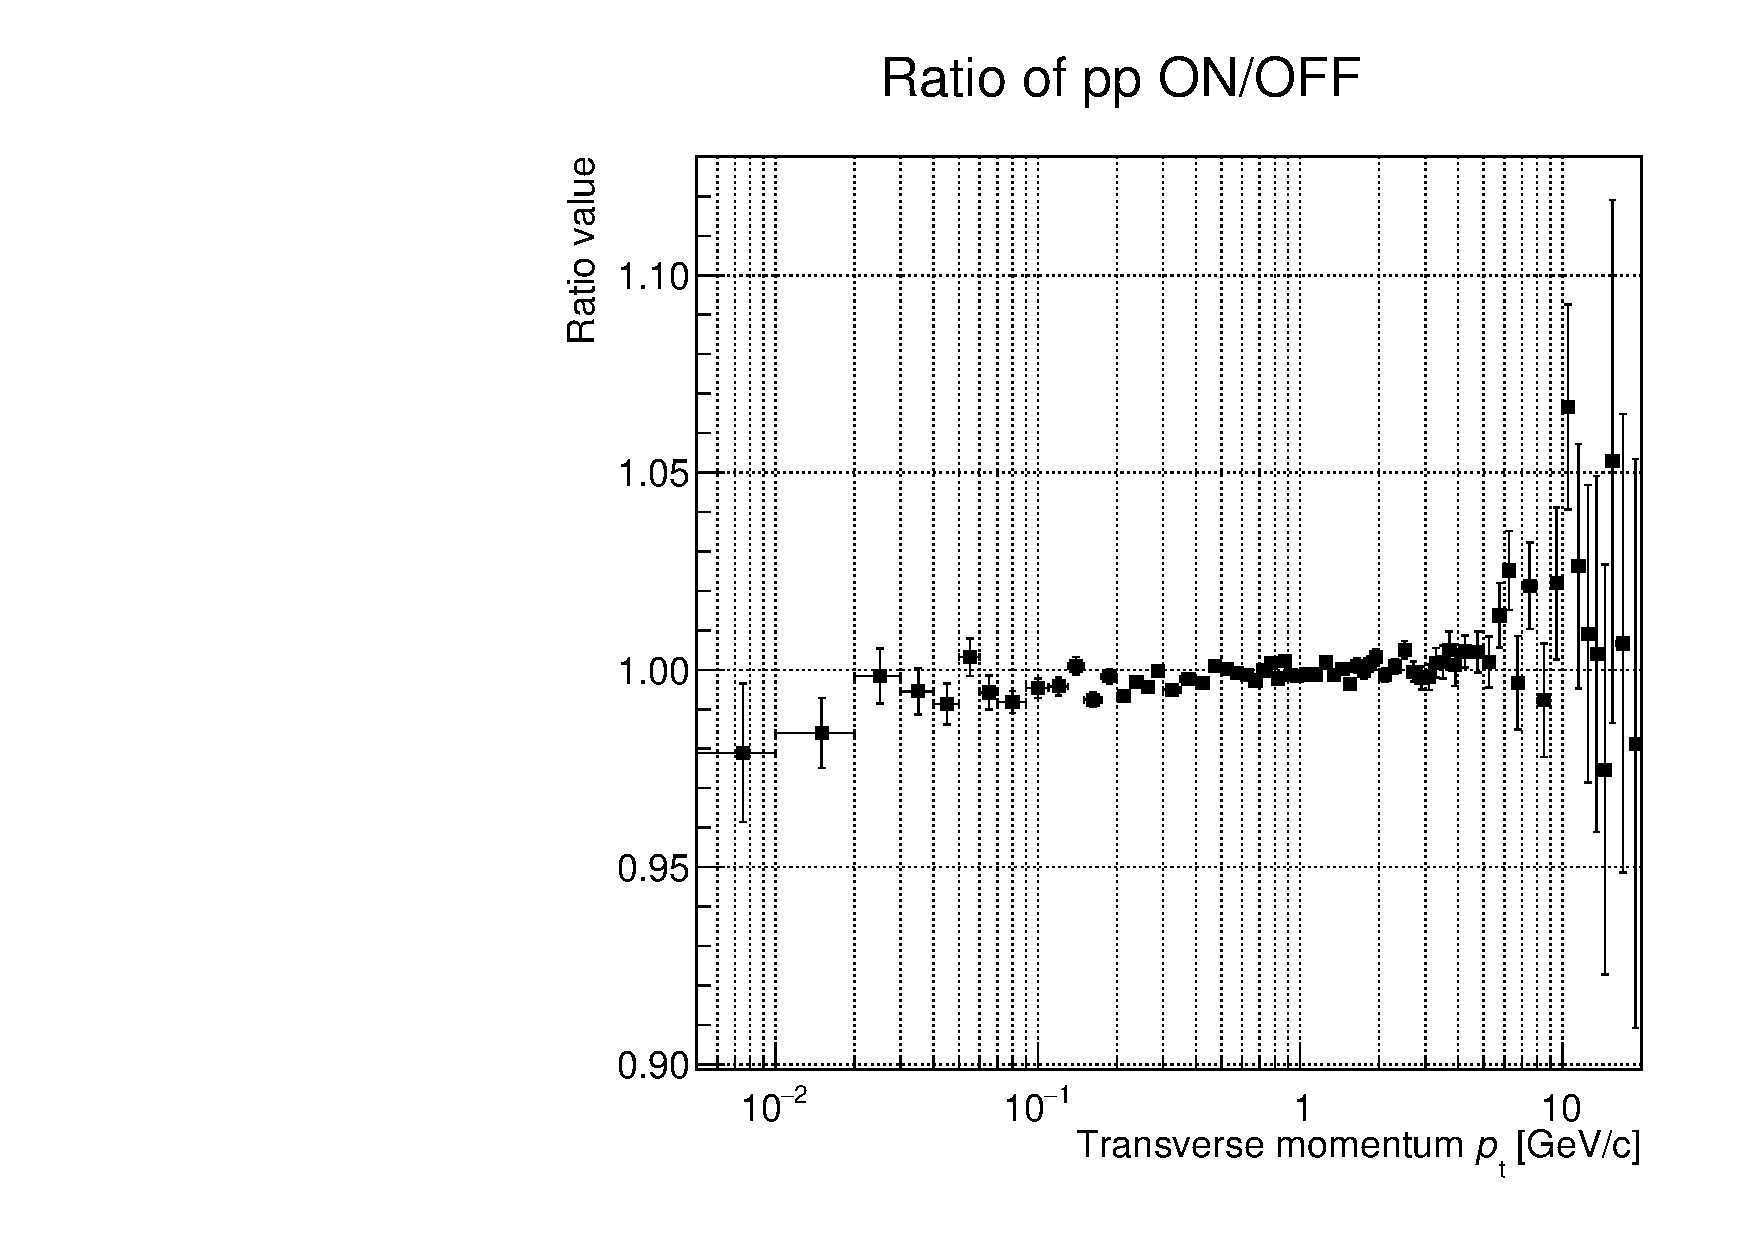
\includegraphics[width=\textwidth]{image/3-risultati/analyse/E/ratio_pp_ON_OFF.pdf}
        \caption{}
        \label{fig:E_ratio_pp_ON_OFF}
    \end{subfigure}
    \captionwithsource{\emph{\rmfamily (a)} Distribuzione dell'impulso trasverso di $p+\bar p$ con produzione deuteronica attivata e disattivata ("ON" e "OFF") in confronto con i dati sperimentali di ALICE ("ALICE"), usando il modello di coalescenza. \emph{\rmfamily (b)} Frazione della distribuzione dell'impulso trasverso di $p+\bar p$ con produzione deuteronica attivata e con produzione non attivata, usando il modello di coalescenza.}{\cite{ALICE:2020jsh}}
    \label{fig:E_pp_prod}
\end{figure}
Neanche la divisione tra il caso in cui la produzione deuteronica sia attivata e quella disattivata presenta particolari differenze, come si può notare in \autoref{fig:E_ratio_pp_ON_OFF}, con un valore della media pesata di $0.99873 \pm 0.00023$, vicino al valore di 0.999.

Invece gli spettri di produzione dei (anti)deuteroni (\autoref{fig:E_(anti)deuteron}) hanno un andamento diverso, come deve essere, visto che i diversi modelli utilizzati sono differenti.
Da questi grafici si osserva un andamento discordante degli spettri per tutto il dominio dei dati di ALICE, sottolineando l'inadeguatezza del modello di coalescenza. 
Eseguendo una divisione tra i dati dei (anti)deuteroni di \pythia{} e di ALICE otteniamo il grafico riportato in \autoref{fig:E_division} ed eseguendo una media pesata del rapporto otteniamo il valore di $0.793 \pm 0.012$ per i deuteroni e $0.738 \pm 0.016$ per gli antideuteroni, quindi una sottoproduzione di circa 20-30\%.\\

Come verifica ulteriore della correttezza delle predizioni è stato misurato il rapporto tra gli istogrammi dei deuteroni e degli antideuteroni (\autoref{fig:E_ratio_DD}), ottenendo un valore della media pesata di $1.008 \pm 0.008$, compatibile con il valore unitario.\\

Ora, eseguendo invece una divisione tra il modello di coalescenza e il modello predefinito di \pythiaa{}, si ottiene il grafico visibile in \autoref{fig:A_vs_E}.
I due modelli presentano un andamento simile solamente nel range tra $0.1-1$ GeV/$c$, in cui per entrambi si è osservato una sovrapproduzione di (anti)deuteroni rispetto ai dati di ALICE.
\begin{figure}[htbp]
    \centering
    \begin{subfigure}{.49\textwidth}
    \centering
        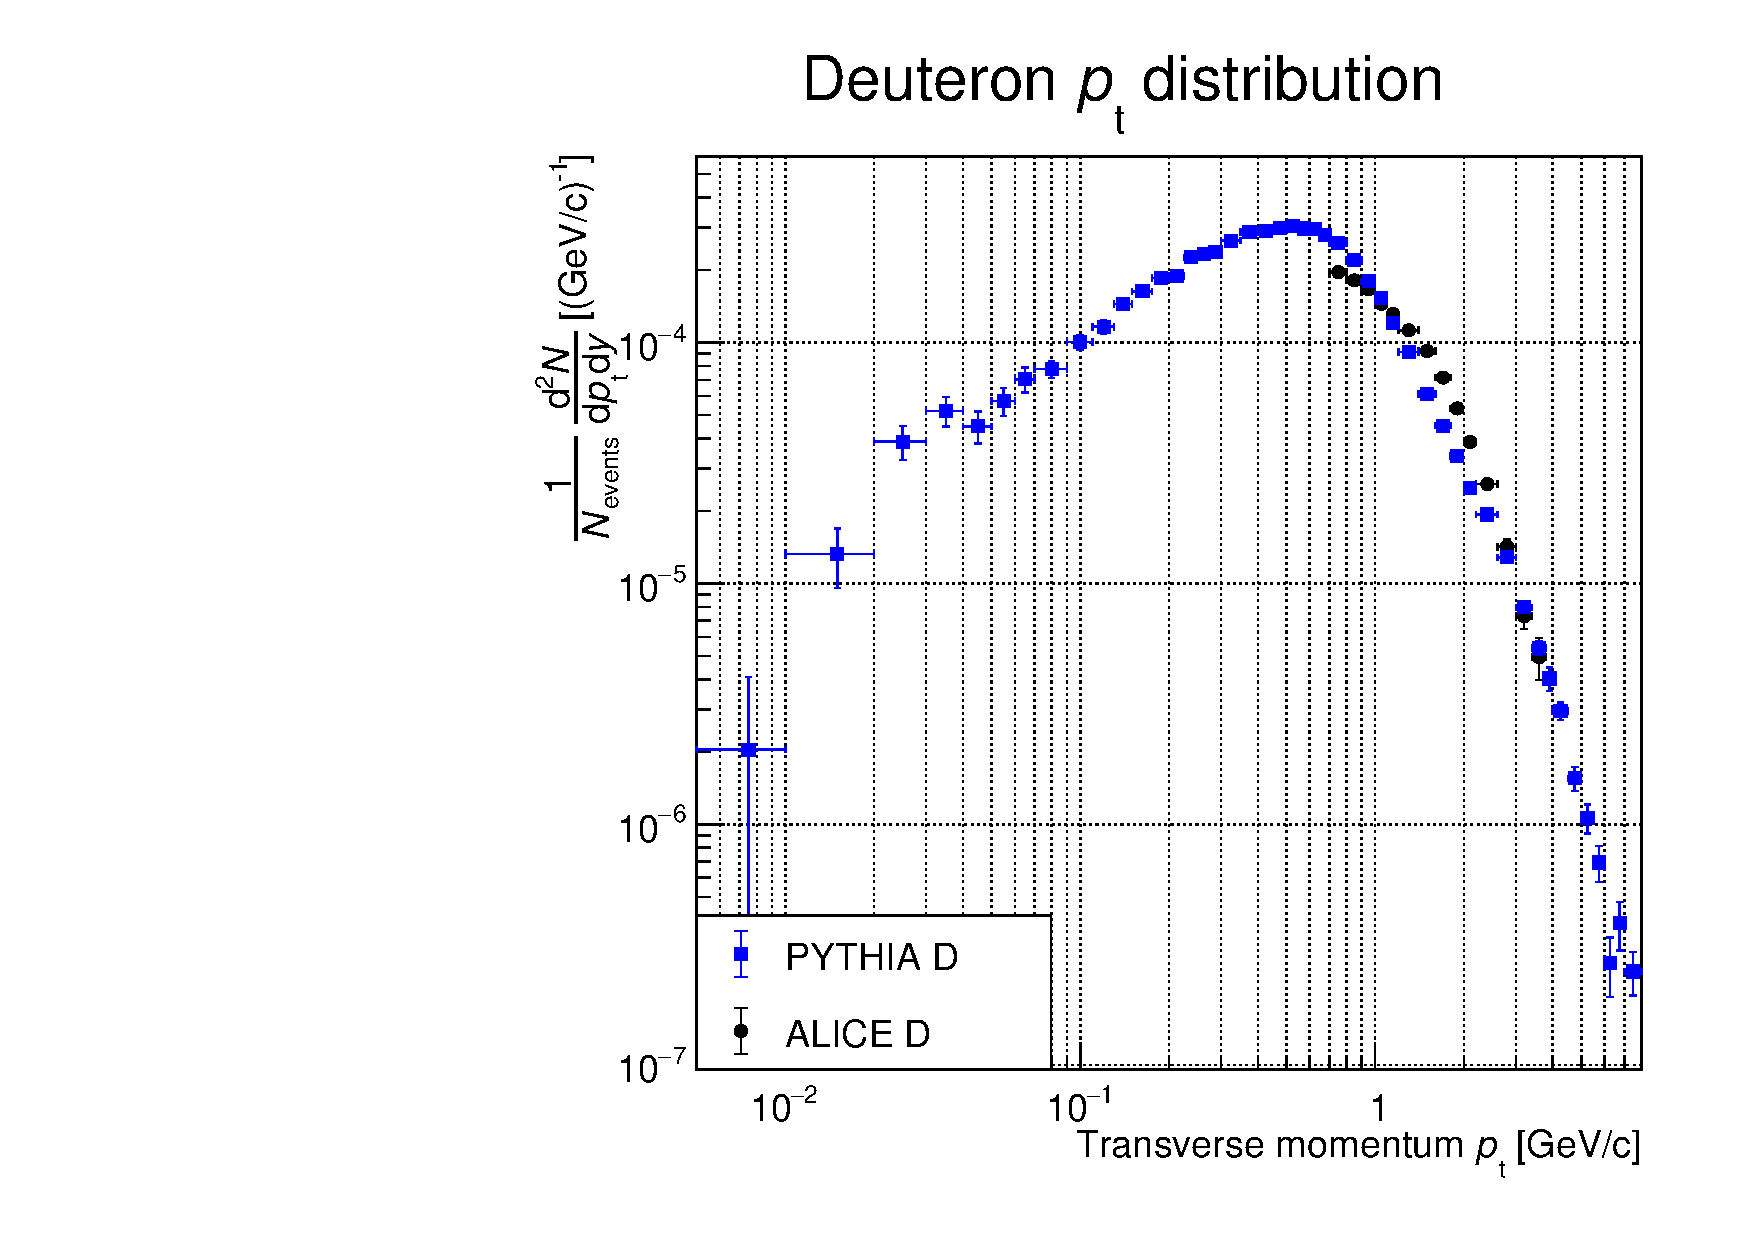
\includegraphics[width=\textwidth]{image/3-risultati/analyse/E/deuteron.pdf}
        \caption{}
        \label{fig:E_deuteron}
    \end{subfigure}
    %\hspace{1cm}
    \begin{subfigure}{.49\textwidth}
        \centering
        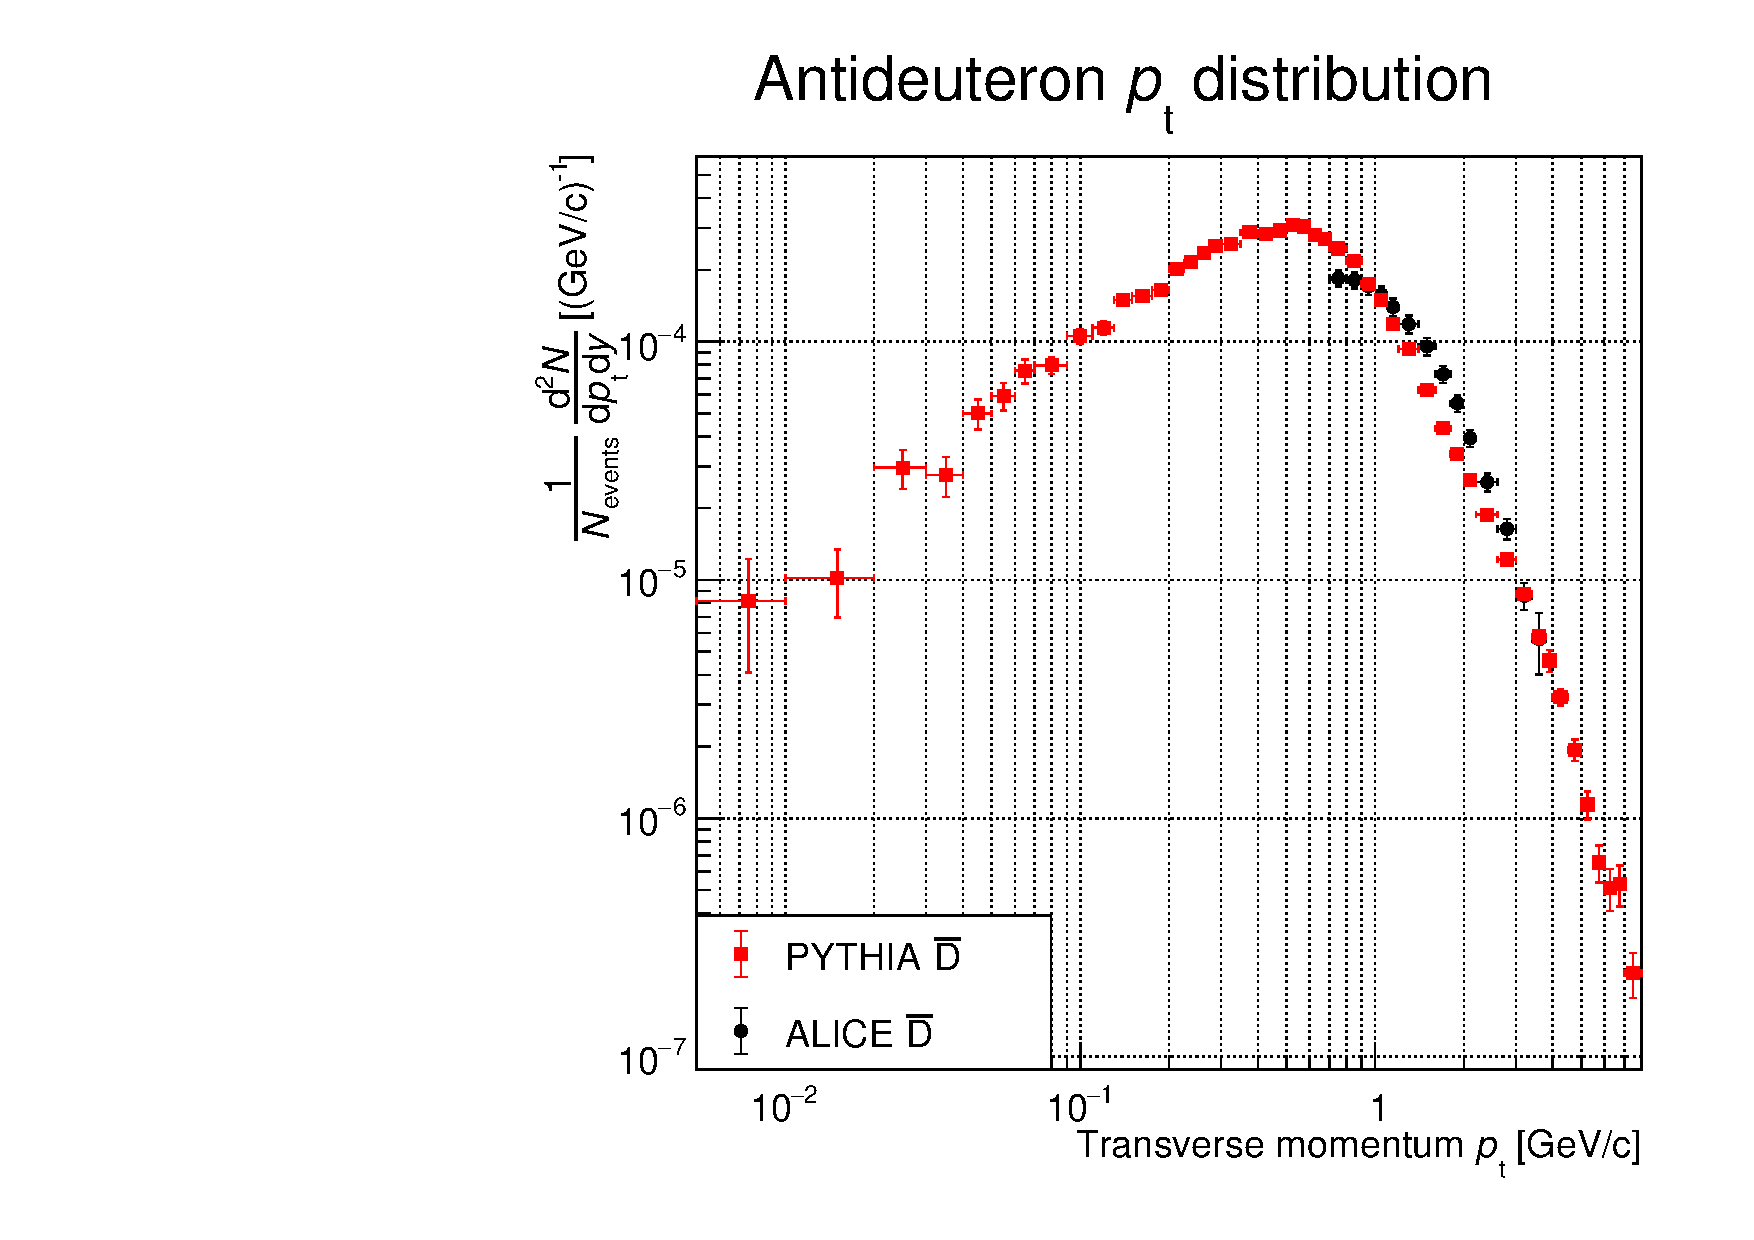
\includegraphics[width=\textwidth]{image/3-risultati/analyse/E/antideuteron.pdf}
        \caption{}
        \label{fig:E_antideuteron}
    \end{subfigure}
    \captionwithsource{Distribuzione dell'impulso trasverso di \emph{\rmfamily (a)} $D$ e \emph{\rmfamily (b)} di $\bar D$ in confronto con i dati di ALICE, utilizzando il modello di coalescenza.}{\cite{ALICE:2020foi}}
    \label{fig:E_(anti)deuteron}
\end{figure}
\begin{figure}[htbp]
    \centering
    \begin{subfigure}{.49\textwidth}
    \centering
        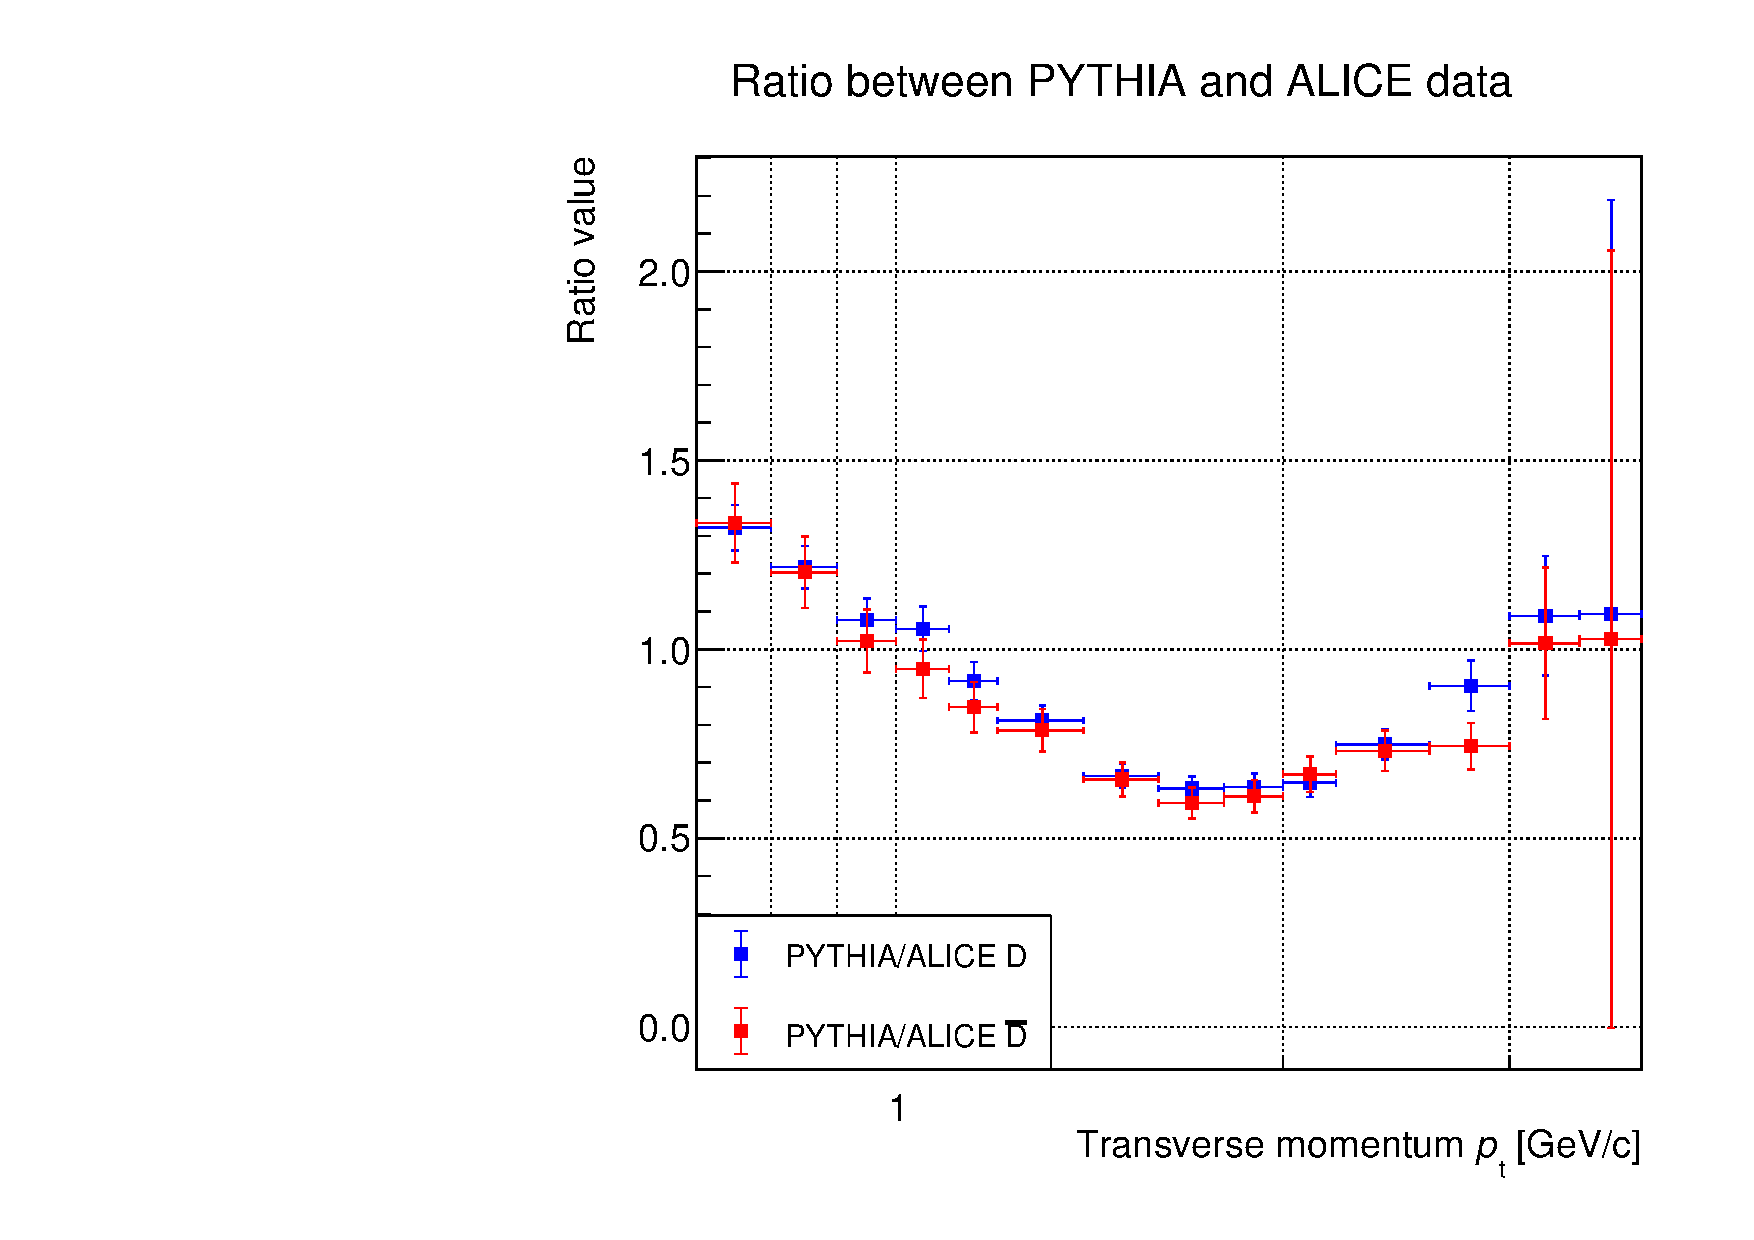
\includegraphics[width=\textwidth]{image/3-risultati/analyse/E/division.pdf}
        \caption{}
        \label{fig:E_division}
    \end{subfigure}
    %\hspace{1cm}
    \begin{subfigure}{.49\textwidth}
        \centering
        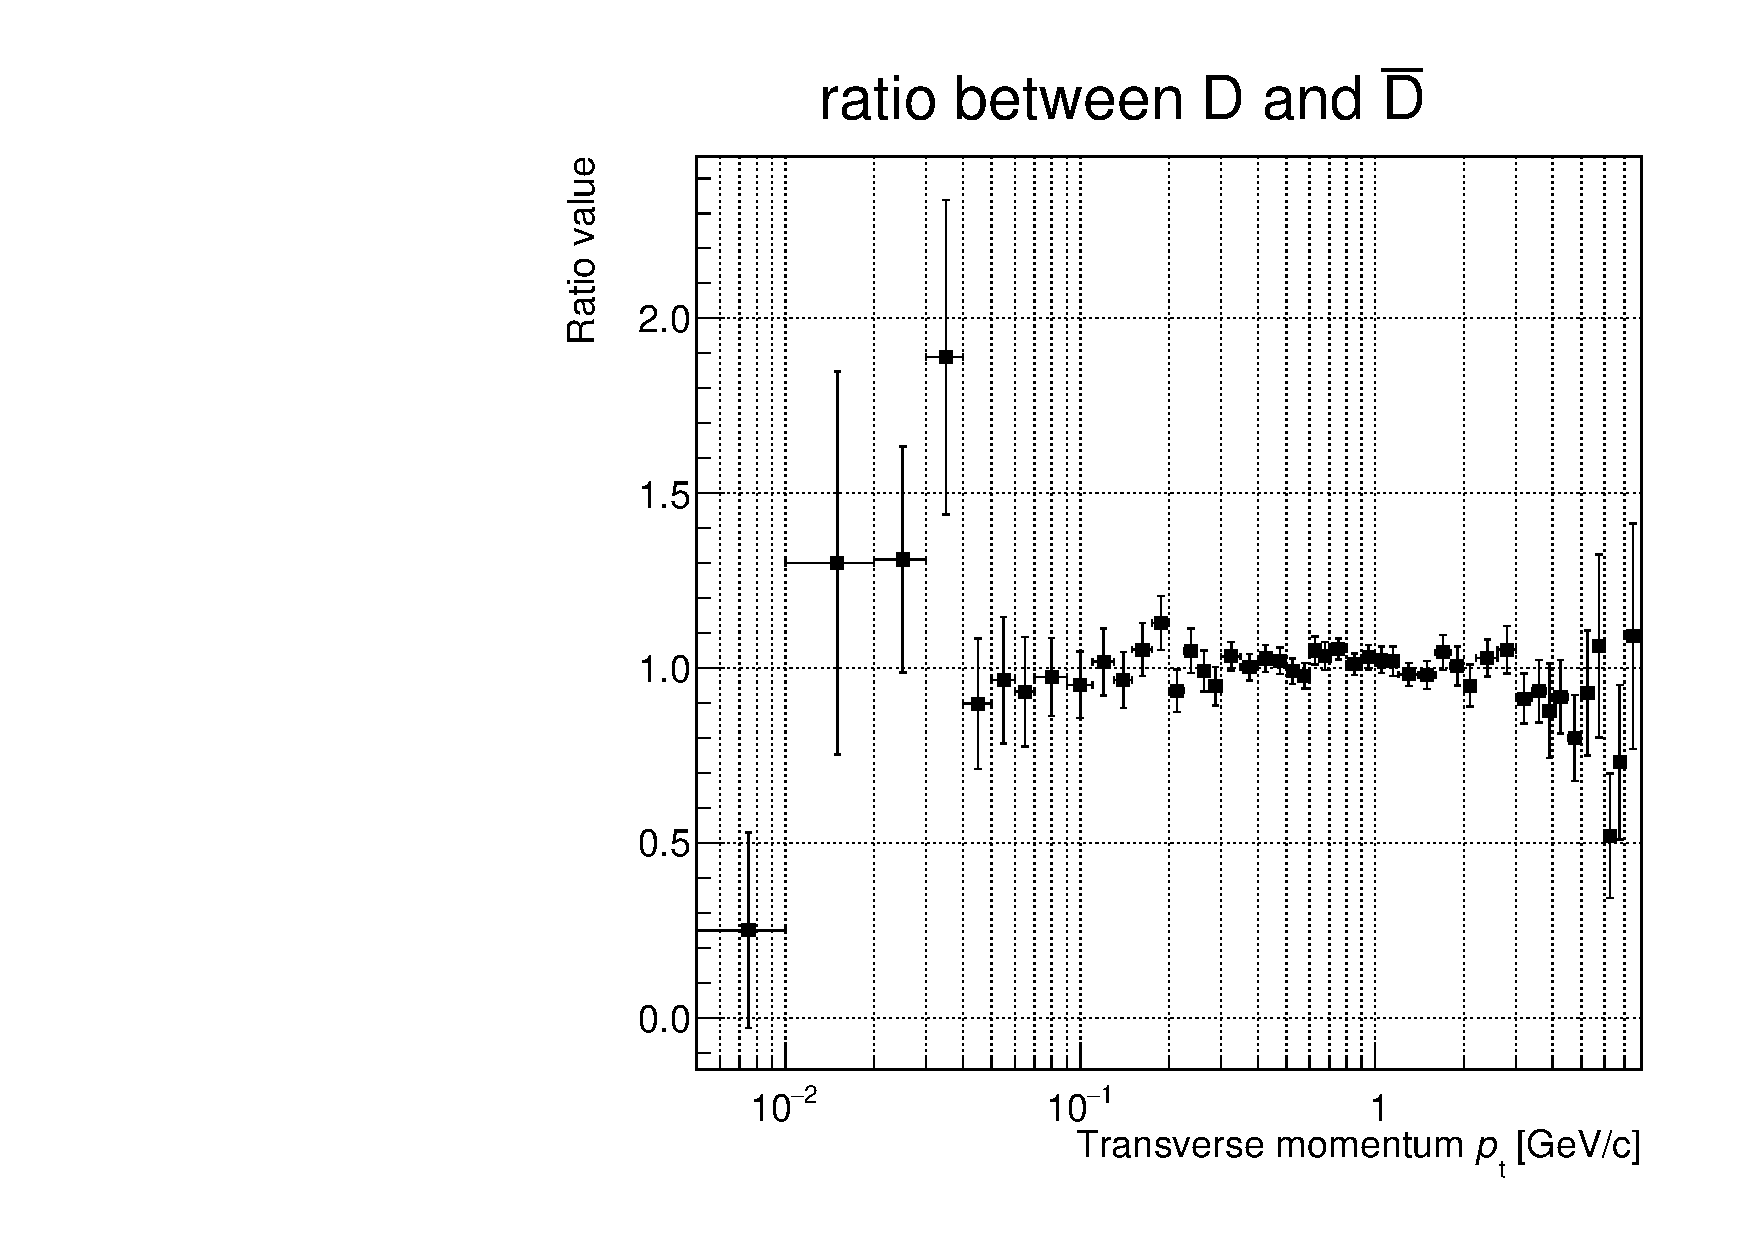
\includegraphics[width=\textwidth]{image/3-risultati/analyse/E/ratio_DD.pdf}
        \caption{}
        \label{fig:E_ratio_DD}
    \end{subfigure}
    \caption{\emph{\rmfamily (a)} Divisione tra la distribuzione dell'impulso trasverso di $D$ e $\bar D$ con i dati di ALICE, utilizzando il modello di coalescenza. \emph{\rmfamily (b)} Frazione delle distribuzione dell'impulso trasverso di $D$ con quello di $\bar D$, utilizzando il modello di coalescenza.}
    \label{fig:E_ratio_DD_}
\end{figure}
\begin{figure}[htp]
    \centering
    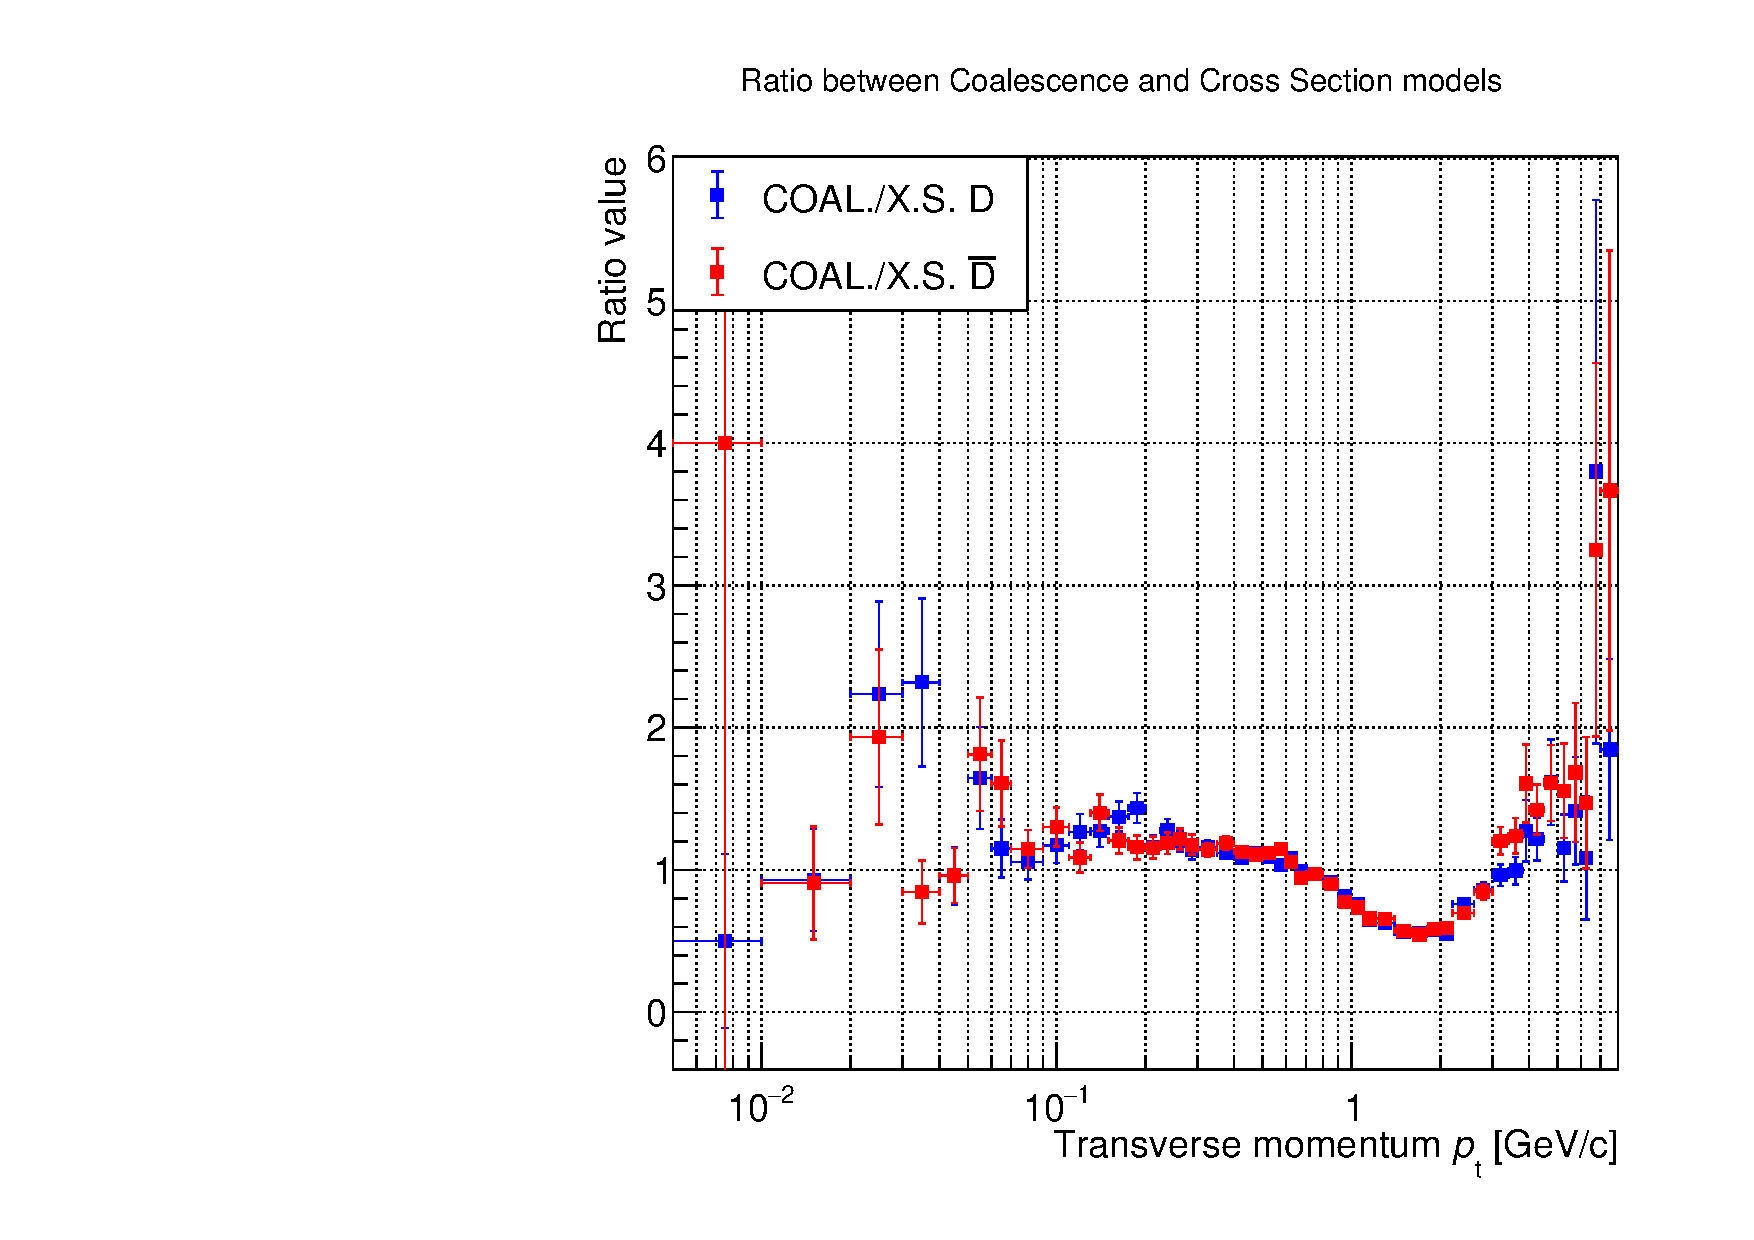
\includegraphics[width=0.49\textwidth]{image/3-risultati/analyse/A/ratio_CXS.pdf}
    \caption{Rapporto tra la distribuzione dell'impulso trasverso di $D$ e $\bar D$ ottenuta con il modello di coalescenza e con il modello predefinito di \emph{\pythiaa}. "COAL" indica il modello di coalescenza, "X.S." indica il modello di \pythiaa{}.}
    \label{fig:A_vs_E}
\end{figure}
%%%%%%%%%%%%%%%%%%%%%%%%%%%%%%%%%%%%%%%%%%
\section{Ottimizzazione del modello di PYTHIA}
Il lavoro principale di questa tesi è stato quello di andare a ottimizzare il parametro \ttbox{norm}.
Originariamente il gruppo di \pythiaa{} aveva calcolato questo parametro scegliendo il valore di $1/\sigma_0$ con energia di centro di massa $\sqrt s = 7$ TeV per il caso dei deuteroni, ossia $1/\sigma_0 = 2.63$ \si{barn^{-1}} (si veda la \autoref{tab:valori_p0_1sigma0}).
Questo dovrebbe spiegare gli andamenti dei grafici in \autoref{fig:A_(anti)deuteron} che non riproducono fedelmente quelli di ALICE.
Quindi si è andati a prendere in considerazione la \autoref{tab:valori_p0_1sigma0} e a cercare di determinare il valore di $1/\sigma_0$ corrispondente a una energia del centro di massa $\sqrt s = 13$ TeV.
Visto che le impostazioni predefinite hanno prodotto una sovrapproduzione, allora vuol dire che $1/\sigma_0$ ha assunto un valore troppo alto per $\sqrt s = 13$ TeV.
Ciò è supportato dal fatto che $1/\sigma_0$ ha un andamento decrescente nella \autoref{tab:valori_p0_1sigma0}.
Quindi l'obiettivo è stato quello di estrapolare questo parametro dalla tabella in questione, facendo attenzione al numero ridotto di punti che si ha a disposizione.

\subsubsection{Fit lineare}
Un primo approccio è stato quello di effettuare un fit lineare ai dati del deuterone per cercare di ottenere un valore preliminare tramite il quale andare a raffinare il parametro.
Tramite questo fit lineare (\autoref{fig:fit_norm}) l'estrapolazione di $1/\sigma_0$ a $\sqrt{s} = 13$ TeV fornisce un valore di $1.7136$ \si{barn^{-1}}, con un valore di $\ttbox{norm} = 183.56$.
\begin{figure}[htb]
    \centering
    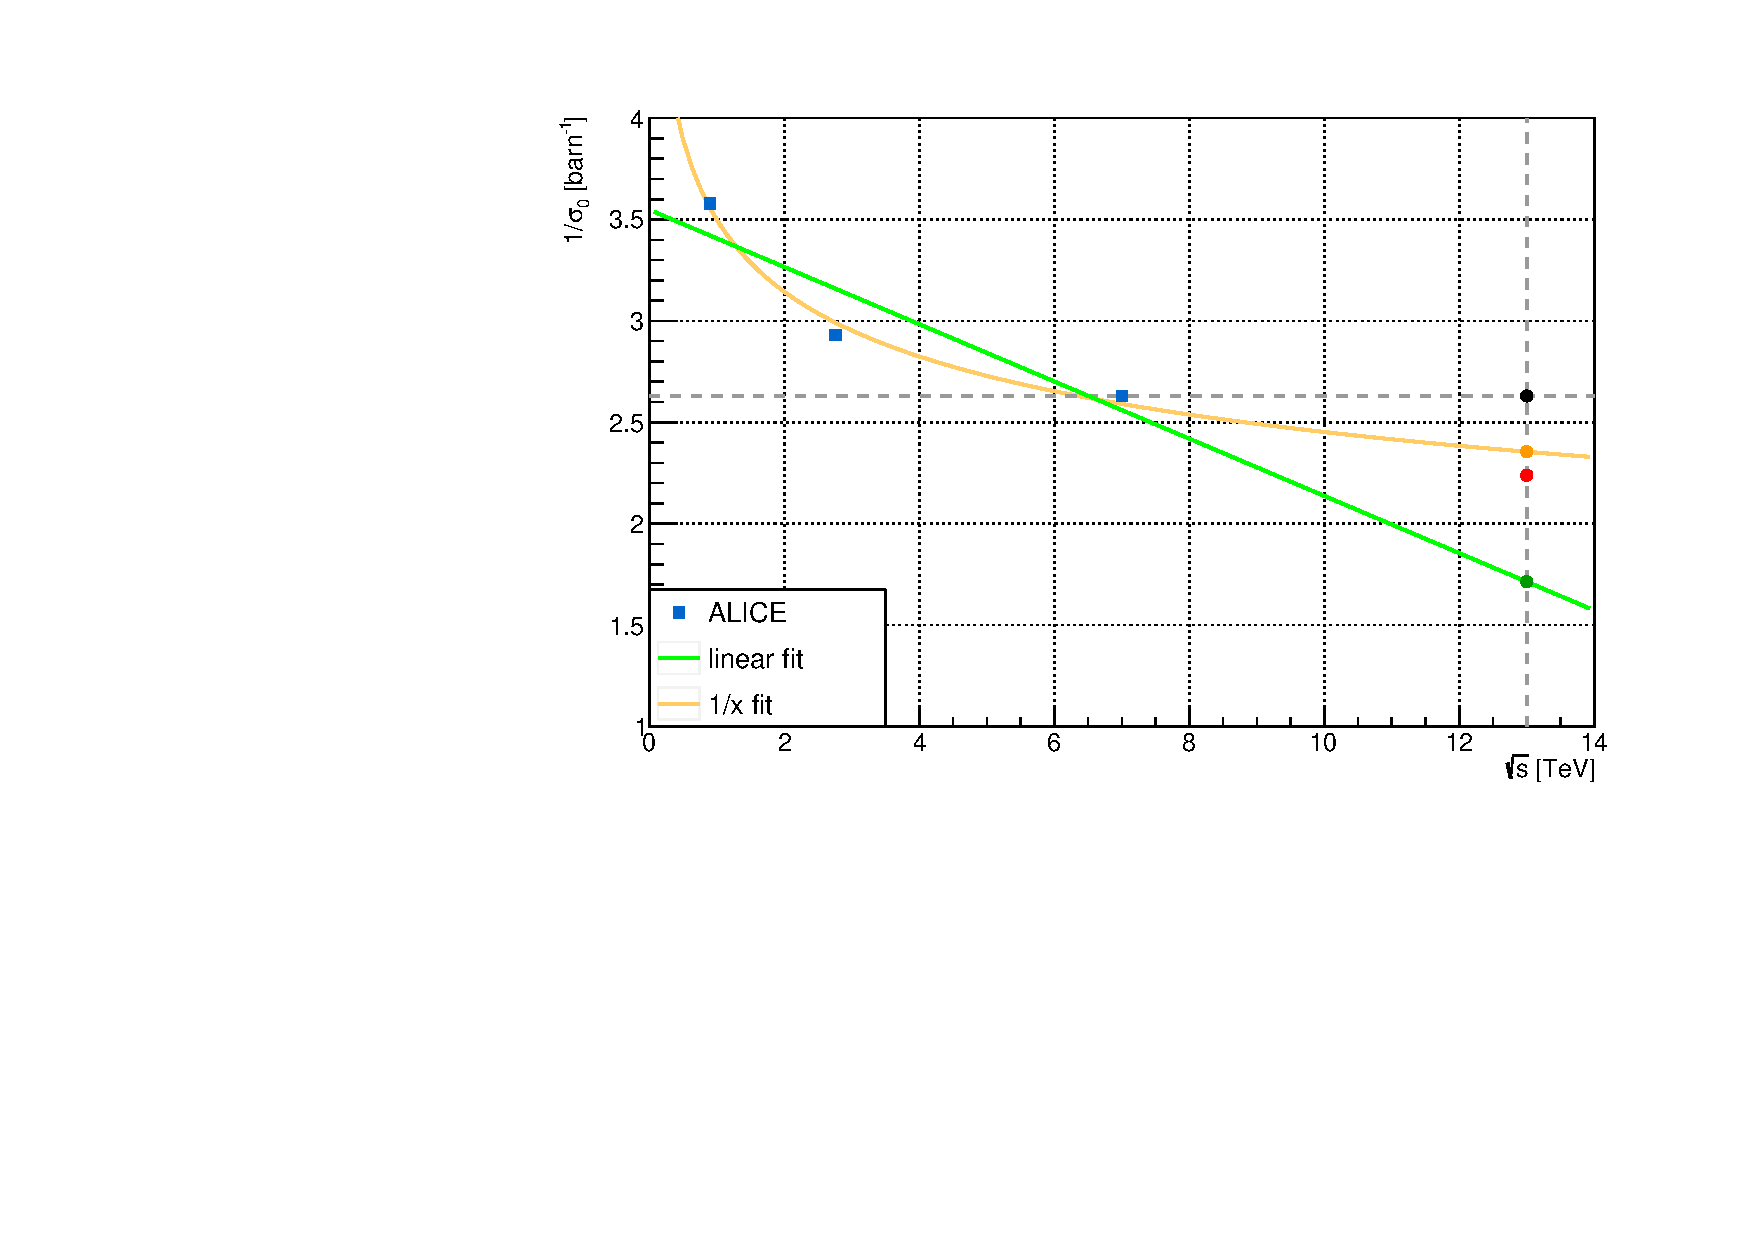
\includegraphics[width=0.9\textwidth]{image/canvas.pdf}
    \caption{Risultati del fit lineare e $1/x$ del parametro $1/\sigma_0$ per i deuteroni. La retta tratteggiata in orizzontale rappresenta $1/\sigma_0 = 2.63$ \si{barn^{-1}}, quella verticale $\sqrt s = 13$ TeV. Su quest'ultima vi sono quattro punti, che in ordine rappresentano (dall'alto verso il basso) il parametro default, del fit $1/x$, ottimizzato e del fit lineare.
    "ALICE" indica i punti derivati da \autoref{tab:valori_p0_1sigma0} nella colonna dei deuteroni.}
    \label{fig:fit_norm}
\end{figure}
Per verificare l'attendibilità di questo valore si è andati a effettuare una simulazione con questo valore di \ttbox{norm} e a confrontare lo spettro di produzione dei (anti)deuteroni con quelli di ALICE.
Le medie pesate derivate dai rapporti tra i dati di \pythiaa{} e di ALICE (in \autoref{fig:B_division}) hanno portato a un valore di $0.789 \pm 0.012$ e $0.746 \pm 0.016$ rispettivamente per i deuteroni e per gli antideuteroni, indicando una sottoproduzione del circa 20-25\%.
Da ciò si può dedurre che il valore $1/\sigma_0$ estrapolato tramite un fit lineare è inferiore rispetto al parametro ideale.
Un fit analogo del parametro $1/\sigma_0$ per gli antideuteroni ha fornito un valore di $1.56872$ \si{barn^{-1}}, corrispondente a $\ttbox{norm} = 200.51$, che tuttavia risulta troppo alto visto il risultato della simulazione con $\ttbox{norm} = 183.56$; tale valore perciò non è stato considerato.

\subsubsection{Fit ${\bf 1/x}$}
Un secondo approccio più realistico è stato quello di tentare di fittare i tre punti con una funzione del tipo
\begin{equation}
    1/\sigma_0\left(\sqrt s\right) = \dfrac{a}{x^b}
\end{equation}
Eseguendo il fit (\autoref{fig:fit_norm}) con questa funzione si è riusciti a ottenere i seguenti valori dei parametri di fit: $a = (3.50 \pm 0.07)$ \si{barn^{-1}} e $b = 0.154 \pm 0.017$.
Così il valore di $1/\sigma_0$ estrapolato a $\sqrt s = 13$ TeV risulta essere di $2.35473$ \si{barn^{-1}}, quindi $\ttbox{norm} = 133.58$, valore accettabile perché compreso tra 119.6 e 183.56.
Eseguendo le simulazioni Monte Carlo con questo parametro si ottiene che gli andamenti degli spettri dei (anti)deuteroni si avvicinano di più ai dati di ALICE rispetto alle simulazioni precedenti.
\begin{figure}[h]
    \centering
    \begin{subfigure}{.49\textwidth}
    \centering
        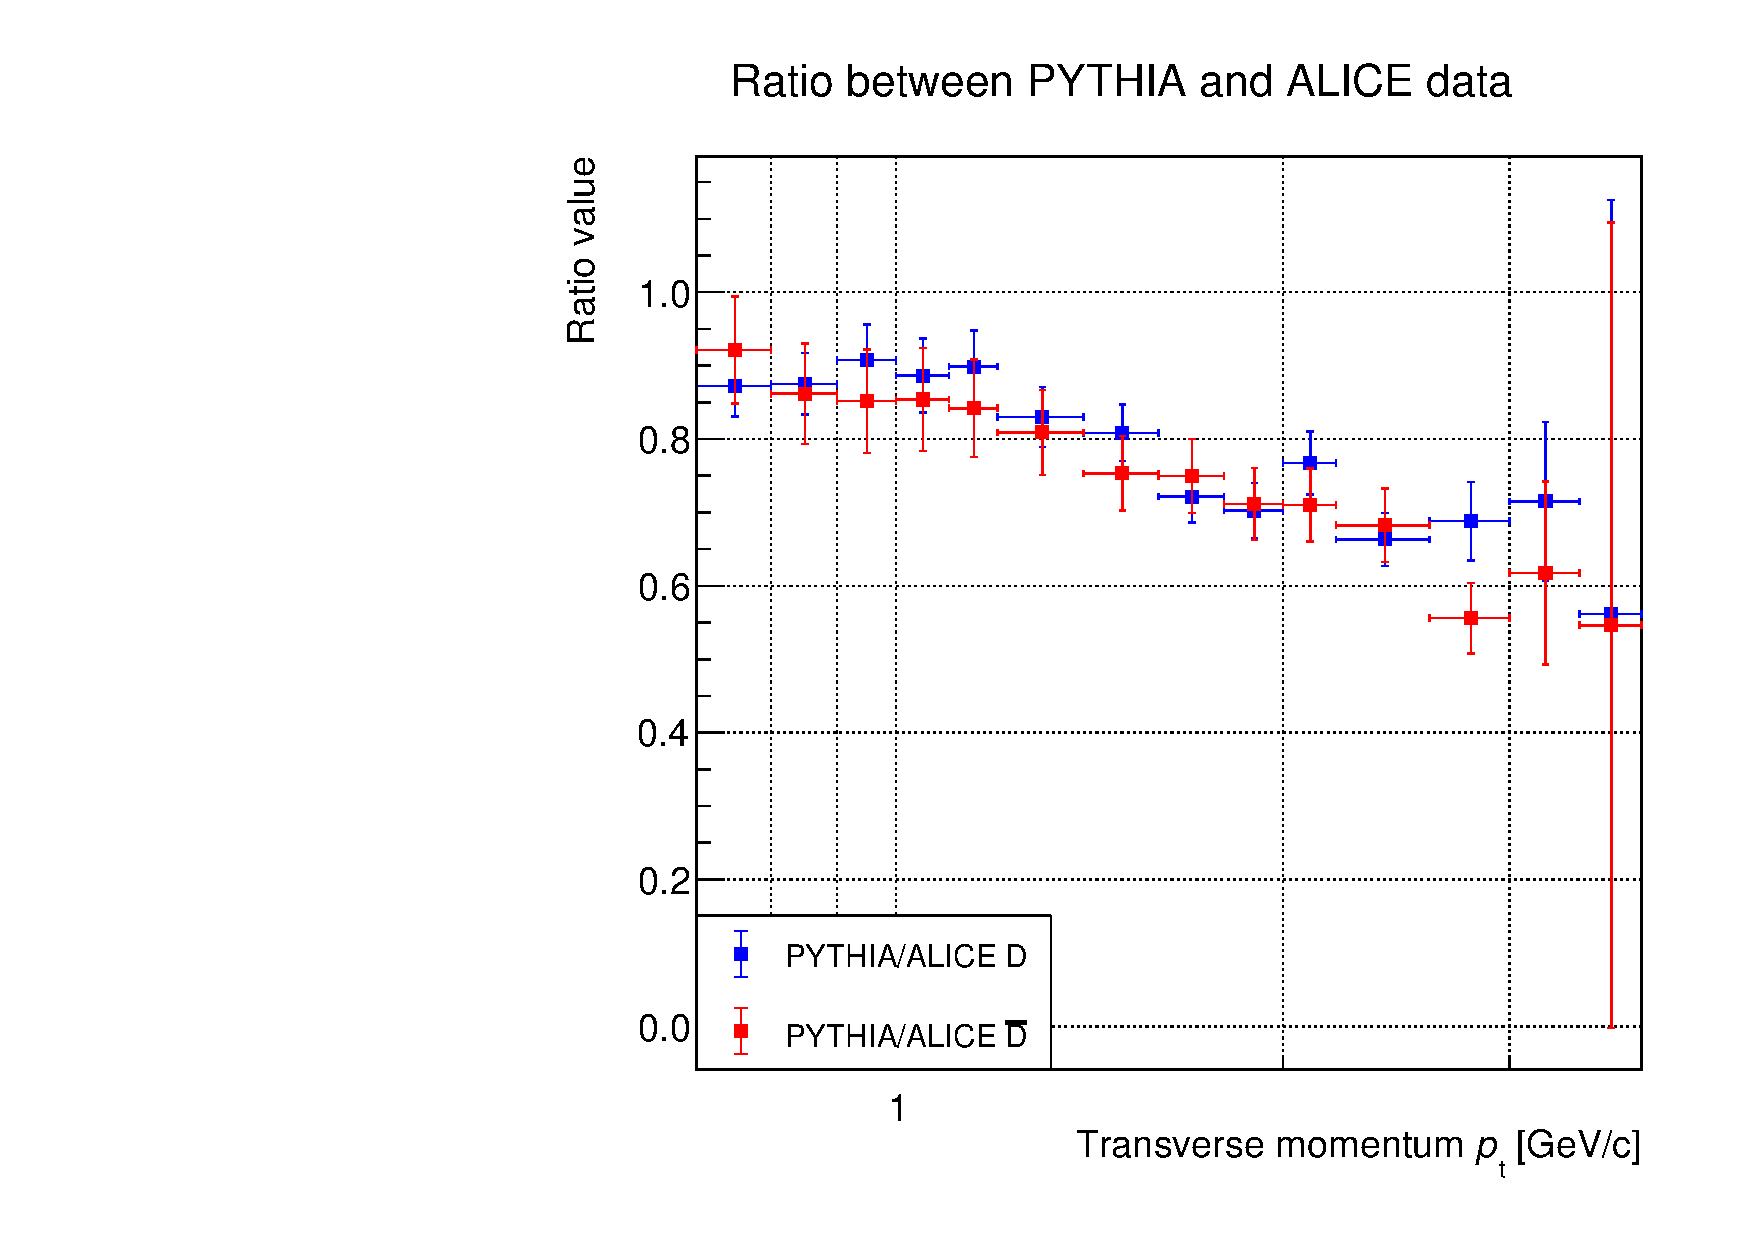
\includegraphics[width=\textwidth]{image/3-risultati/analyse/B/division.pdf}
        \caption{}
        \label{fig:B_division}
    \end{subfigure}
    %\hspace{1cm}
    \begin{subfigure}{.49\textwidth}
        \centering
        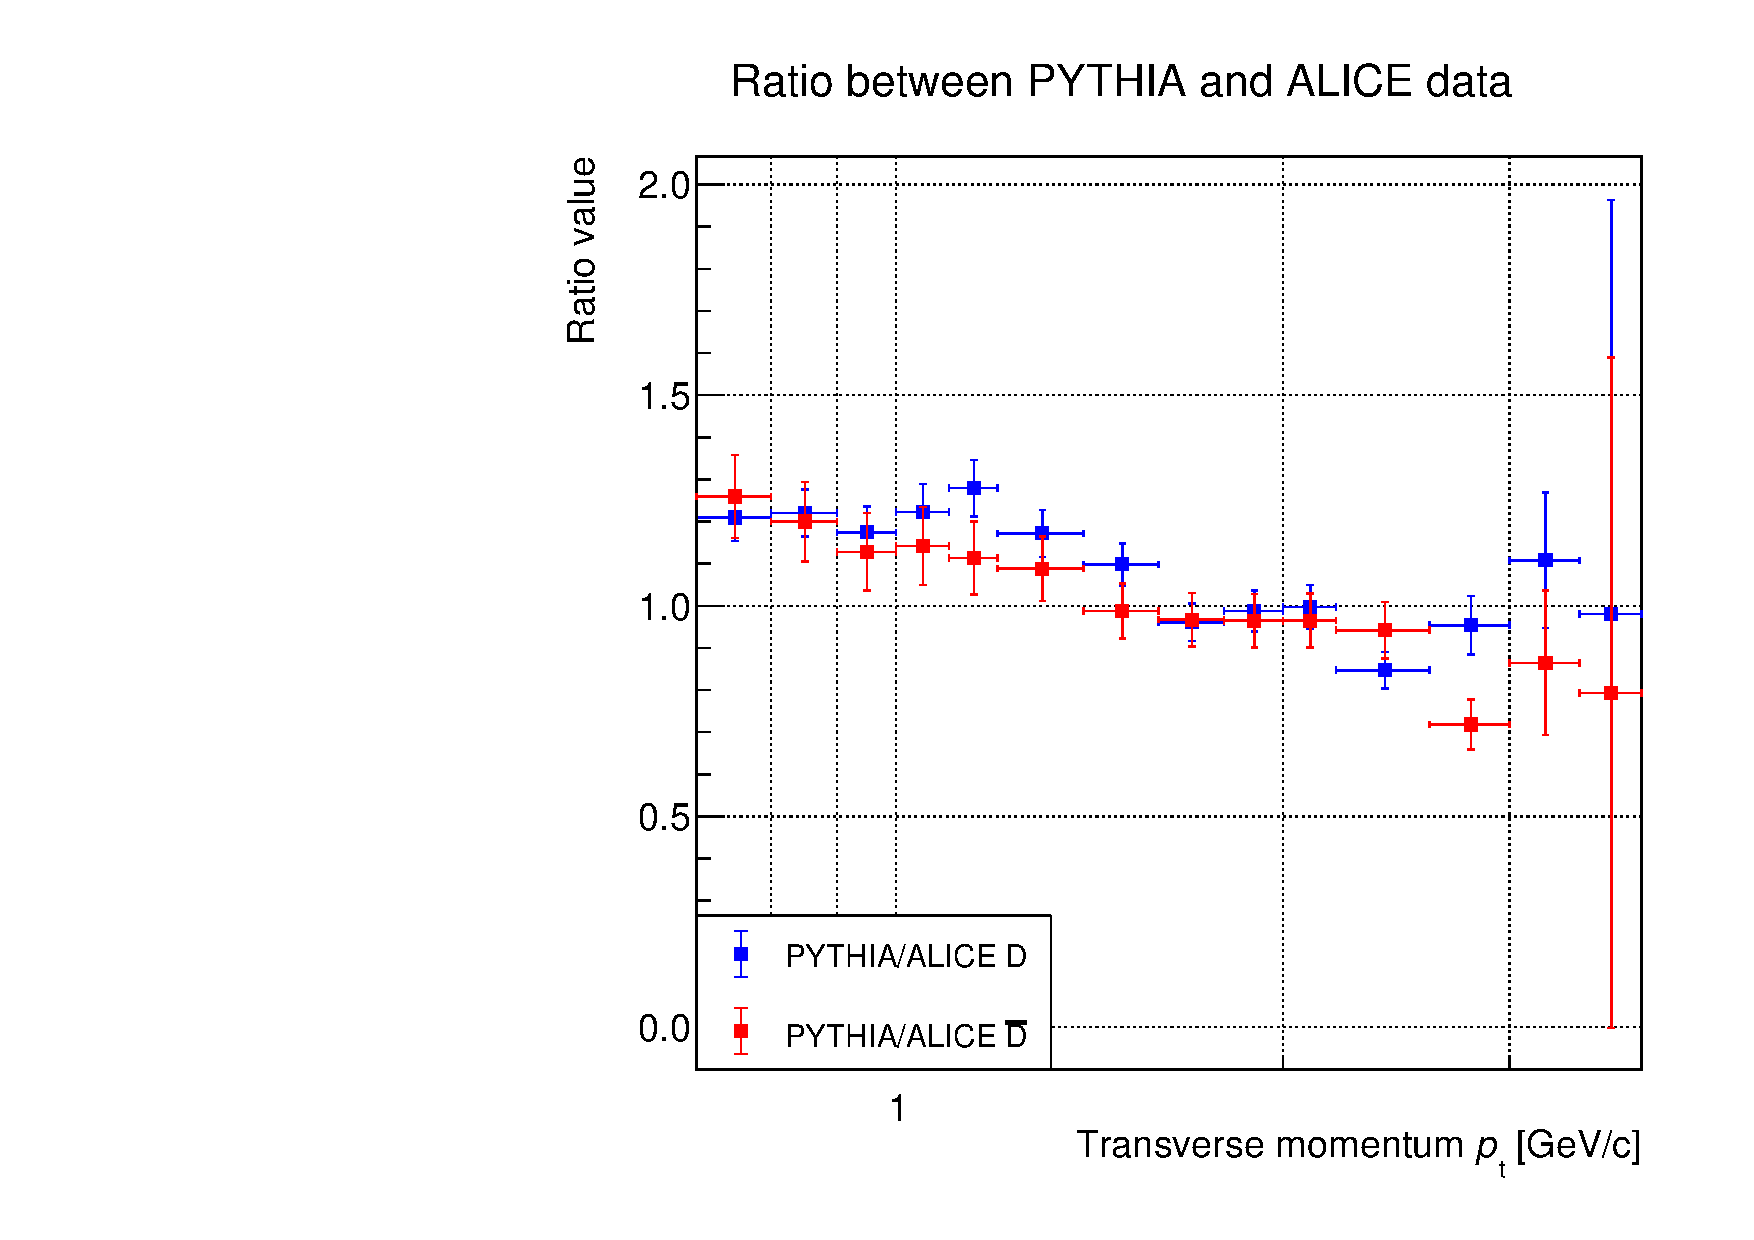
\includegraphics[width=\textwidth]{image/3-risultati/analyse/F/division.pdf}
        \caption{}
        \label{fig:F_division}
    \end{subfigure}
    \caption{Rapporto tra la distribuzione dell'impulso trasverso di $D$ e $\bar D$ con i dati di ALICE \emph{\rmfamily (a)} con \emph{\ttbox{norm}}$=183.56$ e \emph{\rmfamily (b)} con \emph{\ttbox{norm}}$=133.58$.}
    \label{fig:ratio_pp_ON_OFF_BF}
\end{figure}
Questo è supportato dal valore della media pesata del rapporto tra lo spettro dei (anti)deuteroni con i dati di ALICE (\autoref{fig:F_division}) che vale $1.067 \pm 0.015$ e di $0.993 \pm 0.021$ rispettivamente per i deuteroni e per gli antideuteroni. Quindi si nota che il valore di \ttbox{norm} per gli antideuteroni risulta già compatibile entro gli errori con il valore unitario, ma non per i deuteroni.
Questo valore del parametro potrebbe apparire come valore  ottimale, ma ricordando che i valori considerati della \autoref{tab:valori_p0_1sigma0} si riferiscono solamente ai deuteroni, perciò si è proseguiti con l'ottimizzazione del parametro.

\subsubsection{Bisezione}
Per trovare un valore del parametro \ttbox{norm} tale da soddisfare sia la produzione di deuteroni e antideuteroni si è proceduti con un altro metodo alternativo, ispirato al metodo di bisezione.
Per far ciò si correla il parametro \ttbox{norm} con la relativa media pesata.
Andando a considerare i punti del modello predefinito ($\ttbox{norm} = 119.6$, media pesata $= 1.203 \pm 0.017$) e del fit $1/x$ ($\ttbox{norm} = 133.58$, media pesata $= 1.067 \pm 0.03$), si è andati a stimare il valore ottimale del parametro eseguendo empiricamente un fit lineare dei due punti e ricavare il valore del parametro quando la media assume un valore di 1.
Utilizzando questo approccio si è giunti al valore del parametro di $\ttbox{norm} = 140.46721$, leggermente inferiore al parametro derivato dal fit $1/x$.
Eseguendo le simulazioni Monte Carlo ed effettuando il rapporto tra le produzioni di (anti)deuteroni delle simulazioni e di ALICE, otteniamo i valori di media pesata di $1.036 \pm 0.015$ per i deuteroni e $ 0.939 \pm 0.020$ per gli antideuteroni.
Il valore della media pesata per i deuteroni è vicino a 1, ma non è compatibile entro gli errori.
Tuttavia, per semplicità assumiamo questo valore come valore ideale di \ttbox{norm}, e tramite una formula inversa ricaviamo un valore di $1/\sigma_0$ di 2.24 \si{barn^{-1}}.\\

È doveroso notare che, modificando il parametro \ttbox{norm}, quello che si va a fare non è altro che un un semplice riscalaggio agli spettri dei (anti)deuteroni, senza favorire un particolare canali di produzione della \autoref{tab:valori_p0_1sigma0}.
Per cui l'analisi dei canali (e dei loro subcanali) eseguita in \autoref{ch:channels} dovrebbe valere per tutti i valori di \ttbox{norm} (ignorando le regioni in cui si ha meno statistica poiché si avrebbero più fluttuazioni). 
%%%%%%%%%%%%%%%%%%%%%%%%%%%%%%%%%%%%%%%%
\section{Confronto del modello predefinito e ottimizzato}
Con l'ottimizzazione effettuata nel paragrafo precedente si è andati a effettuare un confronto tra il modello appena ottimizzato e il modello predefinito, utilizzando grafici analoghi a quelli riportati nella \autoref{ch:default}.
Andando a osservare lo spettro di produzione di $p+\bar p$ non dovremmo osservare particolare differenze, come nel modello pedefinito.
Infatti, come visibile in \autoref{fig:D_pp}, osserviamo un andamento praticamente identico a quello di \autoref{fig:A_pp}.
\begin{figure}[htb]
    \centering
    \begin{subfigure}{.49\textwidth}
    \centering
        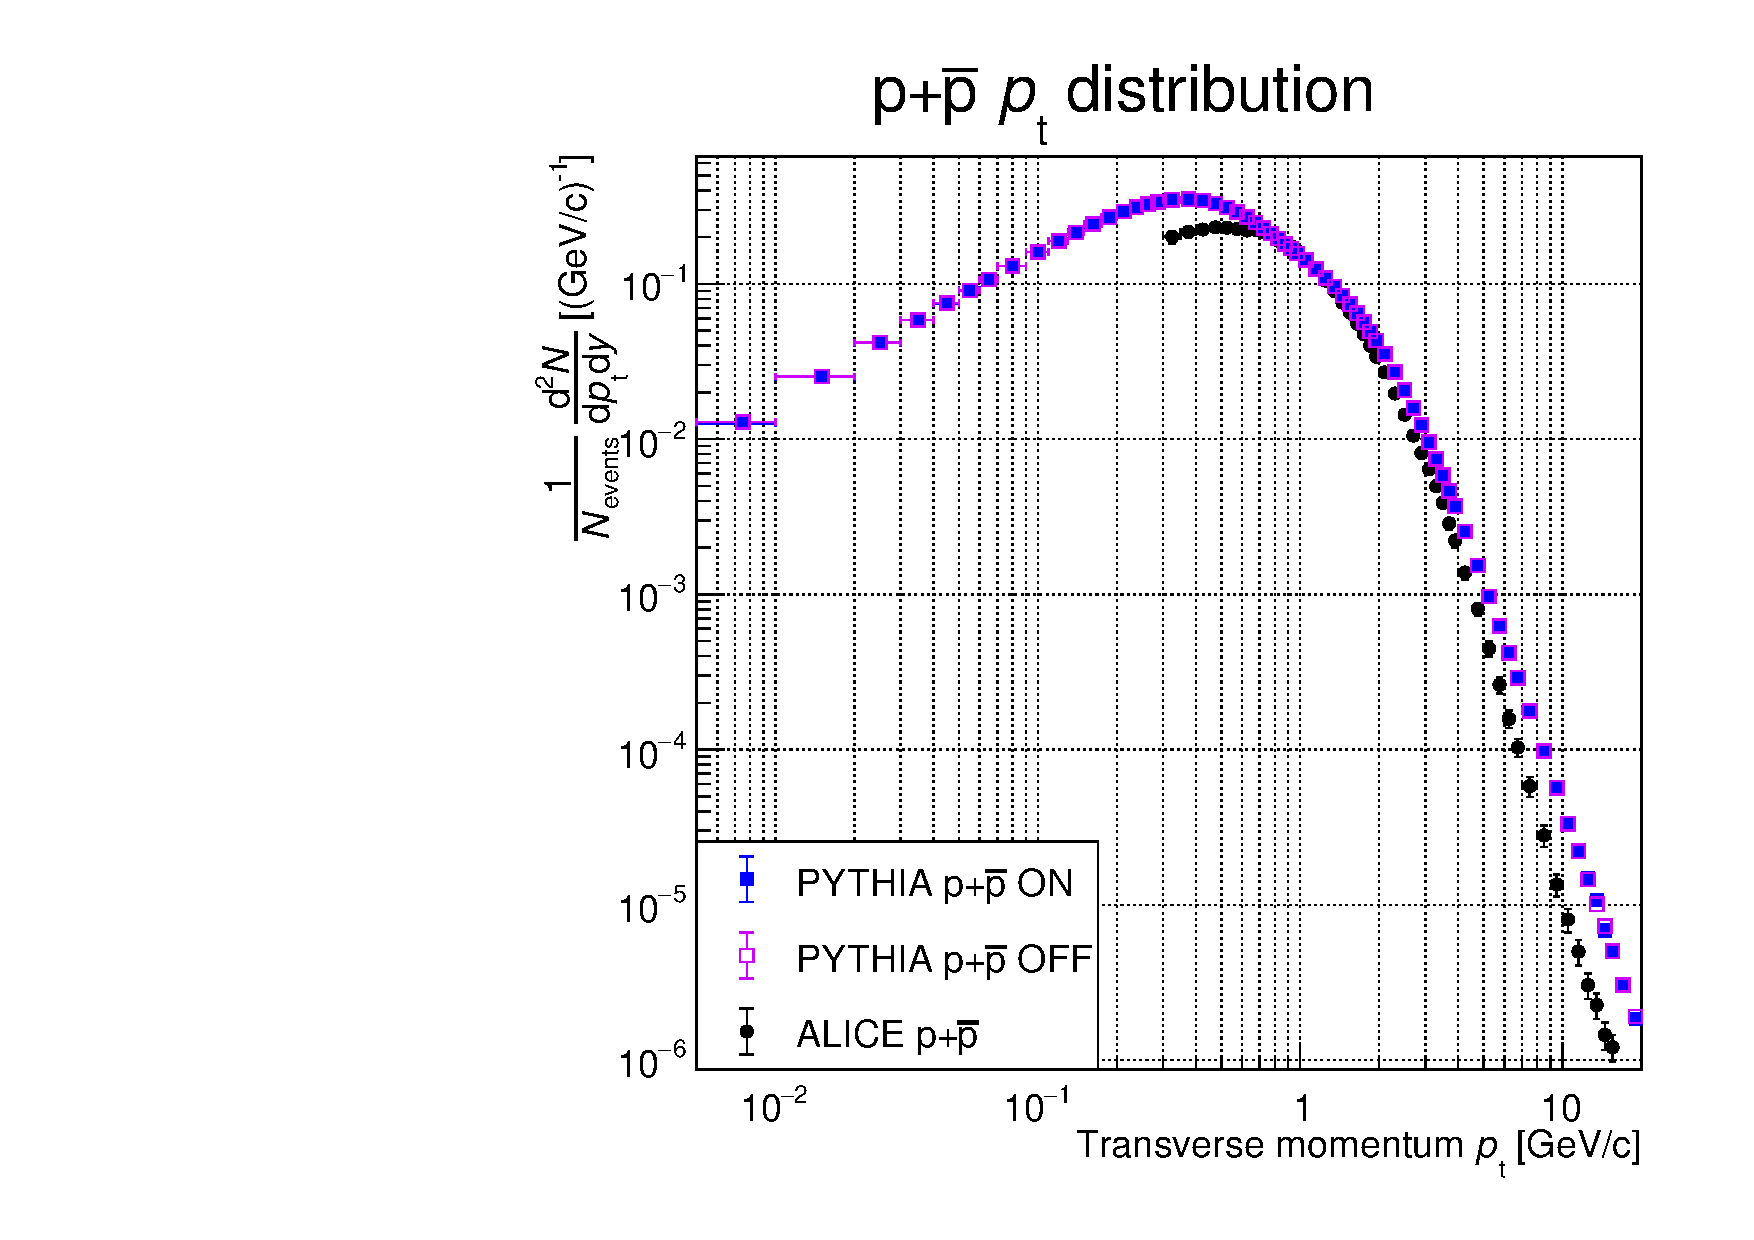
\includegraphics[width=\textwidth]{image/3-risultati/analyse/G/pp.pdf}
        \caption{}
        \label{fig:D_pp}
    \end{subfigure}
    %\hspace{1cm}
    \begin{subfigure}{.49\textwidth}
        \centering
        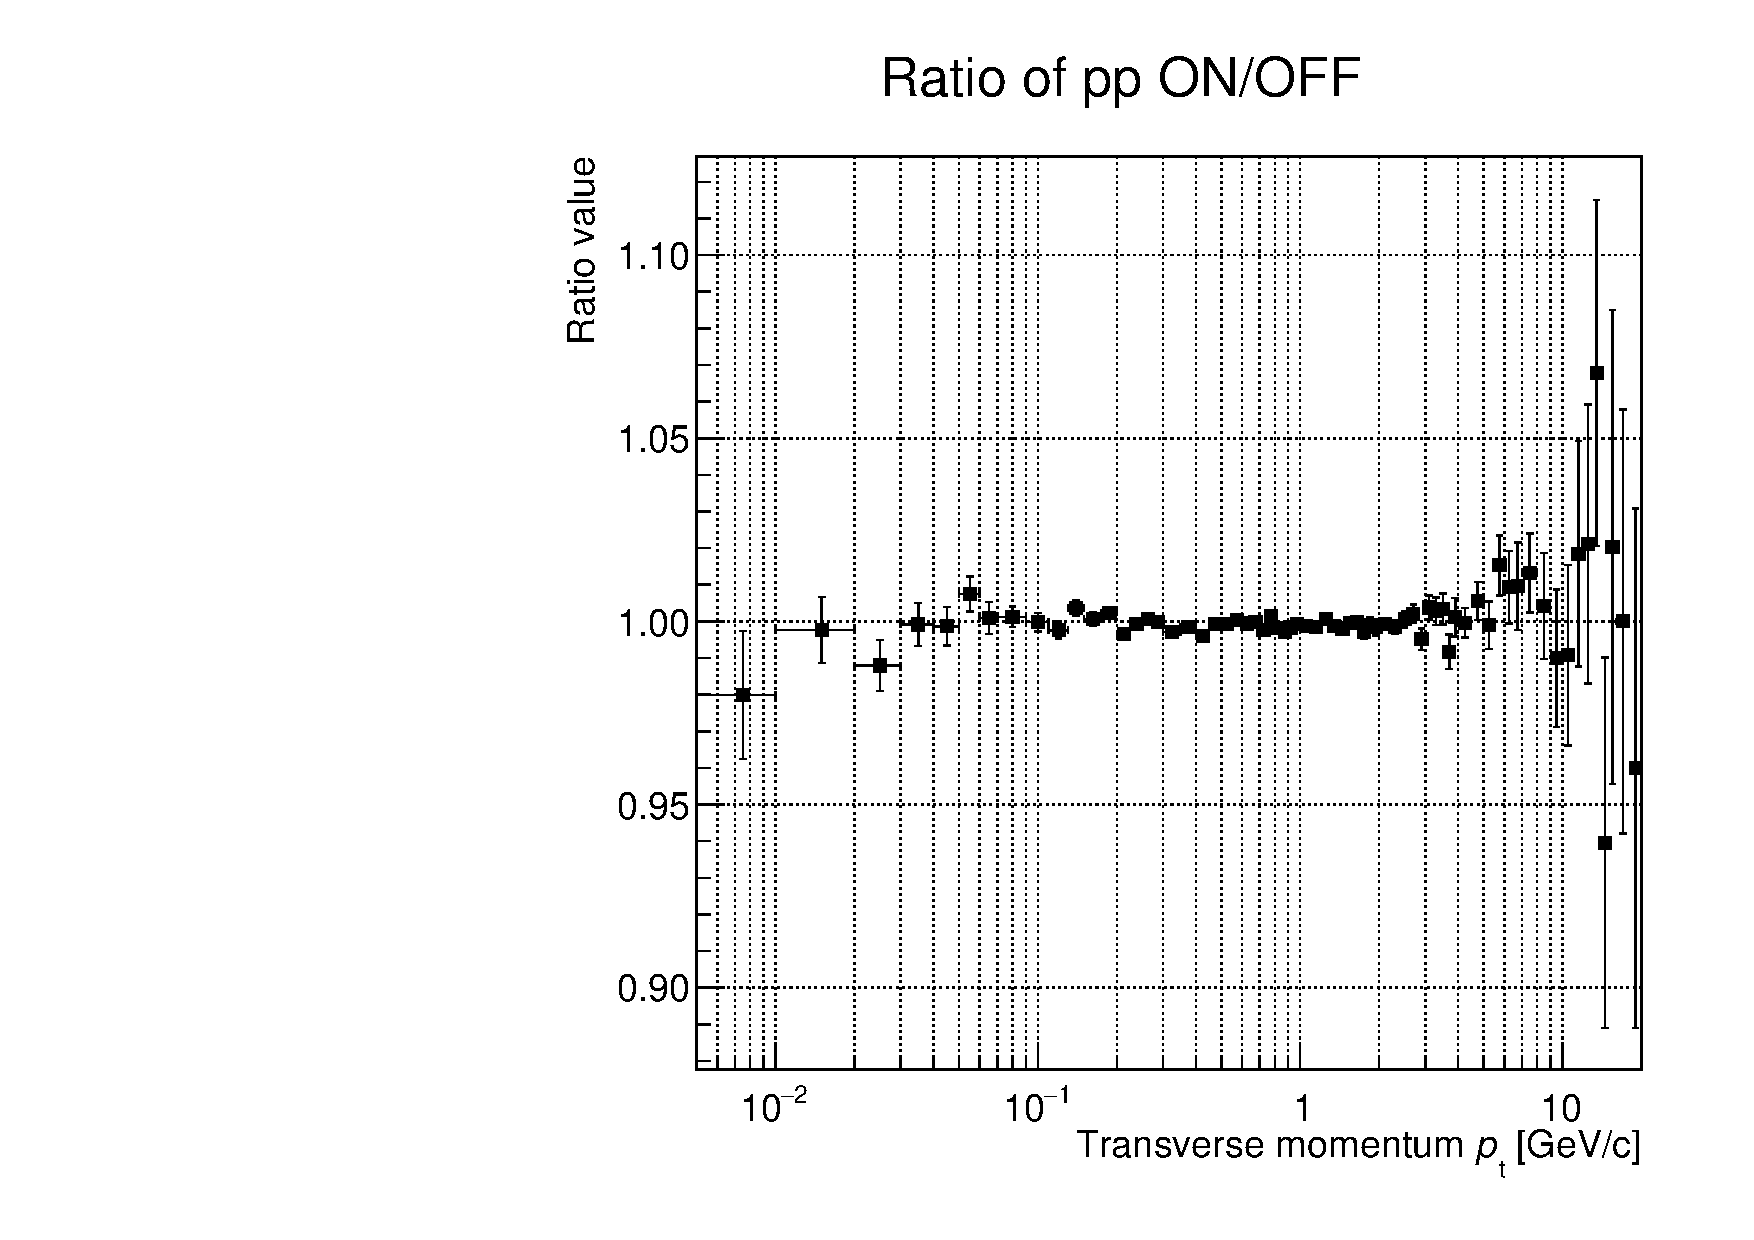
\includegraphics[width=\textwidth]{image/3-risultati/analyse/G/ratio_pp_ON_OFF.pdf}
        \caption{}
        \label{fig:D_ratio_pp_ON_OFF}
    \end{subfigure}
    \captionwithsource{\emph{\rmfamily (a)} Distribuzione dell'impulso trasverso di $p+\bar p$ con produzione deuteronica attivata e disattivata ("ON" e "OFF") in confronto con i dati sperimentali di ALICE ("ALICE"), usando il modello ottimizzato. \emph{\rmfamily (b)} Frazione della distribuzione dell'impulso trasverso di $p+\bar p$ con produzione deuteronica attivata e con produzione non attivata, usando il modello ottimizzato.}{\cite{ALICE:2020jsh}}
    \label{fig:D_pp_prod}
\end{figure}
Neanche il rapporto tra il caso in cui la produzione deuteronica sia attivata e quella disattivata presenta particolari differenze, come si può notare in \autoref{fig:D_ratio_pp_ON_OFF}, con un valore della media pesata di $0.99889 \pm 0.00024$, vicino al valore di 0.999.

Per quanto riguarda gli spettri dei (anti)deuteroni (in \autoref{fig:D_(anti)deuteron}) essi mostrano un accordo migliore con i dati rispetto al modello predefinito, come si può osservare in \autoref{fig:A_(anti)deuteron}.
Ciò è supportato andando a effettuare una divisione tra i dati dei (anti)deuteroni di \pythia{} e di ALICE ottenendo così il grafico riportato in \autoref{fig:D_division}.
Come già anticipato, il valore della media pesata del rapporto è di $1.0467 \pm 0.015$ per i deuteroni e $ 0.968 \pm 0.021$ per gli antideuteroni, più vicini al valore unitario rispetto a quello del modello predefinito.

Anche qui si esegue una verifica della correttezza delle simulazioni andando a vedere il bilancio deuteroni-antideuteroni.
Effettuando una divisione tra gli istogrammi dei deuteroni e degli antideuteroni (\autoref{fig:D_ratio_DD}), si ottiene un valore della media pesata di $1.017 \pm 0.008$, compatibile entro 3 sigma con il valore unitario.\\

Per ultimo si esegue un confronto tra i due modelli.
Si ottiene il grafico visibile in \autoref{fig:def_opt}.
È importante notare come le distribuzioni di produzione di (anti)deuterone in funzione dell'impulso trasverso ottenute con i due modelli abbiano in realtà lo stesso identico andamento ma valori assoluti diversi; ciò è dovuto al fatto che le variazioni del parametro \ttbox{norm} agiscono sul numero complessivo di (anti)deuteroni prodotti in tutti i canali di produzione.
Gli spettri prodotti hanno quindi la medesima forma ma un differente fattore di scala.
\begin{figure}[htp]
    \centering
    \begin{subfigure}{.49\textwidth}
    \centering
        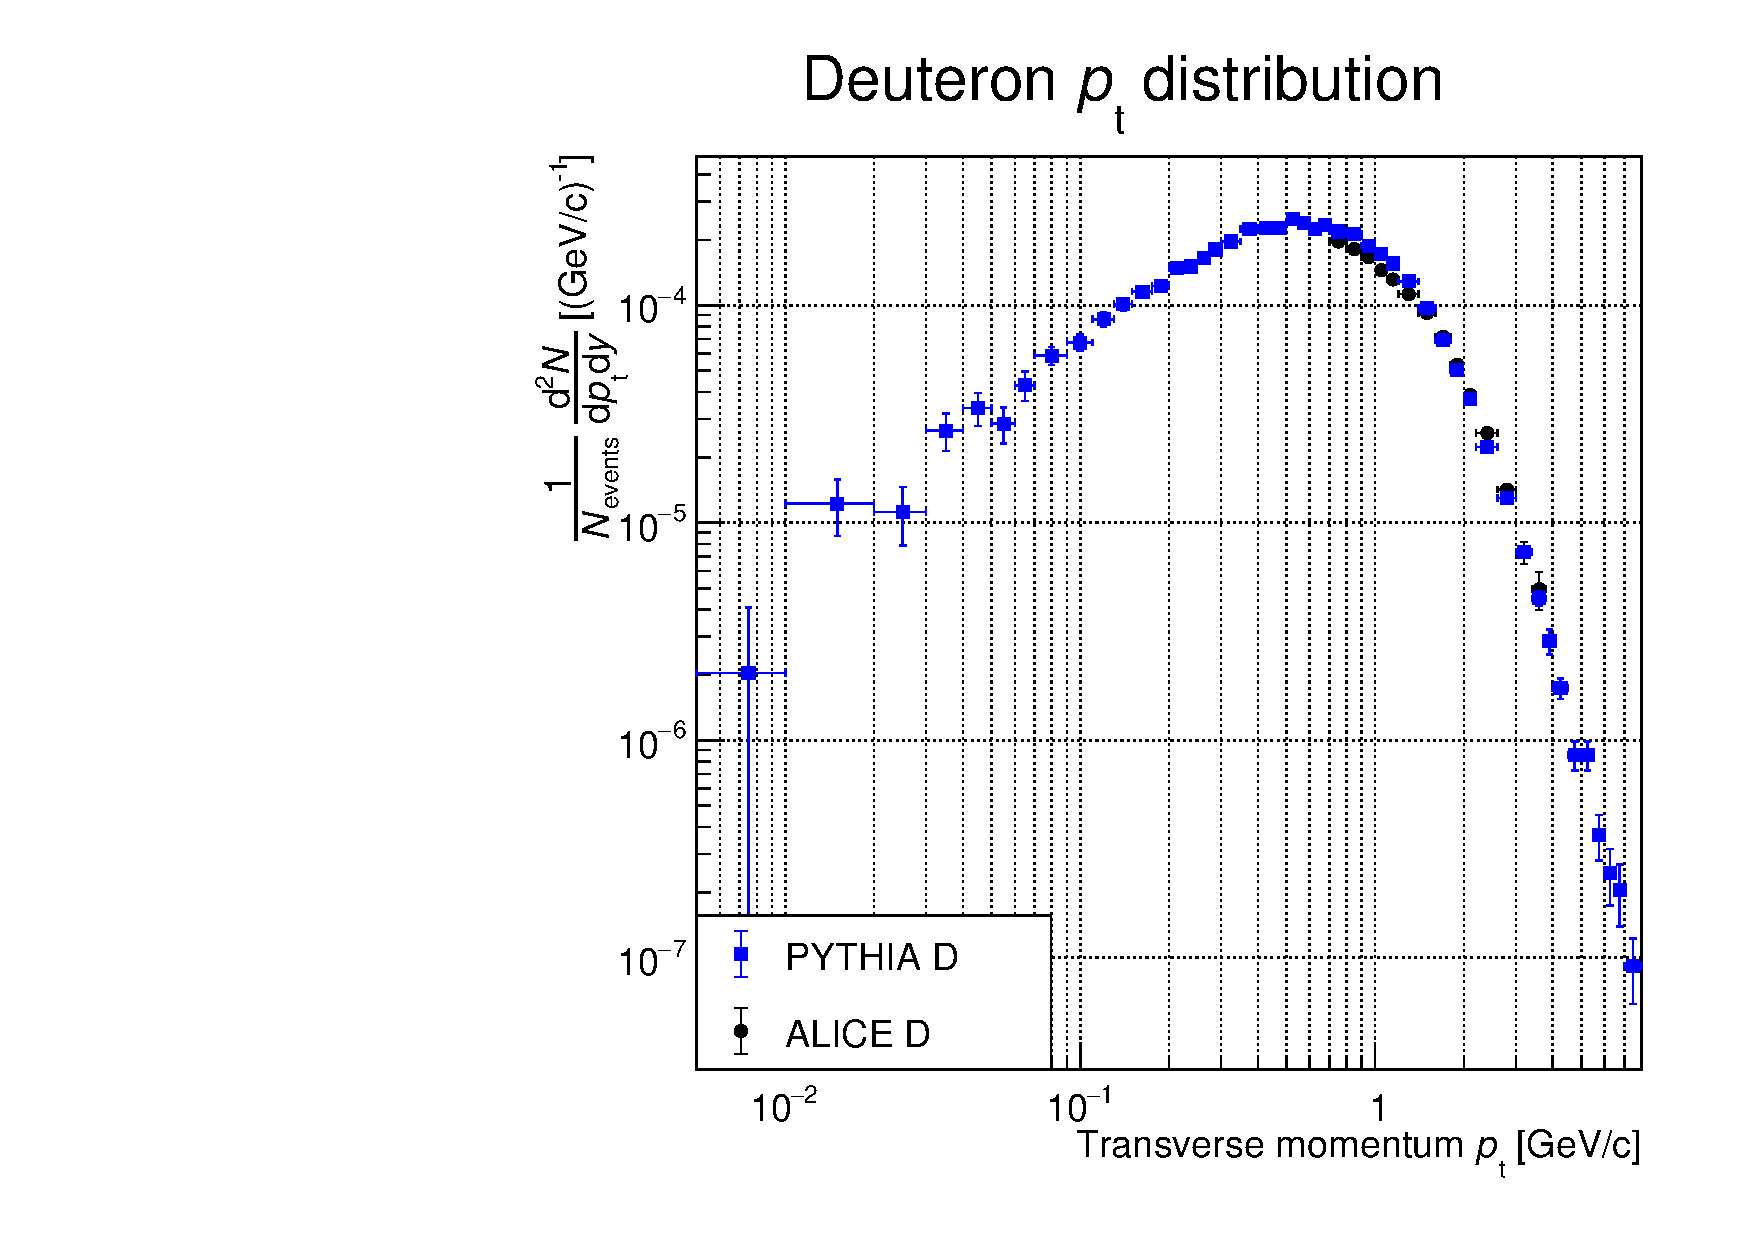
\includegraphics[width=\textwidth]{image/3-risultati/analyse/G/deuteron.pdf}
        \caption{}
        \label{fig:D_deuteron}
    \end{subfigure}
    %\hspace{1cm}
    \begin{subfigure}{.49\textwidth}
        \centering
        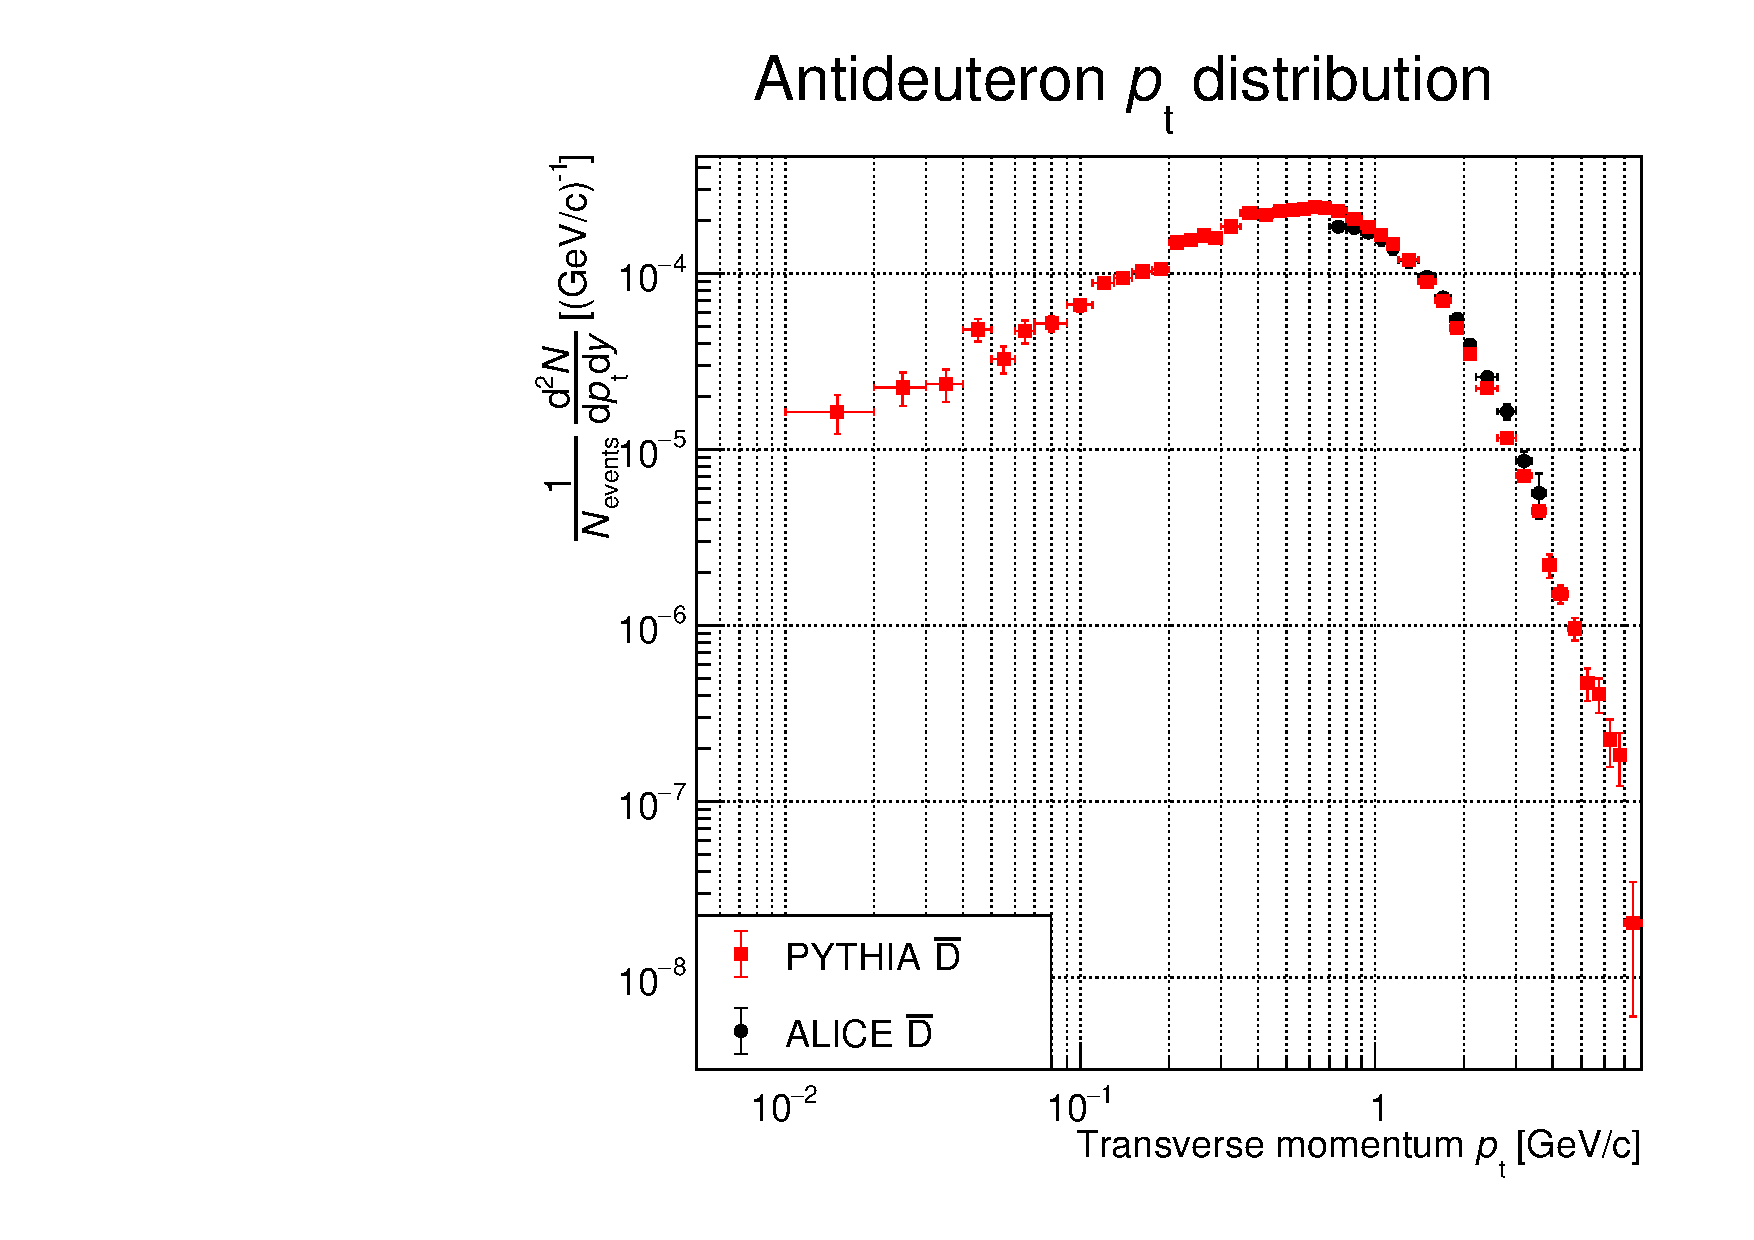
\includegraphics[width=\textwidth]{image/3-risultati/analyse/G/antideuteron.pdf}
        \caption{}
        \label{fig:D_antideuteron}
    \end{subfigure}
    \captionwithsource{Distribuzione dell'impulso trasverso di \emph{\rmfamily (a)} $D$ e \emph{\rmfamily (b)} di $\bar D$ in confronto con i dati di ALICE, utilizzando il modello ottimizzato.}{\cite{ALICE:2020foi}}
    \label{fig:D_(anti)deuteron}
\end{figure}
\begin{figure}[htp]
    \centering
    \begin{subfigure}{.49\textwidth}
    \centering
        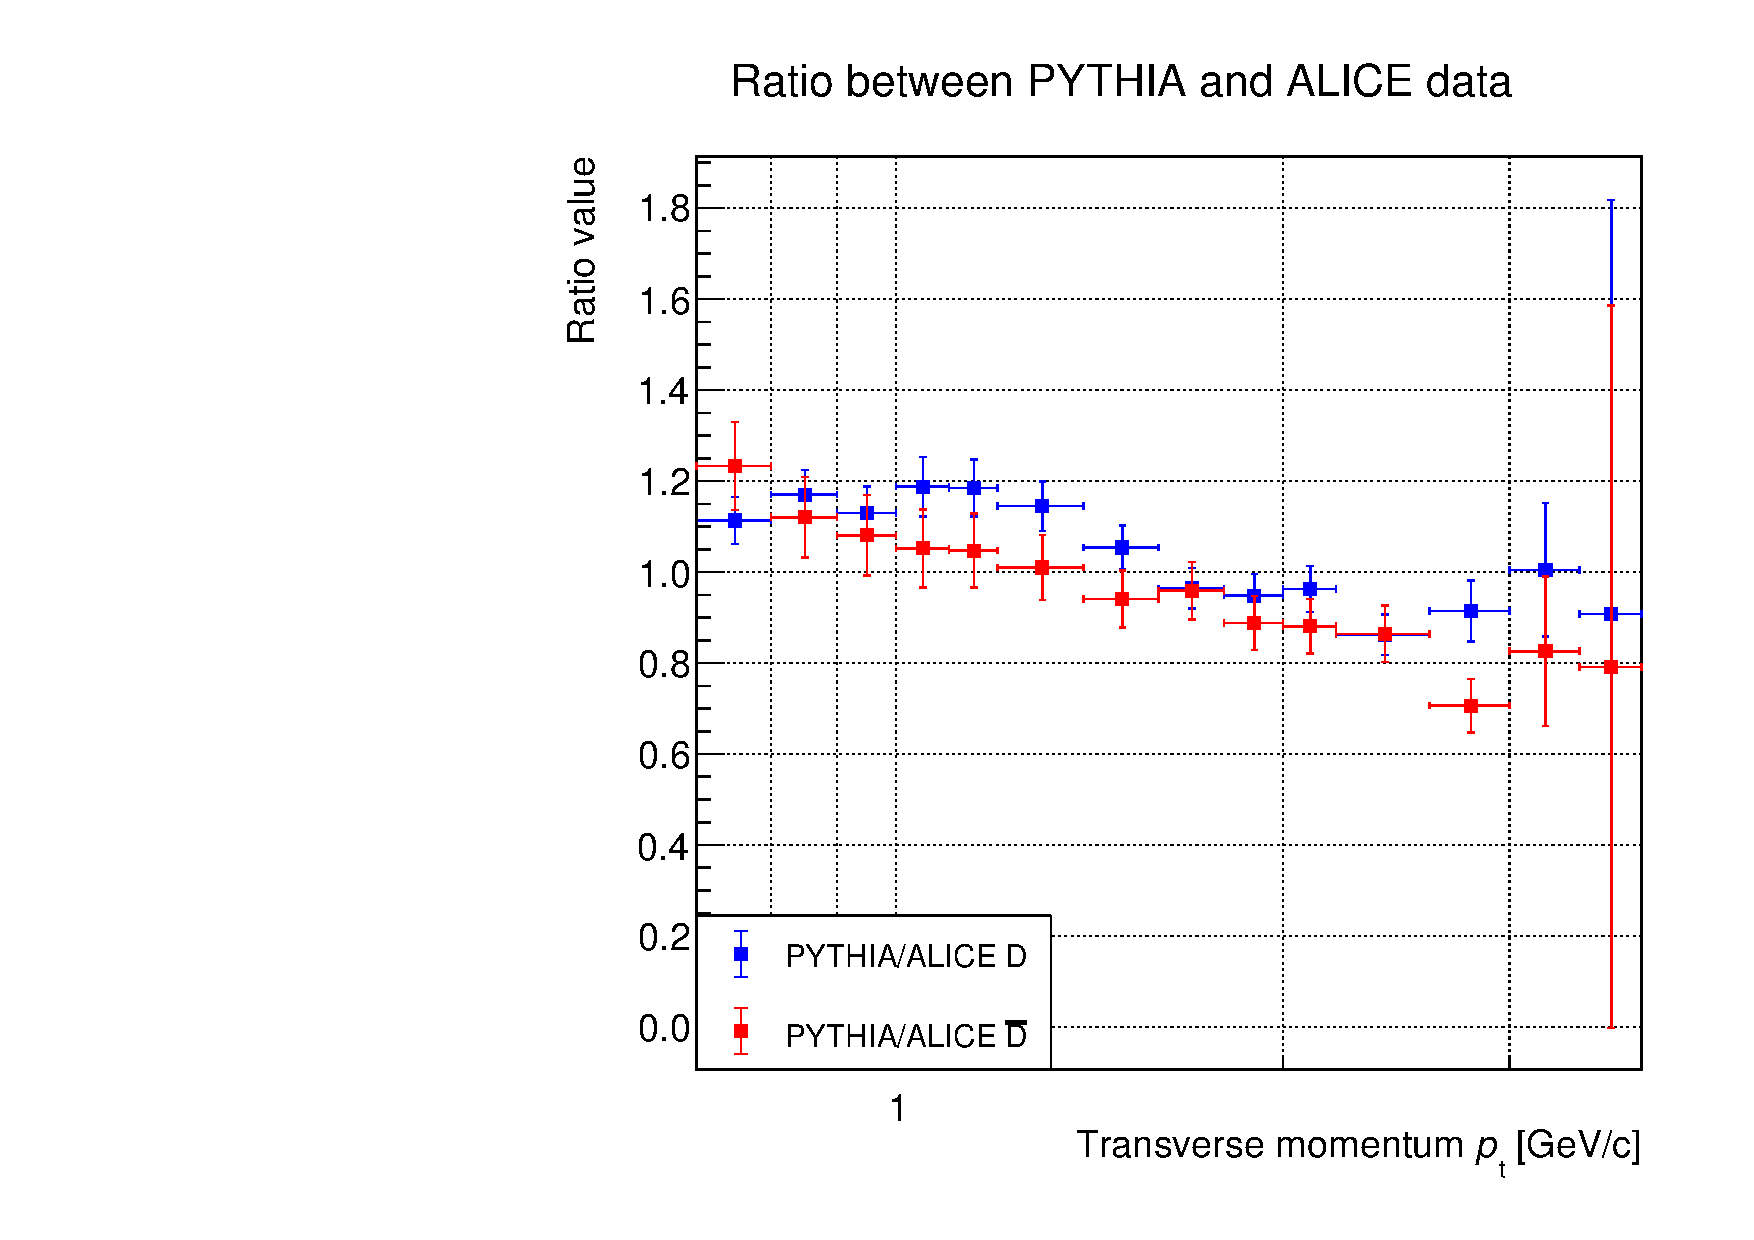
\includegraphics[width=\textwidth]{image/3-risultati/analyse/G/division.pdf}
        \caption{}
        \label{fig:D_division}
    \end{subfigure}
    %\hspace{1cm}
    \begin{subfigure}{.49\textwidth}
        \centering
        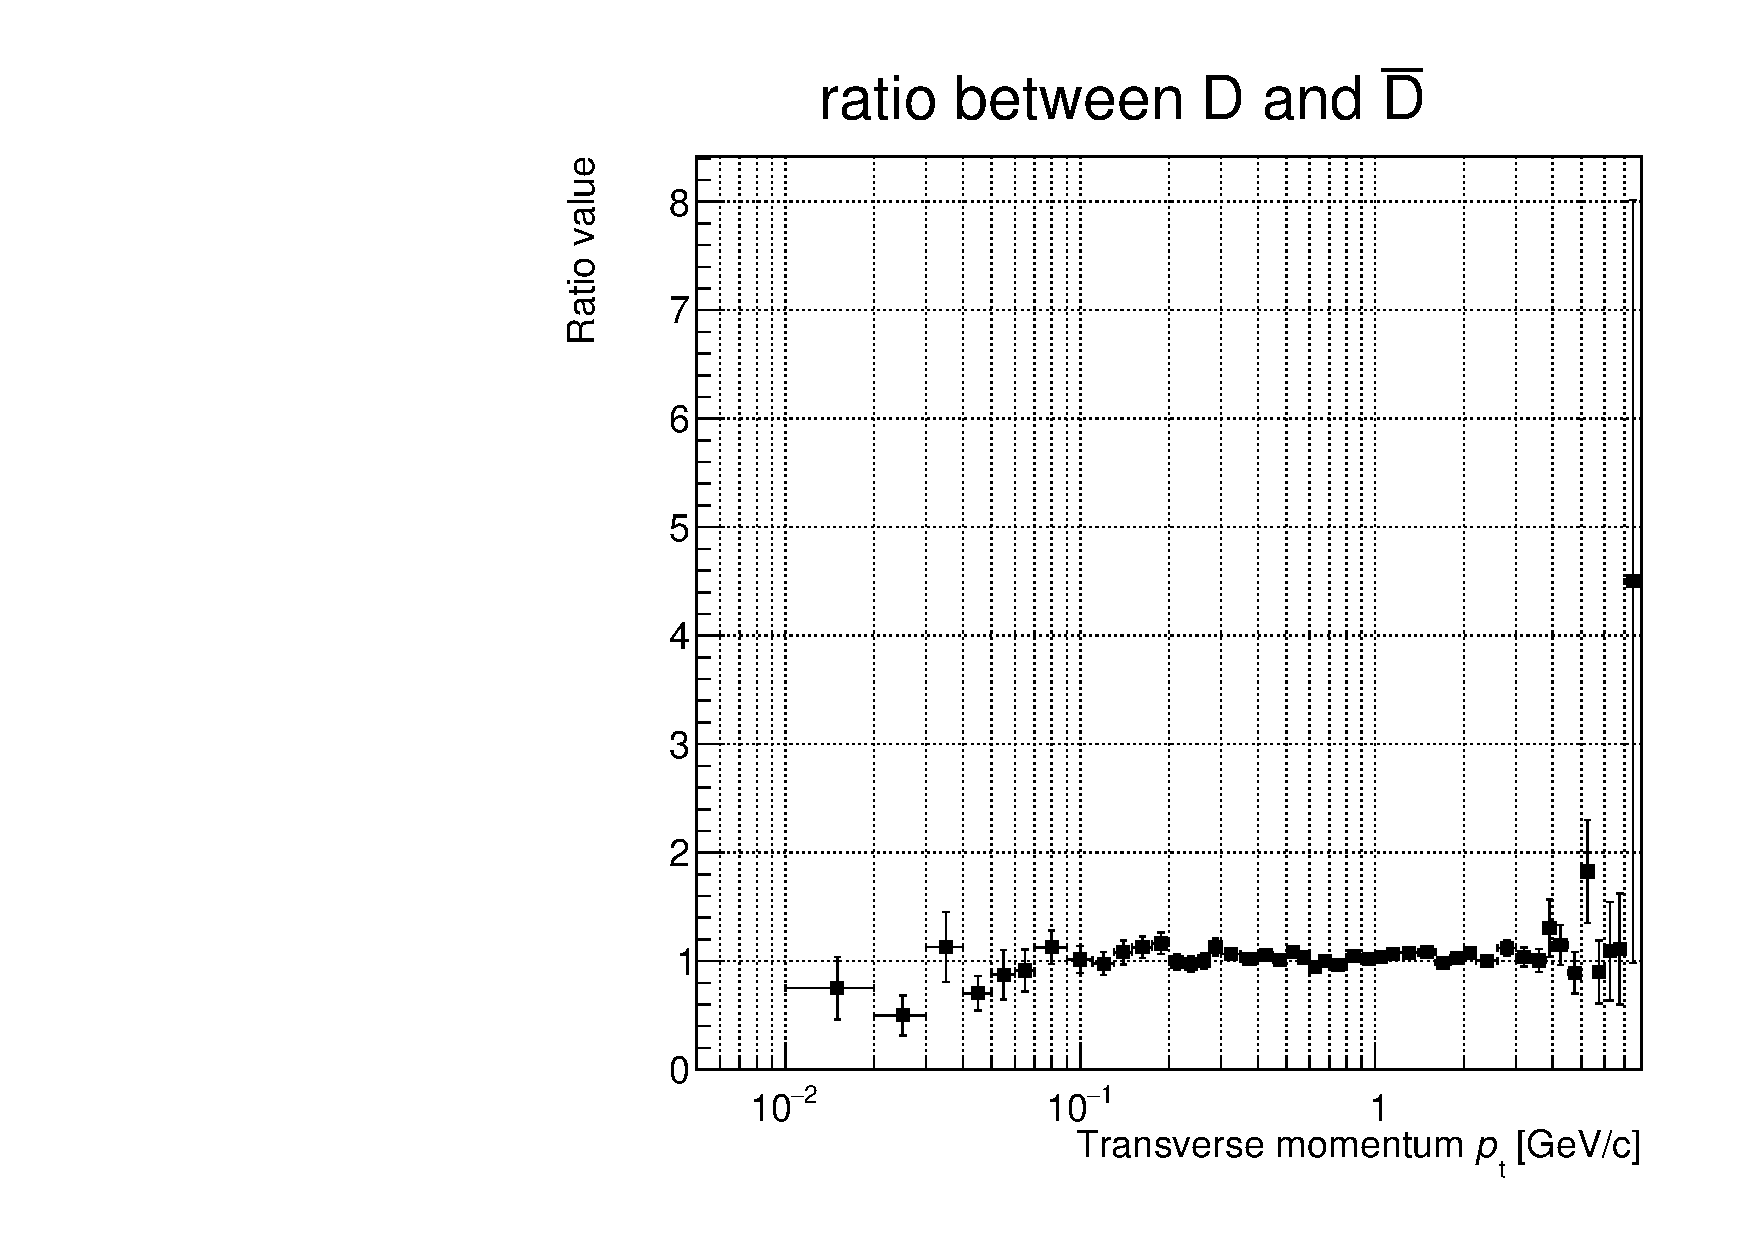
\includegraphics[width=\textwidth]{image/3-risultati/analyse/G/ratio_DD.pdf}
        \caption{}
        \label{fig:D_ratio_DD}
    \end{subfigure}
    \caption{\emph{\rmfamily (a)} Divisione tra la distribuzioni dell'impulso trasverso di $D$ e $\bar D$ con i dati di ALICE, utilizzando il modello ottimizzato. \emph{\rmfamily (b)} Frazione delle distribuzione dell'impulso trasverso di $D$ con quello di $\bar D$, utilizzando il modello ottimizzato.}
    \label{fig:D_ratio_DD_}
\end{figure}
\begin{figure}[h]
    \centering
    \begin{subfigure}{.49\textwidth}
    \centering
        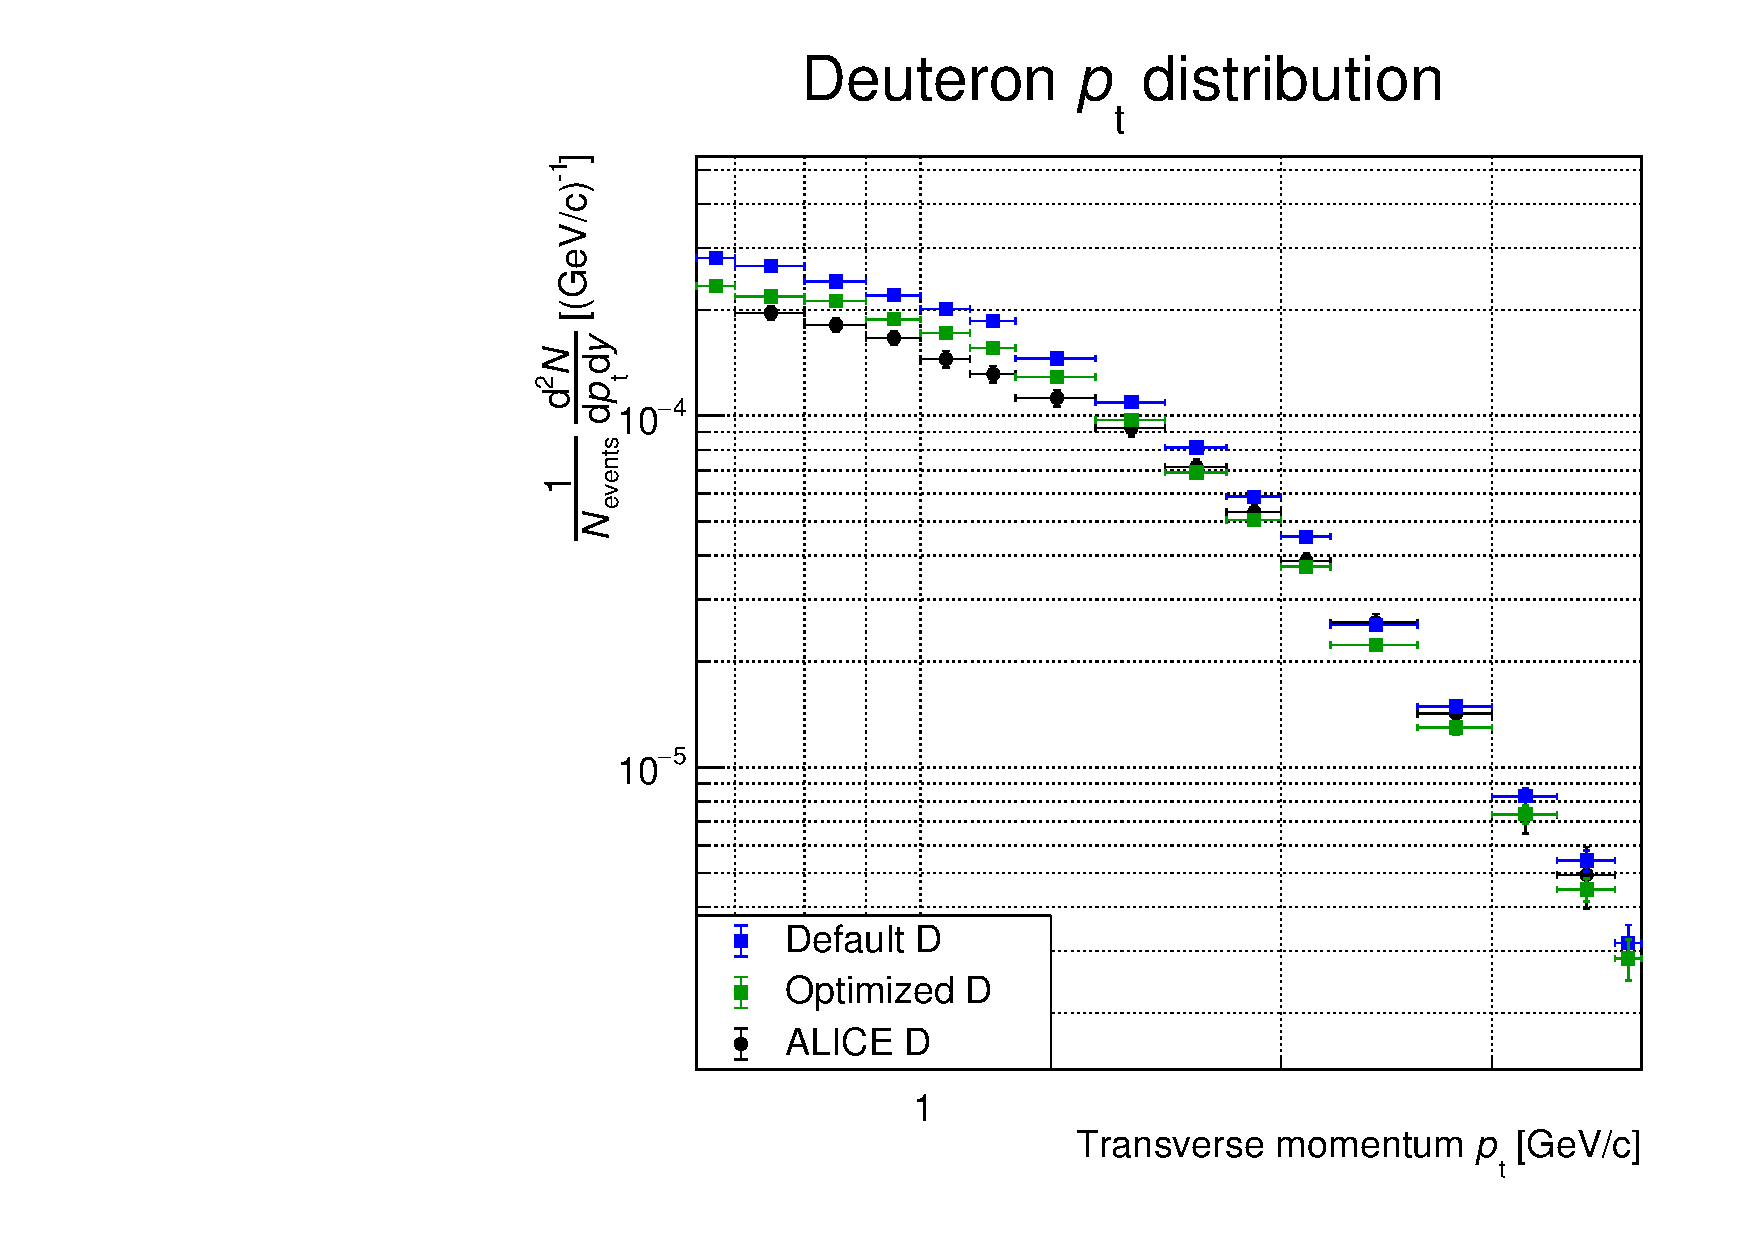
\includegraphics[width=\textwidth]{image/3-risultati/analyse/G/def_opt_deuteron.pdf}
        \caption{}
        \label{fig:def_opt_deuteron}
    \end{subfigure}
    %\hspace{1cm}
    \begin{subfigure}{.49\textwidth}
        \centering
        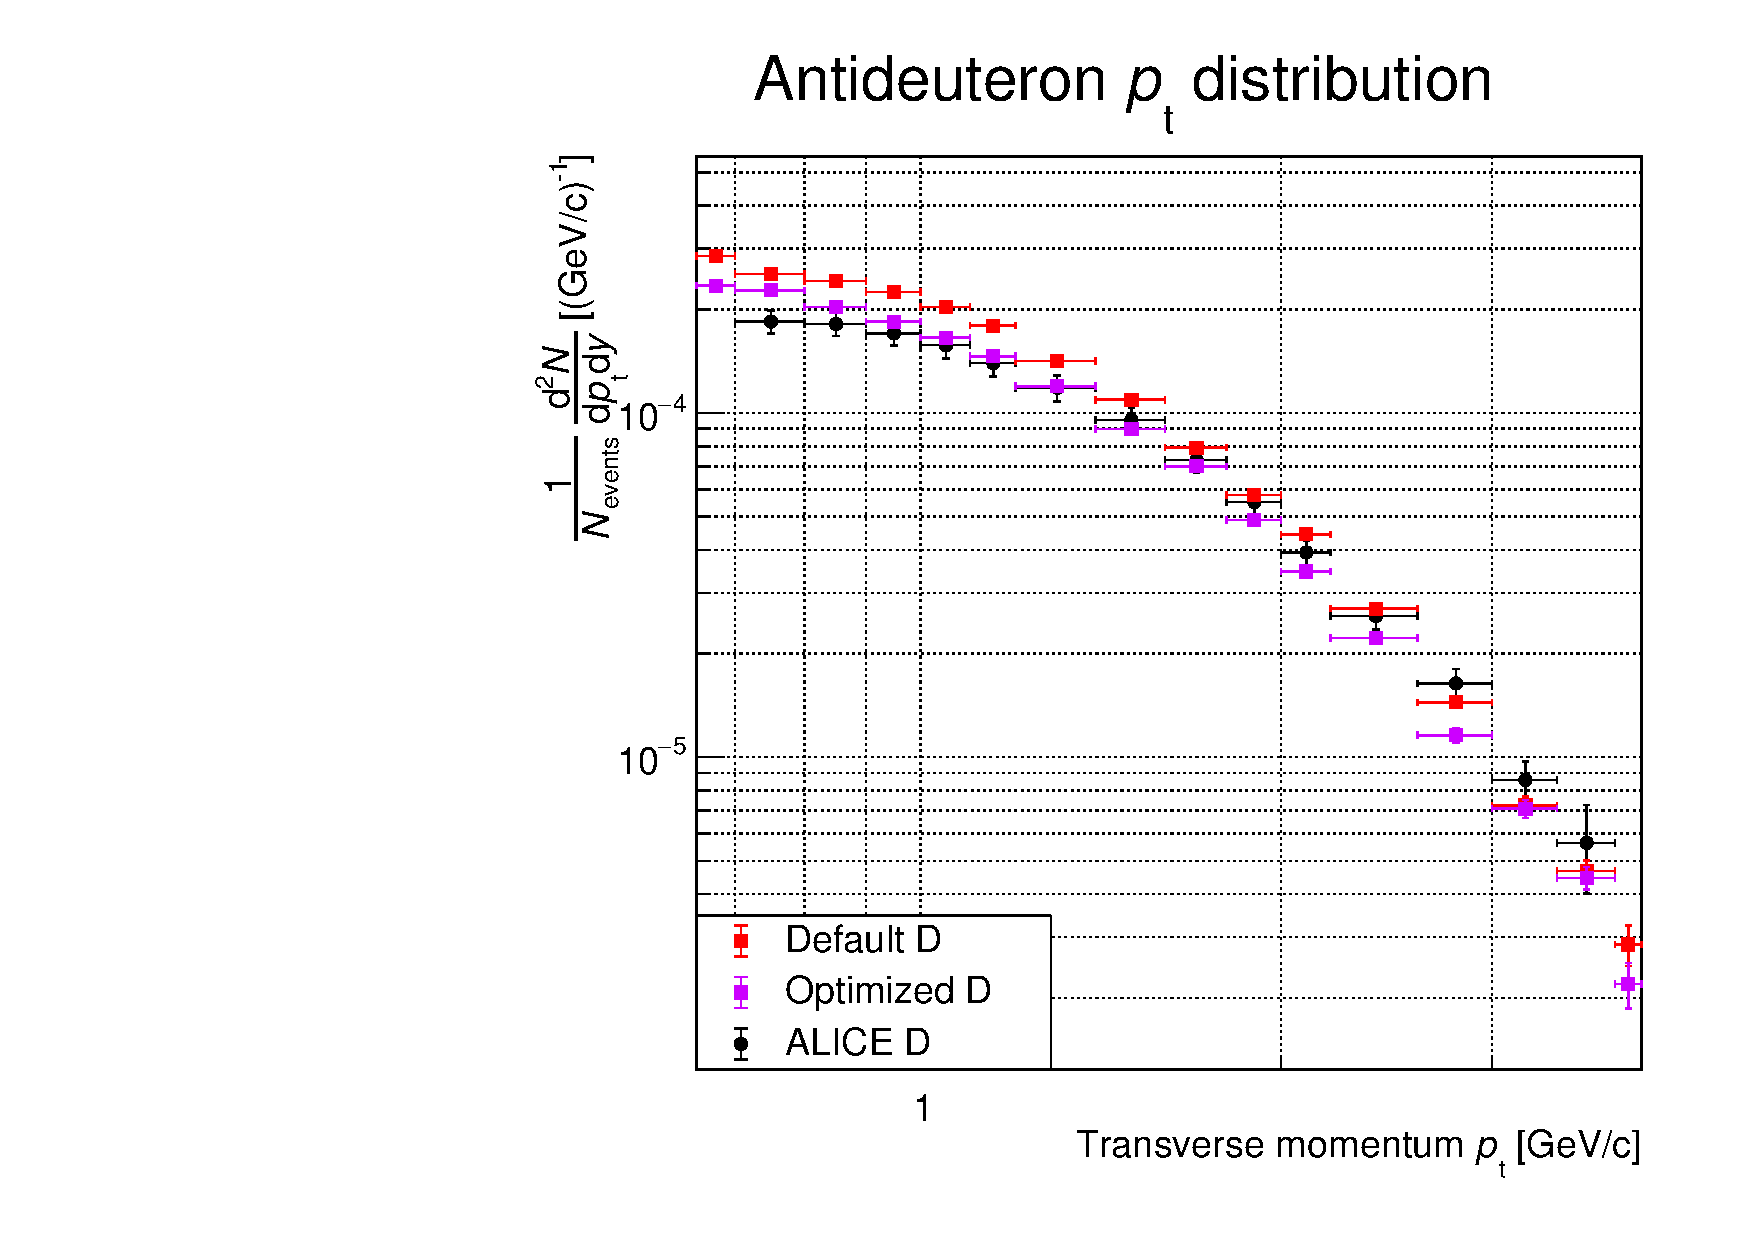
\includegraphics[width=\textwidth]{image/3-risultati/analyse/G/def_opt_antideuteron.pdf}
        \caption{}
        \label{fig:def_opt_antideuteron}
    \end{subfigure}
    \captionwithsource{Distribuzioni dell'impulso trasverso dei deuteroni e dei antideuteroni del modello predefinito ("Default"), ottimizzato ("Optimized") e dei dati di ALICE.}{\cite{ALICE:2020foi}} 
    \label{fig:def_opt}
\end{figure}

\chapter*{Conclusioni}
\markboth{Conclusioni}{Conclusioni}
\addcontentsline{toc}{chapter}{Conclusione}
In questo lavoro di tesi si è descritto lo stato dell'arte degli studi sul Quark Gluon Plasma (QGP), dando una visione sperimentale con una panoramica dell'esperimento ALICE, dei suoi rilevatori e dei suoi principali obiettivi nel campo della fisica.
Grazie alle eccellenti capacità di tracciamento e di identificazione di particelle, ALICE ha permesso di studiare nel dettaglio le proprietà e l'evoluzione dello stato di QGP ricreato nelle collisioni di ioni pesanti ultrarelativistici a LHC, permettendo di verificare i diversi modelli teorici sviluppati nel corso degli ultimi anni.
Attenzione particolare è stata data alla descrizione delle tecniche di misura di nuclei e antinuclei leggeri che sono prodotti all'LHC in uguale quantità.

Successivamente sono stati introdotti e descritti i due modelli attualmente più utilizzati per descrivere la produzione di (anti)nuclei leggeri: il modello di coalescenza di (anti)nucleoni nello stadio finale della collisione e il modello di adronizzazione statistica.
Per entrambi i modelli sono stati evidenziati i punti di forza e i limiti tramite un confronto con i dati raccolti da ALICE.
Successivamente si è introdotto il generatore Monte Carlo \pythiaa{}, software ampiamente utilizzato per la simulazione di eventi della fisica di particelle.
Di \pythiaa{} si è evidenziato il suo modello teorico di produzione deuteronica, ossia il modello di sezioni d'urto efficaci.

Il lavoro principale di questa tesi è stato quello di utilizzare il software \pythiaa{} per simulare eventi di collisione pp a $\sqrt{s} = 13$ TeV, confrontando le simulazioni con i dati sperimentali misurati da ALICE e analizzando nel dettaglio i canali di produzione dei deuteroni, determinandone i principali contributi.
Inoltre si è andati a confrontare il modello di sezioni d'urto efficaci con il modello di coalescenza, sempre implementato in \pythiaa{}, mostrando quali siano le differenze tra i due modelli.
Infine, è stato effettuato uno studio di ottimizzazione del parametro \ttbox{DeuteronProduction:norm} del modello di sezioni d'urto efficaci.
Il parametro ottimizzato assume il valore di circa 140.46, corrispondente a un valore di $1/\sigma_0$ di circa 2.24 \si{barn^{-1}}.
Sebbene le simulazioni condotte con \pythiaa{} e i parametri ottimizzati in questa tesi non siano ancora in grado di riprodurre completamente gli spettri di (anti)deuterone misurati da ALICE, i risultati mostrano un accordo sensibilmente migliore rispetto alle configurazioni di default di \pythiaa{}:
infatti nel modello predefinito vi è una sovrapproduzione sia dei deuteroni sia dei antideuteroni (rispettivamente circa del 20\% e del 13\%), mentre utilizzando il modello ottimizzato si ha una sovrapproduzione di deuteroni del circa 3.6\% e una sottoproduzione di antideuteroni del circa 6\%.

In conclusione il lavoro presentato in questa tesi ha cercato di fornire una motivazione per lo studio della produzione di (anti)deuteroni, ha descritto quali sono i modelli teorici più utilizzati per descrivere i meccanismi di nucleosintesi, ha sfruttato il software \pythiaa{} per le simulazioni Monte Carlo e infine ha permesso di trovare una configurazione di \pythiaa{} in grado riprodurre in maniera più fedele i dati sperimentali raccolti da ALICE.

% bibliografia (il path è dentro leo_preamble.sty)
\pagestyle{bib}
\printbibliography[nottype=online]
\addcontentsline{toc}{chapter}{Bibliografia}

\end{document}